\documentclass[]{article}

\def\nno{\nonumber}
\def\bfE{\mbox{\boldmath$E$}}
\def\bfG{\mbox{\boldmath$G$}}
\def \p{\partial}
\usepackage{epsfig, color}
\usepackage{color,graphicx}
\usepackage{amsfonts}
\usepackage{color}
\usepackage{amsmath}
\usepackage{amssymb}
\usepackage{amsthm}
\usepackage[backend=bibtex,citestyle=authoryear, maxcitenames=1]{biblatex}

\addbibresource{bib}
\DeclareCiteCommand{\cite}
{\color{blue}\usebibmacro{prenote}}%
{\usebibmacro{citeindex}%
	\usebibmacro{cite}}
{\multicitedelim}
{\usebibmacro{postnote}}


\usepackage{fancybox}
\usepackage{ulem}
\usepackage{subfigure}
\usepackage{multirow}
\usepackage{bbm}
\usepackage{enumerate}
\usepackage{rotating}
\usepackage{float}
\usepackage{epstopdf}
\usepackage{tcolorbox}
\usepackage{mdframed}
\usepackage{framed}
\usepackage{graphbox}
\usepackage{makecell}
\usepackage{diagbox}
\usepackage{booktabs}
\usepackage{threeparttable}
\usepackage{appendix}
\usepackage{hyperref}
\usepackage{longtable}
%\usepackage{refcheck}

\allowdisplaybreaks[4]

\newtheorem{definition}{\hspace{6mm}Definition}[section]
\newtheorem{theorem}{\hspace{6mm}Theorem}[section]
\newtheorem{lemma}{\hspace{6mm}Lemma}[section]
\newtheorem{remark}{\hspace{6mm}Remark}[section]
\newtheorem{example}{\textsc{Example}}[section]
\newtheorem{proposition}{\hspace{6mm}Proposition}[section]
\newtheorem{algorithm}{Algorithm}
\renewcommand{\(}{\left(}
\renewcommand{\)}{\right)}
\newcommand{\bm}[1]{\mbox{\boldmath{$#1$}}}
\def\cred{\color{red}}
\def\cpurp{\color{purple}}
\def\cblue{\color{blue}}
\def\cgreen{\color{green}}

%opening
\title{\cred{Integrating Path Signatures and Transformers: A Novel Approach for Calibrating Rough Volatility Models\footnote{\cred{Chiheb's edits are in red}}}}
\author{}
\date{}

\begin{document}
	\maketitle
	\begin{abstract}
		In this paper, we present a new model, named the SigFormer\footnote{\cred{I think we are not exactly using same architecture as the authors of Sigformer, so maybe better to avoid using same acronym}}\footnote{"\textcolor{blue}{ConvSigMA}" is one possible alternative name for our model, since it combines elements from \textcolor{blue}{Conv}olutional layers, path \textcolor{blue}{Sig}nature transform and \textcolor{blue}{M}ulti-head \textcolor{blue}{A}ttention mechanisms.} model, based on both the self-attention mechanism and the signature transform to calibrate volatility processes simulated by various rough volatility models. We also provide numerical examples to demonstrate its advantages in the calibration of both single and multiple parameters. Code is available at \href{github.com/changanluoxue/signature-transform}{github.com/changanluoxue/signature-transform}.
		
		\cred{\footnote{\cred{Chiheb's abstract version}}The calibration of stochastic differential equations is crucial for several applications, especially in quantitative finance.  This work presents an innovative machine learning method for calibrating rough volatility models, specifically rough Bergomi and rough Heston models. We leverage path signatures for feature mapping and transformers for their attention mechanism to calibrate both the Hurst parameter and other model parameters efficiently.  Our empirical study demonstrates the superiority  of our approach  in terms of accuracy for the  calibration  for  both single and multiple parameters over existing methods, including convolutional neural networks  \parencite{stone_2020} and deep signature techniques \parencite{Lyons_2019_DeepSignature}.
			The code is available at \href{https://github.com/changanluoxue/signature-transform.git}{github.com/changanluoxue/signature-transform}.\footnote{\cred{For the code link, we may create later another seperate repository (from the current internal one) having only the code.}}}
	\end{abstract}
	
	\section{Introduction}\label{sec-introduction}
	The effective calibration for rough volatility models represents a crucial challenge in the field of mathematical finance. Over the years, various neural networks based calibration approaches have been developed. These approaches can be categorized by the different types of neural networks they are based. Since the fully connected feed forward neural network is the basic neural network model, there are many references use it directly for calibration (see e.g., \cite{horvath2021deep}, \cite{rosenbaum2021deep}). The fully connected feed forward neural network can also be integrated into the stochastic Volterra integral equations to calibrate more precisely (see e.g., \cite{wang2021NSDE}, \cite{ma2023rough}). Furthermore, \cite{stone_2020} verified that the convolutional neural network can also be used for calibrating rough volatility models. \cite{Lyons_2019_DeepSignature} introduced the signature based neural network to calibrate fractional Brownian motions. 
	
	Recently, large-scale natural language processing models (LLMs) have been developed rapidly thanks to the transformer model proposed by \cite{vaswani_2017}. It is nature to think that whether the transformer can improve the performance of existing neural networks based calibration approaches since the volatility data is also sequential. The aim of this paper is to explore a appropriate combination method for transformer and existing neural networks based calibration approaches to calibrate rough volatility models.
	
	In this paper, we use the self-attention mechanism with signature transform as a layer in a neural network to investigate whether this architecture can help to calibrate parameters from a set of rough paths and we follow \cite{tong_2023} to call it SigFormer model. The structure of the paper is the following. In Section~\ref{sec-background}, we give a brief introduction to the rough volatility models, path signature theory and attention mechanism that we will use in this paper. The specific architecture of our SigFormer model is clarified in Section~\ref{sec-methodology}. In Section~\ref{sec-experiments}, we begin with a simple SigFormer model, only consisting of the signature transform layer and single-head attention layer, to present the evolution leading to our SigFormer model. Finally, we discuss our conclusions in Section~\ref{sec-conclusion}.
	\section{Background}\label{sec-background}
	\textcolor{blue}{In this section, we first formalize the calibration problem and then give a brief but necessary introduction to the rough volatility models, path signature theory and attention mechanism.}

	\textcolor{blue}{\subsection{Problems formalization}\label{subsec-formalization}
	In our context, the rough volatility model calibration is meant to find the model parameters such that the model is as close as possible to the observed volatility path. To formalize this, let us first define a stream $X^n\in\mathbb{R}^{n\times d}$ with $n,\,d\in\mathbb{N}^+$ as the observed path and $\theta_V\in\mathbb{R}^{l_V}$ with $l_V\in\mathbb{N}^+$ represents parameters corresponding to the observed path in the rough volatility model i.e. the target of this calibration problem. Then the rough volatility model calibration can be formalized as 
	\begin{eqnarray}
		\widehat{\theta}_M&=&\arg\min\limits_{\theta_M}\delta\left(\mathcal{M}\(X^n;\,\theta_{M}\),\,\theta_V\right),\\
		\widehat{\theta}_V&=&\mathcal{M}\(X^n;\,\widehat{\theta}_{M}\),
	\end{eqnarray}
	where $\mathcal{M}(\theta_M):\mathbb{R}^{n\times d} \mapsto \mathbb{R}^{l_V}$ is an abstract model with parameters $\theta_M\in\mathbb{R}^{l_M},\,l_M\in\mathbb{N}^+$ and $\delta(\cdot,\cdot)$ is a suitable choice of metric.
	}
	
	
	
	\subsection{Rough volatility processes}\label{subsec-rough}
	We begin this section by introducing the fractional Brownian motion (fBm), before moving on to describe the rough Bergomi (rBergomi) volatility process and rough Heston (rHeston) volatility process.
	
	\textit{Fractional Brownian motion.} There are many different integral representations of fBm, here we introduce the characterisation provided by \cite{mandelbrot_1968_fbm} as
	\begin{eqnarray}
		\label{eq-fBm1}
		W_t^H
		&=& \frac{1}{\Gamma\(\frac{1}{2}+H\)}\int_{-\infty}^{0} ((t-s)^{H-\frac{1}{2}}-(-s)^{H-\frac{1}{2}})dB_s \nonumber\\
		&+& \frac{1}{\Gamma\(\frac{1}{2}+H\)}\int_{0}^{t} (t-s)^{H-\frac{1}{2}}dB_s,\quad t\in[0,T]
	\end{eqnarray}
	where $T$ is a positive constant, $H\in(0,\,1)$ represents the Hurst parameter, $B$ is a standard Brownian motion and $\Gamma$ is the standard Gamma function. It is hard to simulate the paths of fBm, as \eqref{eq-fBm1} contains an integral process and the kernel $(t-s)^{H-\frac{1}{2}}$ with $H\in(0,\,\frac{1}{2})$ is singular at point $s=t$.
	
	\textit{Rough Bergomi volatility process.} The rBergomi volatility process is defined as
	\begin{equation}
		\label{eq-rBergomi}
		V_t^{rBergomi} = V_0^{rBergomi} \exp \left(\eta\sqrt{2H}Z_t - \frac{\eta^2}{2} t^{2H}\right),\quad t\in[0,T],
	\end{equation}
	with
	\begin{equation}
		\label{eq-fBm2}
		Z_t = \int_{0}^{t} (t-s)^{H-\frac{1}{2}} dB_s,
	\end{equation}
	where $V_0^{rBergomi}$ and $\eta$ are both strictly positive constant.
	
	\textit{Rough Heston volatility process.} The rough Heston volatility process is defined as
	\begin{eqnarray}
		\label{eq-rHeston}
		V_t^{rHeston} &=& V_0^{rHeston} + \frac{1}{\Gamma\(\frac{1}{2}+H\)}\int_0^t(t-s)^{H-\frac{1}{2}} \kappa_1 (\theta-V_s^{rHeston})\,ds \nonumber\\
		&+& \frac{1}{\Gamma\(\frac{1}{2}+H\)}\int_0^t\(t-s\)^{H-\frac{1}{2}} \kappa_2 \sqrt{V_s^{rHeston}}\,dB_s,\quad t\in[0,T],
	\end{eqnarray}
	where $\kappa_1,\,\kappa_2,\,\theta$ are all constants.
	
	We note that there is only one parameter $H$ in fBm while there are two and four parameters in rBergomi volatility process (i.e. $H,\,\eta$) and rHeston volatility process (i.e. $H,\,\kappa_1,\,\kappa_2,\,\theta$), respectively. \textcolor{blue}{These parameters are corresponds to the $\theta_V$ in Section~\ref{subsec-formalization}.}
	
	\subsection{Signature}\label{subsec-signature}
	Given a continuous path $X=\{x_t | x_t=(x_t^1,\ldots,x_t^d)\in\mathbb{R}^d,\,t\in[a,\,b]\}$ with $a,\,b\in\mathbb{R}$ and $d\in\mathbb{N}^+$, we can define its signature as the collection of iterated integrals
	\begin{eqnarray}
		\label{eq-signature1}
		\text{Sig}(X)
		&=&\left(\underset{a<t_1<\cdots<t_i<b}{\int\cdots\int}dx_{t_1}\otimes\cdots\otimes dx_{t_i}\right)_{i\geq1} \nonumber\\
		&=&\left(\left(\underset{a<t_1<\cdots<t_i<b}{\int\cdots\int}dx_{t_1}^{d_1}\cdots dx_{t_i}^{d_i}\right)_{1\leq d_1,\ldots, d_i\leq d}\right)_{i\geq1},
	\end{eqnarray}
	where $\otimes$ denotes the tensor product. From Equation~\eqref{eq-signature1}, we can easily define the $i\text{-th}$ signature of path $X$ as
	\begin{equation}
		\label{eq-signature2}
		\text{Sig}_i(X) = \underset{a<t_1<\cdots<t_i<b}{\int\cdots\int}dx_{t_1}\otimes\cdots\otimes dx_{t_i},\quad i=1,\,2,\,\ldots
	\end{equation}
	where the "zeroth" term $\text{Sig}_0(X)$, by convention, is equal to 1. With these notations, we can give the definition as follows.
	\begin{definition}[Signature]
		\label{def-signature}
		The signature of a continuous path $X:[a,\,b]\mapsto\mathbb{R}^d$ is defined as an infinite series of tensors indexed by the signature order $i\in\mathbb{N}$,
		$$\text{Sig}(X):=\left(1,\,\text{Sig}_1(X),\,\text{Sig}_2(X),\,\ldots,\,\text{Sig}_i(X),\,\ldots\right),$$
		where $\text{Sig}_i(X)$ for $i=1,\,2,\,\ldots$ are defined as Equation~\eqref{eq-signature2}.
	\end{definition}
	Furthermore, we can also define the corresponding truncated signature as 
	\begin{eqnarray}
		\label{eq-signature3}
		\text{Sig}^N(X)
		&=&\left(\underset{a<t_1<\cdots<t_i<b}{\int\cdots\int}dx_{t_1}\otimes\cdots\otimes dx_{t_i}\right)_{1\leq i\leq N} \nonumber\\
		&=&\left(\text{Sig}^N_1(X),\,\ldots,\,\text{Sig}^N_N(X)\right),
	\end{eqnarray}
	with the truncation order $N\in\mathbb{N}^+$ and we exclude the constant "zeroth" term here. 
	\begin{remark}
		\label{rmk-stream-signature}
		\textcolor{blue}{As mentioned in Section~\ref{subsec-formalization}, we interpret a stream of data $X^n={(x_{t_1},\,\ldots,\,x_{t_n})}^T\in\mathbb{R}^{n\times d}$ as a discretisation of path $X$ on $n\in\mathbb{N}^+$ time grids $a=t_1<\cdots<t_n=b$. Then the (truncated) signature of $X^n$ is defined as the (truncated) signature of its linear interpolation.}
	\end{remark}
	\begin{remark}
		\label{rmk-length-signature}
		The signature $\text{Sig}^N(X^n)$ has $$\sum\limits_{i=1}^{N}d^i=\frac{d^{N+1}-d}{d-1}$$ components. Obviously, the number of components does not depend on the length of data. Thus the signature is an excellent way to tackle long streams of data.
	\end{remark}
	There are some good properties of signature that make it attractive when dealing with streams of data and here we present these without proof. 
	\begin{proposition}[Uniqueness (\cite{Lyons_2010_uniqueness})]
		\label{prop-uniqueness}
		Given the time-augmented path as $\widehat{X}^n:={((x_{t_1},\,t_1),\,\ldots,\,(x_{t_n},\,t_n))}^T\in\mathbb{R}^{n\times(d+1)}$. Then $\text{Sig}(\widehat{X}^n)$ can uniquely determines $\widehat{X}^n$.
	\end{proposition}
	The Proposition~\ref{prop-uniqueness} means that there is no information lost during the signature transform. The reason why we need the time-augmented path instead of just the path is the signature transform is invariance to time reparameterisations, which means the signature transform only encodes the order in which data arrives without caring precisely when it arrives.
	\begin{proposition}[Factorial decay (\cite{Lyons_1998_decay})]
		\label{prop-decay}
		There exists a constant $C(X^n)$ depending on path $X^n$ such that $$\left\|\text{Sig}_i(X^n)\right\| \leq \frac{C(X^n)^i}{i!},$$ where $\left\|\cdot\right\|$ is any tensor norm on ${(\mathbb{R}^d)}^{\otimes i}$.
	\end{proposition}
	The Proposition~\ref{prop-decay} indicate that the terms of the signature decay in size factorially. This ensures that the most significant contributions are given by the lower order terms which makes it reasonable to use truncated signature. 
	
	\subsection{Transformer and attention mechanism}\label{subsec-transformer}
	Transformer is first proposed by \cite{vaswani_2017} for natural language processing. The key component in transformer is self-attention mechanism.
	
	\textit{Self-attention mechanism.} Consider the discretized path $X^n\in\mathbb{R}^{n\times d}$, and let $W_Q\in\mathbb{R}^{d_{\text{attn}}\times d},\,W_K\in\mathbb{R}^{d_{\text{attn}}\times d}$ and $W_V\in\mathbb{R}^{d_{\text{attn}}\times d}$ with $d_{\text{attn}}\in\mathbb{N}^+$. Then we can define the query, key and value in self-attention mechanism as $Q=X^nW_Q^T,\, K=X^nW_K^T$ and $V=X^nW_V^T$, respectively, which are linear projections from the path. Then the self-attention mechanism function can be defined as
	\begin{equation}
		\label{eq-single-attention}
		\text{Self-Attention}(X^n;\,W_Q,\,W_K,\,W_V):=\text{softmax}\left(\frac{QK^T}{\sqrt{d}}\right)V.
	\end{equation}
	
	Intuitively, the self-attention mechanism function can be viewed as the combination of linear and non-linear transformation applied to the input $X^n$ which is similar to the multilayer perceptron (MLP).
	
	Instead of performing a single self-attention mechanism function, it is beneficial to apply the multi-head self-attention mechanism function which performs the self-attention mechanism function in parallel and then linearly projects these concatenated outputs into an appropriate space.
	
	\textit{Multi-head attention mechanism.} The multi-head self-attention mechanism function can be defined as
	\begin{eqnarray}
		\label{eq-multi-attention}
		\text{Multi-Head}(X^n;\,W_{Q_1},\,\ldots,\,W_{Q_h},\,W_{K_1},\,\ldots,\,W_{K_h},\,W_{V_1},\,\ldots,\,W_{V_h},\,W_O) \nonumber\\
		:= \text{Concat}(\text{head}_1,\,\ldots,\,\text{head}_h)W_O,
	\end{eqnarray}
	where $W_O$ denotes the weight of the output projection, $h\in\mathbb{N}^+$ denotes the number of heads and $\text{head}_i$ for $i=1,\,\ldots,\,h$ are defined by the Equation~\eqref{eq-single-attention} with $X^n_i\subseteq X^n$, $W_{Q_i},\,W_{K_i},\,W_{V_i}\in\mathbb{R}^{d_{\text{attn}_i}\times d}$ with $d_{\text{attn}_i}\in\mathbb{N}^+$.
	
	Multi-head self-attention mechanism allows the model to jointly attend to information from different representation subspaces at different positions while averaging inhibits this with single-head self-attention mechanism.
	
	\section{Methodology}\label{sec-methodology}
	In this section, we will clarify the specific architecture of our signature transformer (SigFormer) model, and the reasons why we chose this structure will be explained in the numerical experimental section.
	
	\subsection{Augmented with convolutional layer}\label{subsec-convolution-layer}
	Let's consider a discretized path $X^n={(x_{t_1},\,\ldots,\,x_{t_n})}^T\in\mathbb{R}^{n\times d}$. According to \cite{Lyons_2019_DeepSignature}, it is more effective to do the feature map before taking the signature. Then, on the top of our SigFormer model, a convolutional layer $\Phi(X^n;\,W^{\Phi},B^{\Phi}):\mathbb{R}^{n\times d}\mapsto\mathbb{R}^{\widetilde{n}\times\widetilde{d}}$ with kernel size $k\in\mathbb{N}^+$ and stride $s\in\mathbb{N}^+$ is applied to perform the feature map
	\begin{equation}
		\label{eq-convolutional-layer}
		\Phi(X^n;\,W^{\Phi},B^{\Phi})=W^{\Phi}\star X^n + \mathbf{1}_{\widetilde{n}}B^{\Phi},
	\end{equation}
	with
	\begin{equation}
		\label{eq-cross-correlation}
		(W^{\Phi}\star X^n)_{i,j}=\sum\limits_{i_1=1}^{k}\sum\limits_{i_2=1}^{d}W^{\Phi}_{j,i_1,i_2}X^n_{s(i-1)+i_1,i_2},\quad i=1,\,\ldots,\,\widetilde{n},\,j=1,\,\ldots,\,\widetilde{d},
	\end{equation}
	where $\widetilde{n}\in\mathbb{N}^+$ and $\widetilde{d}\in\mathbb{N}^+$ represent the output dimension, $\mathbf{1}_{\widetilde{n}}\in\mathbb{R}^{\widetilde{n}}$ is all-ones column vector, $\star$ is the valid cross-correlation operator and $W^{\Phi}\in\mathbb{R}^{\widetilde{d}\times k\times d}$ and $B^{\Phi}\in\mathbb{R}^{\widetilde{d}}$ are weight and bias for the convolutional layer, respectively. Here, we can always find an appropriate $\widetilde{n}$ by doing the zero padding.
	
	After this convolutional layer, according to Proposition~\ref{prop-uniqueness}, it is beneficial to augment the output with time before taking the signature. And it can also be augmented with the original data $X^n$ when we set $\widetilde{n}=n$.
	
	\subsection{Taking the signature with lifted data}\label{subsec-lifting-layer}
	Taking signature transform will consume the stream-like nature of the data. To explain further, consider a stream of data $Y^{\widetilde{n}}={(y_{t_1},\,\ldots,\,y_{t_{\widetilde{n}}})}^T\in\mathbb{R}^{\widetilde{n}\times\widetilde{d}}$ to be the output of the convolutional layer and already been augmented, here $\widetilde{d}$ denotes the number of features and $\widetilde{n}$ denotes the length of sequence which indicates there is a relative position for each element in this data. If we take the truncated signature for $Y^{\widetilde{n}}$ with truncation order $N$, then, according to Remark~\ref{rmk-length-signature}, the length of output $\text{Sig}^N(Y^{\widetilde{n}})\in\mathbb{R}^{\frac{\widetilde{d}^{N+1}-\widetilde{d}}{\widetilde{d}-1}}$ is not related to $\widetilde{n}$ i.e. it is not a sequential data. The solution is to lift the data before taking the signature as follows
	\begin{equation}
		\label{eq-lifting}
		l(Y^{\widetilde{n}})=(Y^{\widetilde{n}}_{1:2},\,\ldots,\,Y^{\widetilde{n}}_{1:i},\,\ldots,\,Y^{\widetilde{n}}_{1:\widetilde{n}}),
	\end{equation}
	where $Y^{\widetilde{n}}_{1:i}={(y_{t_1},\,\ldots,\,y_{t_i})}^T\in\mathbb{R}^{i\times\widetilde{d}}$ for $i=1,\,\ldots,\,\widetilde{n}$. Each element in the lifted data $l(Y^{\widetilde{n}})$ is sequential data. Then the output of taking the signature with lifted data is
	\begin{equation}
		\text{Sig}^N(l(Y^{\widetilde{n}}))={(\text{Sig}^N(Y^{\widetilde{n}}_{1:2}),\,\ldots,\,\text{Sig}^N(Y^{\widetilde{n}}_{1:\widetilde{n}}))}^T.
	\end{equation}
	Now the output $\text{Sig}^N(l(Y^{\widetilde{n}}))\in\mathbb{R}^{(\widetilde{n}-1)\times\frac{\widetilde{d}^{N+1}-\widetilde{d}}{\widetilde{d}-1}}$ has another dimension related to $\widetilde{n}$ i.e. it is a sequential data with stream-like nature. Furthermore, we chose the stride equals to 1 in Equation~\eqref{eq-lifting} but it is also naturally to choose a larger stride to decrease the length of $l(Y^{\widetilde{n}})$. There are also some other plausible choices for $l$ such as taking a sliding window.
	
	\subsection{Self-attention layer}\label{subsec-transformer-layer}
	The signature can be consider as a feature map which helps to extract the information from the input data. So there is still something needed to process the output after taking the signature, and the feed forward neural network (FNN) is a alternate choice as \cite{Lyons_2019_DeepSignature}. Besides FNN, we choose to add another self-attention layer because it will help in multiple parameters calibration and we will verify this in the next numerical experiments. 
	
	Consider the output of taking the signature as follows
	\begin{eqnarray}
		\label{eq-signature-output}
		\text{Sig}^N(l(Y^{\widetilde{n}}))
		&=&{(\text{Sig}^N(Y^{\widetilde{n}}_{1:2}),\,\ldots,\,\text{Sig}^N(Y^{\widetilde{n}}_{1:\widetilde{n}}))}^T \nonumber\\
		&=&
		{\begin{pmatrix}
				\text{Sig}_1^N(Y^{\widetilde{n}}_{1:2})&\cdots&\text{Sig}_N^N(Y^{\widetilde{n}}_{1:2}) \\\
				\vdots&\ddots&\vdots \\\
				\text{Sig}_1^N(Y^{\widetilde{n}}_{1:\widetilde{n}})&\cdots&\text{Sig}_N^N(Y^{\widetilde{n}}_{1:\widetilde{n}}) 
		\end{pmatrix}}_{(\widetilde{n}-1)\times\frac{\widetilde{d}^{N+1}-\widetilde{d}}{\widetilde{d}-1}}.
	\end{eqnarray}
	We employ a self-attention mechanism function as Equation~\eqref{eq-single-attention}, then the output become $\text{Self-Attention}(\text{Sig}^N(l(Y^{\widetilde{n}})))$, here we omit the weight matrix for simplicity. As we discussed in Section~\ref{subsec-transformer}, it is beneficial to employ a multi-head attention mechanism function instead of a single-head one. Thus, we use a $N$-head attention mechanism function and each head corresponds to a different signature level as follows
	\begin{equation}
		\text{Multi-Head}(\text{Sig}^N(l(Y^{\widetilde{n}})))=\text{Concat}(\text{head}_1,\,\ldots,\,\text{head}_N)\widetilde{W}_O,
	\end{equation}
	where $\text{head}_i=\text{Self-Attention}({(\text{Sig}_i^N(Y_{1:2}^{\widetilde{n}}),\,\ldots,\,\text{Sig}_i^N(Y_{1:\widetilde{n}}^{\widetilde{n}}))}^T)$ for $i=1,\,\ldots,\,N$. Here we also omit all the weight matrix except the linear projection matrix $\widetilde{W}_O$ for output. After the self-attention layer, we need another feedforward neural network $f$ on the bottom to project the output to a appropriate dimension.
	
	Now we can clarify the specific architecture of our SigFormer model as below and we also present it in Figure~\ref{fig-structure-sigformer}.
	\begin{itemize}
		\item a convolutional layer with 3 channels and kernel size 3;
		\item augmented with time and original values;
		\item lifted as Equation~\eqref{eq-lifting} with stride equals to 50;
		\item taking the signature transform with truncation order $N=3$;
		\item the multi-head self-attention layer with the number fo heads $h=N=3$ and each different head corresponds to a different signature level;
		\item a fully connected feedforward neural network with 5 hidden layers, each of size 32 and ReLU activation;
		\item a non-linear transform with sigmoid function.
	\end{itemize}
	\begin{figure}[H]
		\centering
		\includegraphics[width=0.8\textwidth]{fig//SigFormer-structure.pdf}
		\caption{Structure of the SigFormer model. }
		\label{fig-structure-sigformer}
	\end{figure}
	
	\section{Numerical and empirical experiments}
	\label{sec-experiments}
	Now we will move on to perform some experiments to verify the advantages of this architecture specified in Section~\ref{sec-methodology} and also to explain why we chose it. To this end, here we choose another three neural network-based models for comparison. The first one is a convolutional neural network (CNN) model proposed by \cite{stone_2020} and the corresponding source code is publicly available on \href{https://github.com/henrymstone/rough-calibration-using-CNNS}{Github}\footnote{https://github.com/henrymstone/rough-calibration-using-CNNS}. The second one is a signature-based (DeepSigNet) model proposed by \cite{Lyons_2019_DeepSignature} with  the code on \href{https://github.com/patrick-kidger/Deep-Signature-Transforms}{Github}\footnote{https://github.com/patrick-kidger/Deep-Signature-Transforms}. The third one is a modified transformer model based on \cite{vaswani_2017}.
	We also present the specific architecture of these three models on Appendix~\ref{subapdix-architecture-cnndeepsignettransform}. In the following experiments, we will use these three models as benchmarks and we will show the number of model parameters to represent the model complexity.
	This section is split into four subsections. We first do some sensitivity analysis to determine the optimal architecture of the SigFormer model. Then we will discuss the single and multiple parameters calibration problem in Section~\ref{subsec-single-calibration} and Section~\ref{subsec-multiple}, respectively. Finally, we will provide an empirical study with realized volatility data from financial market in Section~\ref{subsec-empirical}.
	
	\subsection{Sensitivity analysis}
	\label{subsec-sensitivity}
	In this section, we first run sensitivity analysis with respect to the strides and signature truncation order to determine the optimal structure for our SigFormer model. Then we perform examples to verify the effective of CNN and MLP in our SigFormer model.
	
	\subsubsection{Implementation details}
	\label{subsubsec-sensitivity-implementation}
	In order to generate data sets containing paths with different roughness, we first sample five Hurst parameters $H$ from different probability distributions: the Uniform distribution\footnote{The corresponding set of possible $H$ values is $\{0.06,\,0.12,\,0.27,\,0.35,\,0.45\}$.} on $(0,\,0.5)$ and the $\text{Beta}(1,\,9)$ distribution\footnote{The corresponding set of possible $H$ values is $\{0.04,\,0.08,\,0.11,\,0.16,\,0.21\}$.}. Obviously, paths with $H$ in the Beta distributed set is rougher than those with $H$ in uniformly distributed set. Then we use these different $H$ to simulate fBm, rBergomi and rHeston paths with different number of time steps $\{100,\,200,\,300,\,400,\,500\}$ to generate ten corresponding training/test data sets with the same size as shown in Table~\ref{tab-data-size}.
	\begin{table}[H]
		\caption{Training and test data size.}
		\label{tab-data-size}
		\smallskip
		\centering
		\renewcommand\arraystretch{1.5}
		\begin{tabular}{l c}
			\toprule
			Data set&Number of samples\\
			\hline
			Training set&3000\\
			Test set&1000\\	
			\bottomrule
		\end{tabular}
	\end{table}
	We employ the Cholesky decomposition to simulate fBm and then obtain rBergomi paths with $\eta=1$ and $V_0^{rBergomi}=0.01$; this very well-known simulation technique is recommended because the resulting sample paths have the exact distribution, rather than an approximate distribution, of the normalised log volatility process of the rBergomi volatility process. And we apply the fast algorithm proposed by \cite{ma_2022_fast} with $\kappa_1=0.1,\,\kappa_2=0.03,\,\theta=0.3,\,V_0^{rHeston}=0.01$ to simulate rHeston paths. 
	
	We use adaptive moment estimation (Adam) optimizer to train these models, setting $\textit{batch size}=64$, $\textit{epochs}=100$ and $\textit{leraning rate}=0.0001$ as is fairly standard. We use the mean square error (MSE) as the loss function for training and provide the root mean square error (RMSE) in results as reference.
	
	
	\subsubsection{Sensitivity analysis with respect to strides}
	\label{subsubsec-sensitivity-stride}
	As discussed in Section~\ref{subsec-lifting-layer}, the lifting operation before taking the signature could preserve the stream-like nature of the data and then improve the performance of the SigFormer model. However, the lifting operation with smaller stride will lead to more times signature transforms which are time consuming and will also extend the input length of the multi-head self-attention layer and subsequently increase the number of model parameters. Since the lifting operation adds complexity to the SigFormer model, it is important to determine an optimal stride to balance the model complexity and its performance. 
	
	In this example, we will use the paths from Section~\ref{subsubsec-sensitivity-implementation} with the number of time steps equals to $100$ for simplicity. We modify the stride of the lifting operation to vary from $\{1,\,10,\,50,\,100\}$ while keeping other settings the same as illustrated in Section~\ref{subsubsec-sensitivity-implementation}. Here we notice that $\textit{stride}=\textit{input length}=100$ means there is actually no lifting.
	
	The results are shown in Table~\ref{tab-sensitivity-stride} with the corresponding loss plots shown in Appendix~\ref{subapdix-loss-plots-stride}. From the results, we can observe that the accuracy slightly affected by the choice of stride and there is accuracy lost without the lifting operation in some cases. But the slight improvement in model performance is accompanied by a sharp increase in complexity, it suggests to choose a large stride for a balance.
	 
	\begin{table}[H]
	\caption{Test results for SigFormer model, averaged over 3 training runs, with the stride varying from $1$ to $100$. Here the input length equals to $100$.}
	\label{tab-sensitivity-stride}
	\smallskip
	\centering
	\renewcommand\arraystretch{1.5}
	\resizebox{\textwidth}{!}{
		\begin{tabular}{l c c c c c}
			\toprule
			\multirow{2}{*}{Distribution of $H$}&\multirow{2}{*}{Stride}&\multicolumn{3}{c}{Test RMSE}&\multirow{2}{*}{$\#$Params}\\
			\cline{3-5}
			&&fBm&rBergomi&rHeston&\\
			\hline
			\multirow{4}{*}{$H\sim\text{Uniform}(0,\,0.5)$}
			&1&$1.56\times10^{-2}$&$5.23\times10^{-2}$&$8.96\times10^{-2}$&573306\\
			&10&$1.44\times10^{-2}$&$5.28\times10^{-2}$&$9.17\times10^{-2}$&126906\\
			&50&$1.24\times10^{-2}$&$5.43\times10^{-2}$&$8.76\times10^{-2}$&87226\\
			&100&$1.13\times10^{-2}$&$5.47\times10^{-2}$&$7.58\times10^{-2}$&82266\\
			\hline
			\multirow{4}{*}{$H\sim\text{Beta}(1,\,9)$}
			&1&$1.94\times10^{-2}$&$3.92\times10^{-2}$&$5.73\times10^{-2}$&573306\\
			&10&$1.37\times10^{-2}$&$4.17\times10^{-2}$&$5.81\times10^{-2}$&126906\\
			&50&$1.20\times10^{-2}$&$4.25\times10^{-2}$&$5.87\times10^{-2}$&87226\\
			&100&$1.15\times10^{-2}$&$4.02\times10^{-2}$&$5.83\times10^{-2}$&82266\\
			\bottomrule	
		\end{tabular}
	}
	\end{table}
	\subsubsection{Sensitivity analysis with respect to signature truncation order}
	\label{subsubsec-sensitivity-truncation}
	Following the analysis at the beginning of Section~\ref{subsec-sensitivity}, we aim to explore the effects of varying signature truncation orders on our SigFormer model next. 
	
	In this example, we will use the same paths as Section~\ref{subsubsec-sensitivity-stride} but only with $H\sim\text{Beta}(1,\,9)$. We modify the signature truncation order vary from $\{1,\,2,\,3,\,4,\,5\}$ while keeping other settings the same as Section~\ref{subsubsec-sensitivity-implementation}. Besides the SigFormer model, we will also provide the DeepSigNet model for analysis since there is also signature transform in it. And we propose another simple SigFormer model, whose architecture is presented in Appendix~\ref{subapdix-architecture-simplesignature}, to validate the necessity of both the convolutional and the fully connected layers in our SigFormer model as well as show our SigFormer is beneficial from multi-head attention. From the previous example, we determine a large stride equals to $50$ since we want to take the lifting operation.
	
	The results are shown in Table~\ref{tab-sensitivity-truncation} with the corresponding loss plots shown in Appendix~\ref{subapdix-loss-plots-truncation}. In order to present the results more clearly, we also plot Table~\ref{tab-sensitivity-truncation} into Figure~\ref{fig-sensitivity-truncation}. It is evident that the optimal signature truncation orders for our SigFormer model vary across different volatility models and more complex volatility models require higher signature truncation order. We also notice that the signature truncation order is correlated with the model complexity, thus we select the truncation order equal to $3$ in our SigFormer model for the balance between performance and complexity. We notice that all these three signature based models have the same performance with the signature truncation order equals to $1$ since the rough volatility processes are path dependent which could not be specified just by increments. And we can also observe that a higher signature truncation order could not improve the performance of the simple SigFormer model especially for the rBergomi and rHeston volatility processes. We explain this by the single-head attention layer in the simple SigFormer model could not extract the information well from the path signature comparing with the multi-head attention layer.
	
	\begin{table}[H]
	\caption{Test results for different models, averaged over 3 training runs, with the signature truncation order varying from $1$ to $5$. Here $H\sim\text{Beta}(1,\,9)$ and the input lengths equal to $100$.}
	\label{tab-sensitivity-truncation}
	\smallskip
	\centering
	\renewcommand\arraystretch{1.5}
	\resizebox{\textwidth}{!}{
		\begin{tabular}{l c c c c c}
			\toprule
			&\multicolumn{3}{c}{Test RMSE} & &\\
			\cline{2-4}
			& fBm & rBergomi & rHeston & $\#$Params &Truncation order\\
			\hline
			DeepSigNet &$4.28\times10^{-2}$&$5.99\times10^{-2}$&$6.08\times10^{-2}$&4461&\multirow{3}{*}{1}\\
			SigFormer &$4.18\times10^{-2}$&$5.99\times10^{-2}$&$6.08\times10^{-2}$&4726&\\
			Simple SigFormer &$5.91\times10^{-2}$&$5.99\times10^{-2}$&$6.08\times10^{-2}$&1086&\\
			\hline
			DeepSigNet &$8.93\times10^{-3}$&$5.60\times10^{-2}$&$6.06\times10^{-2}$&5261&\multirow{3}{*}{2}\\
			SigFormer &$9.16\times10^{-3}$&$5.17\times10^{-2}$&$6.03\times10^{-2}$&9101&\\
			Simple SigFormer &$5.55\times10^{-2}$&$5.95\times10^{-2}$&$6.08\times10^{-2}$&2946&\\
			\hline
			DeepSigNet &$1.50\times10^{-2}$&$5.37\times10^{-2}$&$6.04\times10^{-2}$&9261&\multirow{3}{*}{3}\\
			SigFormer &$1.14\times10^{-2}$&$4.14\times10^{-2}$&$5.85\times10^{-2}$&87226&\\
			Simple SigFormer &$3.86\times10^{-2}$&$5.95\times10^{-2}$&$6.08\times10^{-2}$&6666&\\
			\hline
			DeepSigNet &$3.57\times10^{-2}$&$5.30\times10^{-2}$&$6.03\times10^{-2}$&29261&\multirow{3}{*}{4}\\
			SigFormer &$2.37\times10^{-2}$&$4.06\times10^{-2}$&$5.13\times10^{-2}$&1884101&\\
			Simple SigFormer &$3.13\times10^{-2}$&$5.95\times10^{-2}$&$6.08\times10^{-2}$&14106&\\
			\hline
			DeepSigNet &$2.76\times10^{-2}$&$5.31\times10^{-2}$&$6.04\times10^{-2}$&129261&\multirow{3}{*}{5}\\
			SigFormer &$5.28\times10^{-2}$&$4.06\times10^{-2}$&$4.94\times10^{-2}$&46024726&\\
			Simple SigFormer &$2.77\times10^{-2}$&$5.95\times10^{-2}$&$6.08\times10^{-2}$&28986&\\
			\bottomrule
		\end{tabular}
		}
	\end{table}
	
	\begin{figure}[H]
		\centering
		\label{fig-sensitivity-truncation}
		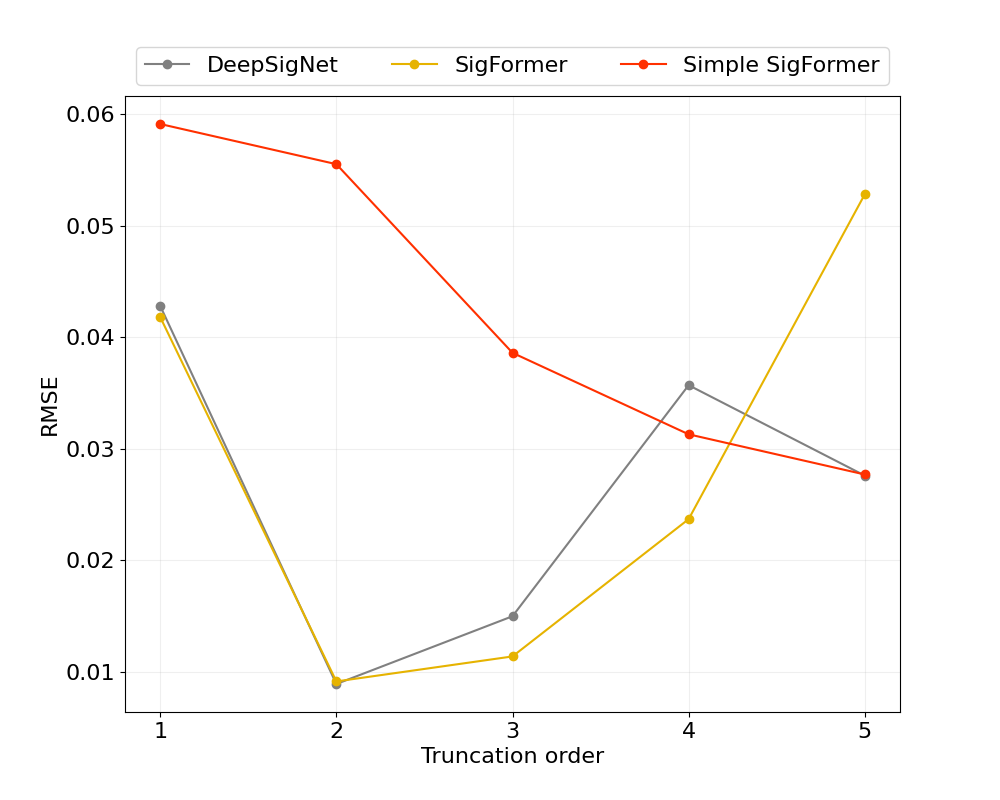
\includegraphics[width=0.32\textwidth]{fig//numerical_example2//example2_fBm.png}
		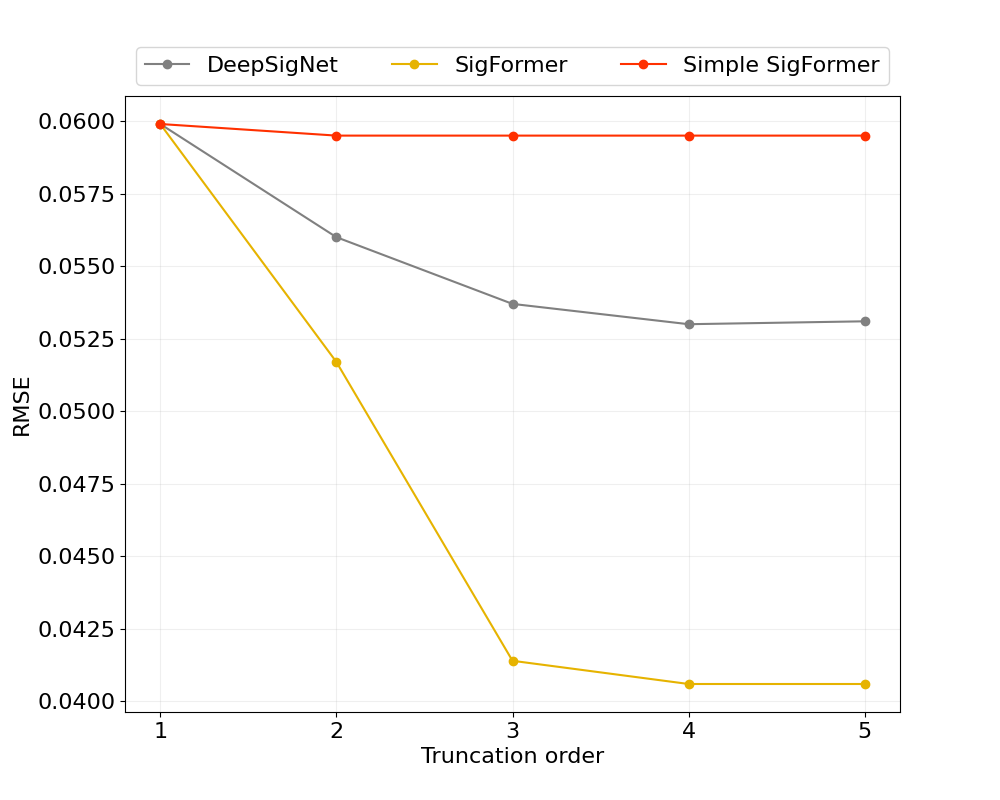
\includegraphics[width=0.32\textwidth]{fig//numerical_example2//example2_rBergomi.png}
		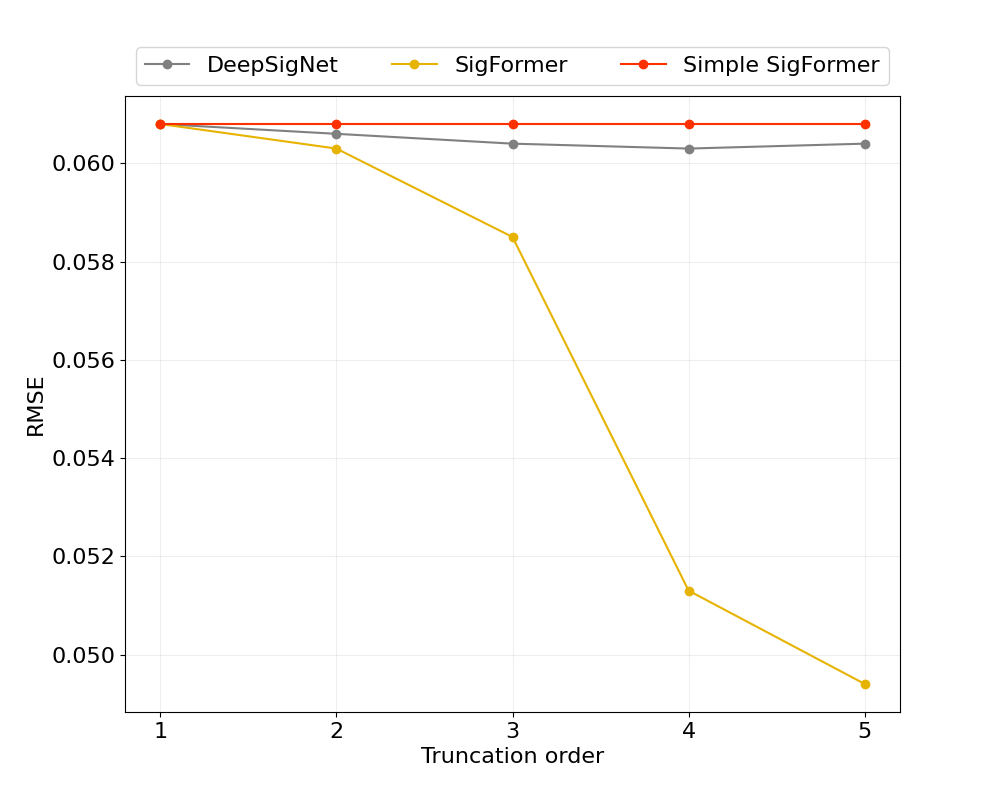
\includegraphics[width=0.32\textwidth]{fig//numerical_example2//example2_rHeston.png}
		\caption{RMSE of calibrating $H$  for different volatility models (Left: fBms; Middle: rBergomi volatility processes; Right: rHeston volatility processes), averaged over 3 training runs, over signature truncation order varying from $1$ to $5$.}
	\end{figure}
	
	\subsubsection{The effective of CNN and MLP in the SigFormer model}
	\label{subsubsec-sensitivity-structure}
	In this section, we want to explore the effective of CNN and MLP structure in the SigFormer model. Notice that the Remark 2 from~\cite{tong_2023} has mentioned that the transformer in their model can help to extract representations from signatures instead of using CNN. So we want to see whether the CNN and MLP in our SigFormer model matters to achieve higher accuracy.
	
	In order to validate the effective of both the convolutional and the fully connected layers in our SigFormer model, we propose another three simple signature-based transformer for comparison, the architecture of these three simple SigFormer models are presented in Appendix~\ref{subapdix-architecture-simplesignature}. And we also provide the Simple Sigformer model from Section~\ref{subsubsec-sensitivity-truncation} for reference. The results are shown in Table~\ref{tab-sensitivity-structure-uniform} for $H\sim\text{Uniform}(0,\,0.5)$ and Table~\ref{tab-sensitivity-structure-beta} for $H\sim\text{Beta}(1,\,9)$ with the corresponding loss plots shown in Appendix~\ref{subapdix-loss-plots-structure}. 
	
	From these results, we can easily find that the CNN and MLP structure in SigFormer model do help to achieve higher accuracy. The Remark 2 from~\cite{tong_2023} means that the transformer could be a better alternative for CNN and MLP in signature-based model. But they haven't discuss whether there is beneficial to combine CNN and MLP with transformer in signature-based model. From the results in Section~\ref{subsubsec-sensitivity-structure}, the CNN and MLP do help to achieve higher accuracy in our model. We put the CNN before taking signature and the transformer after taking signature, so they play different roles in our SigFormer model. The CNN may enhance the ability of signature transform to extract features from paths while the transformer is used to process the output. To realize the role of CNN in our model, we need to dive into the models' structures. We can observe that the dimension of output from signature transform are $[5,\,5^2,\,5^3]$ and $[2,\,2^2,\,2^3]$ for SigFormer with and without CNN respectively. This is because we employ a CNN with $3$ channels in the former one to increase the dimensionality of the original path with time (i.e. $2$ features to $5$ features). The MLP in our SigFormer model is used after the transformer. Without the MLP, we can observe some fluctuations during training processes presented in Appendix~\ref{subapdix-loss-plots-structure}. The MLP makes our SigFormer model more stable so as to achieve higher accuracy.
	
	\begin{table}[H]
		\caption{Test results for different SigFormer models, averaged over 3 training runs, with input lengths varying from $100$ to $300$ and $H\sim\text{Uniform}(0,\,0.5)$.}
		\label{tab-sensitivity-structure-uniform}
		\smallskip
		\centering
		\renewcommand\arraystretch{1.5}
		\resizebox{\textwidth}{!}{
			\begin{tabular}{l c c c c c}
				\toprule
				\multirow{2}{*}{Models}&\multirow{2}{*}{Input length}&\multicolumn{3}{c}{Test RMSE}&\multirow{2}{*}{$\#$Params}\\
				\cline{3-5}
				&&fBm&rBergomi&rHeston&\\
				\hline
				\multirow{3}{*}{SigFormer without CNN}
				&100&$5.36\times10^{-2}$&$1.43\times10^{-1}$&$1.42\times10^{-1}$&5647\\
				&200&$4.76\times10^{-2}$&$1.45\times10^{-1}$&$1.46\times10^{-1}$&6543\\
				&300&$4.68\times10^{-2}$&$1.47\times10^{-1}$&$1.43\times10^{-1}$&7439\\
				
				\hline
				\multirow{3}{*}{SigFormer without MLP}
				&100&$1.18\times10^{-1}$&$1.16\times10^{-1}$&$8.33\times10^{-2}$&73328\\
				&200&$1.45\times10^{-1}$&$1.12\times10^{-1}$&$6.31\times10^{-2}$&73638\\
				&300&$1.01$&$1.10\times10^{-1}$&$5.84\times10^{-2}$&73948\\
				
				\hline
				\multirow{3}{*}{SigFormer  without CNN and MLP}
				&100&$8.80\times10^{-2}$&$1.43\times10^{-1}$&$1.42\times10^{-1}$&491\\
				&200&$7.67\times10^{-2}$&$1.45\times10^{-1}$&$1.45\times10^{-1}$&519\\
				&300&$8.96\times10^{-2}$&$1.47\times10^{-1}$&$1.42\times10^{-1}$&547\\
				
				\hline
				\multirow{3}{*}{SigFormer}
				&100&$1.44\times10^{-2}$&$5.35\times10^{-2}$&$8.43\times10^{-2}$&87226\\
				&200&$1.42\times10^{-2}$&$4.74\times10^{-2}$&$7.10\times10^{-2}$&97146\\
				&300&$1.55\times10^{-2}$&$4.51\times10^{-2}$&$6.29\times10^{-2}$&107066\\
				
				\hline
				\multirow{3}{*}{Simple SigFormer}
				&100&$7.18\times10^{-2}$&$1.43\times10^{-1}$&$1.43\times10^{-1}$&6666\\
				&200&$6.55\times10^{-2}$&$1.45\times10^{-1}$&$1.47\times10^{-1}$&6666\\
				&300&$6.77\times10^{-2}$&$1.47\times10^{-1}$&$1.44\times10^{-1}$&6666\\
				
				\bottomrule	
			\end{tabular}
		}
	\end{table}
	
	\begin{table}[H]
		\caption{Test results for different SigFormer models, averaged over 3 training runs, with input lengths varying from $100$ to $300$ and $H\sim\text{Beta}(1,\,9)$.}
		\label{tab-sensitivity-structure-beta}
		\smallskip
		\centering
		\renewcommand\arraystretch{1.5}
		\resizebox{\textwidth}{!}{
			\begin{tabular}{l c c c c c}
				\toprule
				\multirow{2}{*}{Models}&\multirow{2}{*}{Input length}&\multicolumn{3}{c}{Test RMSE}&\multirow{2}{*}{$\#$Params}\\
				\cline{3-5}
				&&fBm&rBergomi&rHeston&\\
				\hline
				\multirow{3}{*}{SigFormer without CNN}
				&100&$2.53\times10^{-2}$&$6.12\times10^{-2}$&$5.94\times10^{-2}$&5647\\
				&200&$2.43\times10^{-2}$&$5.91\times10^{-2}$&$5.96\times10^{-2}$&6543\\
				&300&$2.21\times10^{-2}$&$5.90\times10^{-2}$&$5.83\times10^{-2}$&7439\\
				
				\hline
				\multirow{3}{*}{SigFormer without MLP}
				&100&$1.25\times10^{-1}$&$5.02\times10^{-2}$&$3.98\times10^{-2}$&73328\\
				&200&$6.09\times10^{-1}$&$4.33\times10^{-2}$&$2.35\times10^{-2}$&73638\\
				&300&$1.08$&$4.49\times10^{-2}$&$2.17\times10^{-2}$&73948\\
				
				\hline
				\multirow{3}{*}{SigFormer  without CNN and MLP}
				&100&$4.34\times10^{-2}$&$6.12\times10^{-2}$&$5.91\times10^{-2}$&491\\
				&200&$4.78\times10^{-2}$&$5.91\times10^{-2}$&$5.94\times10^{-2}$&519\\
				&300&$4.66\times10^{-2}$&$5.90\times10^{-2}$&$5.82\times10^{-2}$&547\\
				
				\hline
				\multirow{3}{*}{SigFormer}
				&100&$1.14\times10^{-2}$&$4.18\times10^{-2}$&$5.76\times10^{-2}$&87226\\
				&200&$1.19\times10^{-2}$&$3.64\times10^{-2}$&$5.56\times10^{-2}$&97146\\
				&300&$1.13\times10^{-2}$&$3.24\times10^{-2}$&$5.03\times10^{-2}$&107066\\
				
				\hline
				\multirow{3}{*}{Simple SigFormer}
				&100&$4.07\times10^{-2}$&$6.12\times10^{-2}$&$5.94\times10^{-2}$&6666\\
				&200&$3.53\times10^{-2}$&$5.91\times10^{-2}$&$5.97\times10^{-2}$&6666\\
				&300&$3.46\times10^{-2}$&$5.91\times10^{-2}$&$5.84\times10^{-2}$&6666\\
				
				\bottomrule	
			\end{tabular}
		}
	\end{table}
	
	Furthermore, we also want to verify the effective of CNN and MLP in multiple parameters calibration problems. Hence, we sample $\theta\sim\text{Uniform}(0,\,0.5)$\footnote{The corresponding set of possible $\theta$ values is $\{0.05,\,0.14,\,0.21,\,0.30,\,0.42\}$.} as well as $H\sim\text{Beta}(1,\,9)$ to generate rough Heston volatility paths as Section~\ref{subsubsec-sensitivity-implementation}. The results are shown in Table~\ref{tab-sensitivity-structure-multiple} with the corresponding loss plots shown in Appendix~\ref{subapdix-loss-plots-structure}. The analysis of the single calibration problem also applies here.
	\begin{table}[H]
		\caption{Test results for different SigFormer models, averaged over 3 training runs, with input lengths varying from $100$ to $300$. Here, $H\sim\text{Beta}(1,\,9)$ and $\theta\sim\text{Uniform}(0,\,0.5)$.}
		\label{tab-sensitivity-structure-multiple}
		\smallskip
		\centering
		\renewcommand\arraystretch{1.5}
		\resizebox{\textwidth}{!}{
			\begin{tabular}{l c c c}
				\toprule
				Models&Input length&Test RMSE&$\#$Params\\
				\hline
				\multirow{3}{*}{SigFormer without CNN}
				&100&$9.64\times10^{-2}$&5680\\
				&200&$9.78\times10^{-2}$&6576\\
				&300&$9.77\times10^{-2}$&7472\\
				
				\hline
				\multirow{3}{*}{SigFormer without MLP}
				&100&$4.98\times10^{-2}$&73639\\
				&200&$5.11\times10^{-2}$&74259\\
				&300&$4.90\times10^{-2}$&74879\\
				
				\hline
				\multirow{3}{*}{SigFormer  without CNN and MLP}
				&100&$7.94\times10^{-2}$&520\\
				&200&$5.94\times10^{-2}$&576\\
				&300&$8.06\times10^{-2}$&632\\
				
				\hline
				\multirow{3}{*}{SigFormer}
				&100&$4.99\times10^{-2}$&87259\\
				&200&$5.10\times10^{-2}$&97179\\
				&300&$5.18\times10^{-2}$&107099\\
				
				\hline
				\multirow{3}{*}{Simple SigFormer}
				&100&$9.94\times10^{-2}$&6822\\
				&200&$1.00\times10^{-1}$&6822\\
				&300&$9.98\times10^{-2}$&6822\\
				
				\bottomrule	
			\end{tabular}
		}
	\end{table}

	\subsection{Calibrating the Hurst parameter from rough volatility paths with different lengths}
	\label{subsec-single-calibration}
	Estimating the Hurst parameter $H$ of a fBm, rBergomi or rHeston path is considered a nontrivial task because of the paths’ non-stationarity and long range dependencies. Therefore paths with more time steps and smaller $H$ (i.e. rougher) are more difficult to calibrate. 
	
	In this example, we train a variety of models that we mentioned before to perform this estimation. That is, to learn the map $(t^n,\,X^n)\mapsto H$, where $t^n$ denotes the time steps and $X^n$ are the corresponding simulated paths. We use paths from Section~\ref{subsubsec-sensitivity-implementation} with the number of time steps varying from $100$ to $500$ and all other settings are the same as illustrated in Section~\ref{subsubsec-sensitivity-implementation}.
		
	The results are shown in Table~\ref{tab-calibration-single-uniform} for $H\sim\text{Uniform}(0,\,0.5)$ and Table~\ref{tab-calibration-single-beta} for $H\sim\text{Beta}(1,\,9)$ with the corresponding loss plots shown in Appendix~\ref{subapdix-loss-plots-calibration-single}. In order to present the results more clearly, we also plot Table~\ref{tab-calibration-single-uniform} and Table~\ref{tab-calibration-single-beta} into Figure~\ref{fig-calibration-single}. 
	From these results, we can easily conclude that the SigFormer model tends to outperform the competing models in three scenarios for single parameter calibration problems: (a) paths with more time steps; (b) rougher paths; (c) paths simulated by more complex volatility models. We attribute this to the self-attention mechanism, which enhances the capacity of the SigFormer model for analyzing information from path signatures, thereby making it outperforming in complex calibration problems. 
	We also observe that the number of parameters i.e. the complexity for the SigFormer model increases with the input length while the DeepSigNet model maintain a constant number of parameters. This feature of the SigFormer model is not directly from introducing the multi-head self-attention layer, but rather through the lifting operation before taking the signature. We also notice that the transformer model has better accuracy than our SigFormer model in some cases. But the transformer model is more complex than our SigFormer model.
	
	\begin{table}[H]
		\caption{Test results for different models, averaged over 3 training runs, with input lengths varying from $100$ to $500$ and $H\sim\text{Uniform}(0,\,0.5)$.}
		\label{tab-calibration-single-uniform}
		\smallskip
		\centering
		\renewcommand\arraystretch{1.5}
		\resizebox{\textwidth}{!}{
			\begin{tabular}{l c c c c c}
				\toprule
				\multirow{2}{*}{Models}&\multirow{2}{*}{Input length}&\multicolumn{3}{c}{Test RMSE}&\multirow{2}{*}{$\#$Params}\\
				\cline{3-5}
				&&fBm&rBergomi&rHeston&\\
				\hline
				\multirow{5}{*}{Transformer}
				&100&$8.05\times10^{-3}$&$5.79\times10^{-2}$&$8.82\times10^{-2}$&573906\\
				&200&$6.07\times10^{-3}$&$4.86\times10^{-2}$&$8.00\times10^{-2}$&1069906\\
				&300&$6.78\times10^{-3}$&$5.04\times10^{-2}$&$9.55\times10^{-2}$&1565906\\
				&400&$7.53\times10^{-3}$&$3.76\times10^{-2}$&$8.67\times10^{-2}$&2061906\\
				&500&$1.11\times10^{-2}$&$4.61\times10^{-2}$&$8.17\times10^{-2}$&2557906\\
				\hline
				\multirow{5}{*}{SigFormer}
				&100&$1.36\times10^{-2}$&$5.38\times10^{-2}$&$9.06\times10^{-2}$&87226\\
				&200&$1.54\times10^{-2}$&$4.95\times10^{-2}$&$6.99\times10^{-2}$&97146\\
				&300&$1.56\times10^{-2}$&$4.28\times10^{-2}$&$5.49\times10^{-2}$&107066\\
				&400&$1.90\times10^{-2}$&$3.79\times10^{-2}$&$5.47\times10^{-2}$&116986\\
				&500&$1.43\times10^{-2}$&$3.88\times10^{-2}$&$4.36\times10^{-2}$&126906\\
				\hline
				\multirow{5}{*}{DeepSigNet}
				&100&$1.69\times10^{-2}$&$6.22\times10^{-2}$&$1.31\times10^{-1}$&9261\\
				&200&$1.69\times10^{-2}$&$5.38\times10^{-2}$&$1.25\times10^{-1}$&9261\\
				&300&$1.62\times10^{-2}$&$4.29\times10^{-2}$&$1.27\times10^{-1}$&9261\\
				&400&$2.09\times10^{-2}$&$4.50\times10^{-2}$&$1.22\times10^{-1}$&9261\\
				&500&$1.81\times10^{-2}$&$4.31\times10^{-2}$&$1.20\times10^{-1}$&9261\\
				\hline
				\multirow{5}{*}{CNN}
				&100&$7.24\times10^{-2}$&$5.11\times10^{-2}$&$9.56\times10^{-2}$&255073\\
				&200&$8.42\times10^{-2}$&$4.79\times10^{-2}$&$8.73\times10^{-2}$&320609\\
				&300&$8.66\times10^{-2}$&$5.51\times10^{-2}$&$9.82\times10^{-2}$&386145\\
				&400&$7.76\times10^{-2}$&$4.84\times10^{-2}$&$9.21\times10^{-2}$&435297\\
				&500&$8.51\times10^{-2}$&$4.31\times10^{-2}$&$8.86\times10^{-2}$&500833\\
				\bottomrule	
			\end{tabular}
		}
	\end{table}
	
	\begin{table}[H]
		\caption{Test results for different models, averaged over 3 training runs, with input lengths varying from $100$ to $500$ and $H\sim\text{Beta}(1,\,9)$.}
		\label{tab-calibration-single-beta}
		\smallskip
		\centering
		\renewcommand\arraystretch{1.5}
		\resizebox{\textwidth}{!}{
			\begin{tabular}{l c c c c c}
				\toprule
				\multirow{2}{*}{Models}&\multirow{2}{*}{Input length}&\multicolumn{3}{c}{Test RMSE}&\multirow{2}{*}{$\#$Params}\\
				\cline{3-5}
				&&fBm&rBergomi&rHeston&\\
				\hline
				\multirow{5}{*}{Transformer}
				&100&$8.97\times10^{-3}$&$5.02\times10^{-2}$&$6.04\times10^{-2}$&573906\\
				&200&$9.43\times10^{-3}$&$4.02\times10^{-2}$&$5.73\times10^{-2}$&1069906\\
				&300&$1.15\times10^{-2}$&$3.25\times10^{-2}$&$5.78\times10^{-2}$&1565906\\
				&400&$7.96\times10^{-3}$&$3.21\times10^{-2}$&$5.82\times10^{-2}$&2061906\\
				&500&$8.05\times10^{-3}$&$2.60\times10^{-2}$&$5.86\times10^{-2}$&2557906\\
				\hline
				\multirow{5}{*}{SigFormer}
				&100&$1.28\times10^{-2}$&$3.92\times10^{-2}$&$5.81\times10^{-2}$&87226\\
				&200&$1.78\times10^{-2}$&$3.36\times10^{-2}$&$5.63\times10^{-2}$&97146\\
				&300&$1.93\times10^{-2}$&$2.87\times10^{-2}$&$3.35\times10^{-2}$&107066\\
				&400&$1.48\times10^{-2}$&$3.13\times10^{-2}$&$2.91\times10^{-2}$&116986\\
				&500&$1.75\times10^{-2}$&$2.79\times10^{-2}$&$3.13\times10^{-2}$&126906\\
				\hline
				\multirow{5}{*}{DeepSigNet}
				&100&$1.64\times10^{-2}$&$5.18\times10^{-2}$&$6.03\times10^{-2}$&9261\\
				&200&$1.49\times10^{-2}$&$4.42\times10^{-2}$&$5.82\times10^{-2}$&9261\\
				&300&$1.66\times10^{-2}$&$4.23\times10^{-2}$&$5.76\times10^{-2}$&9261\\
				&400&$1.73\times10^{-2}$&$3.70\times10^{-2}$&$5.89\times10^{-2}$&9261\\
				&500&$2.14\times10^{-2}$&$3.56\times10^{-2}$&$5.80\times10^{-2}$&9261\\
				\hline
				\multirow{5}{*}{CNN}
				&100&$1.30\times10^{-1}$&$5.69\times10^{-2}$&$8.45\times10^{-2}$&255073\\
				&200&$1.10\times10^{-1}$&$6.15\times10^{-2}$&$8.47\times10^{-2}$&320609\\
				&300&$8.80\times10^{-2}$&$5.59\times10^{-2}$&$8.44\times10^{-2}$&386145\\
				&400&$8.76\times10^{-2}$&$5.77\times10^{-2}$&$7.93\times10^{-2}$&435297\\
				&500&$8.37\times10^{-2}$&$5.84\times10^{-2}$&$8.09\times10^{-2}$&500833\\
				\bottomrule	
			\end{tabular}
		}
	\end{table}
	
	\begin{figure}[H]
		\centering
		\resizebox{0.9\textwidth}{!}{
			\subfigure[$H\sim\text{Uniform}(0,0.5)$]{
				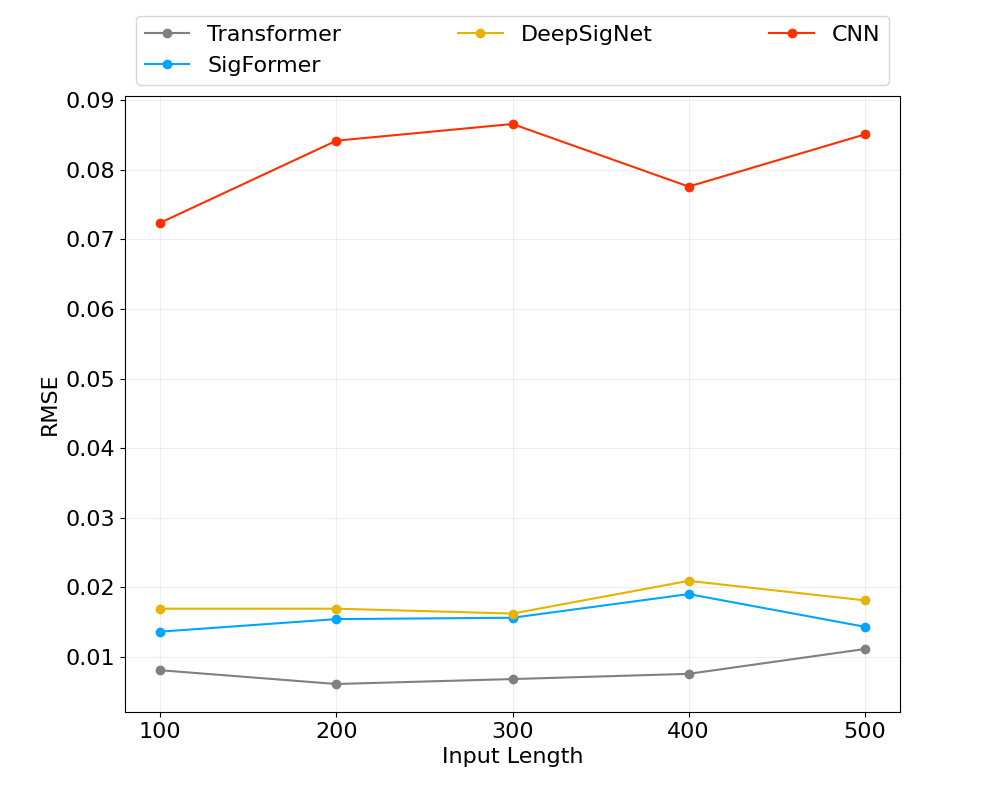
\includegraphics[width=0.32\textwidth]{fig//numerical_example4//example4_Huniform_fBm.png}
				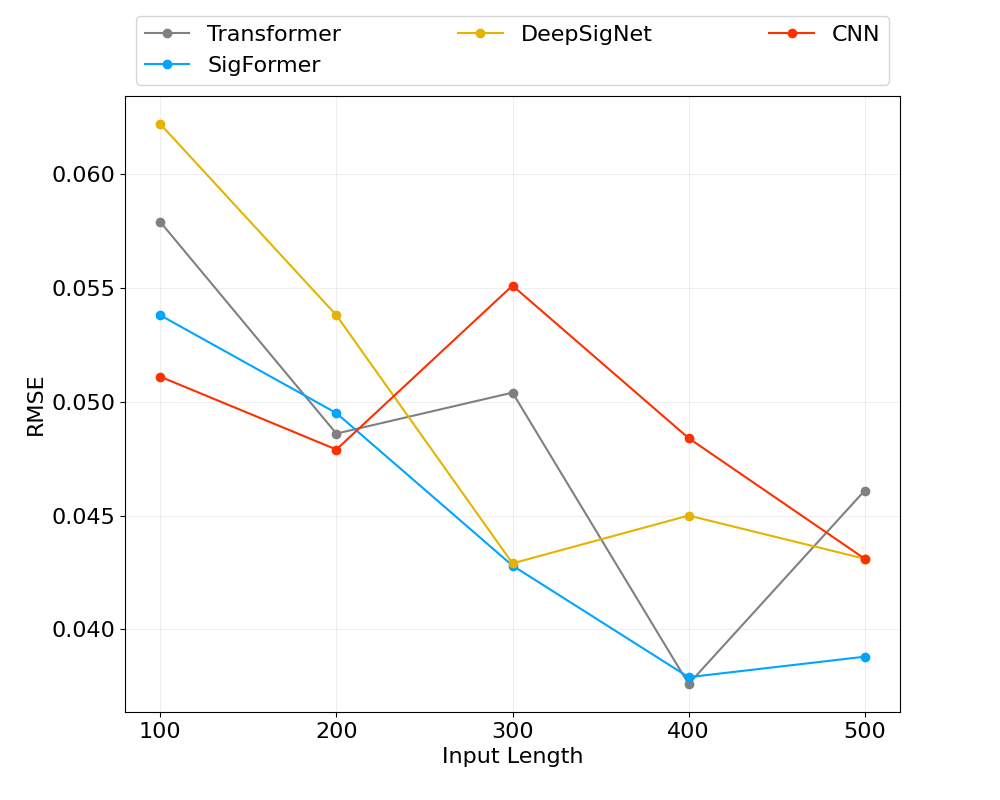
\includegraphics[width=0.32\textwidth]{fig//numerical_example4//example4_Huniform_rBergomi.png}
				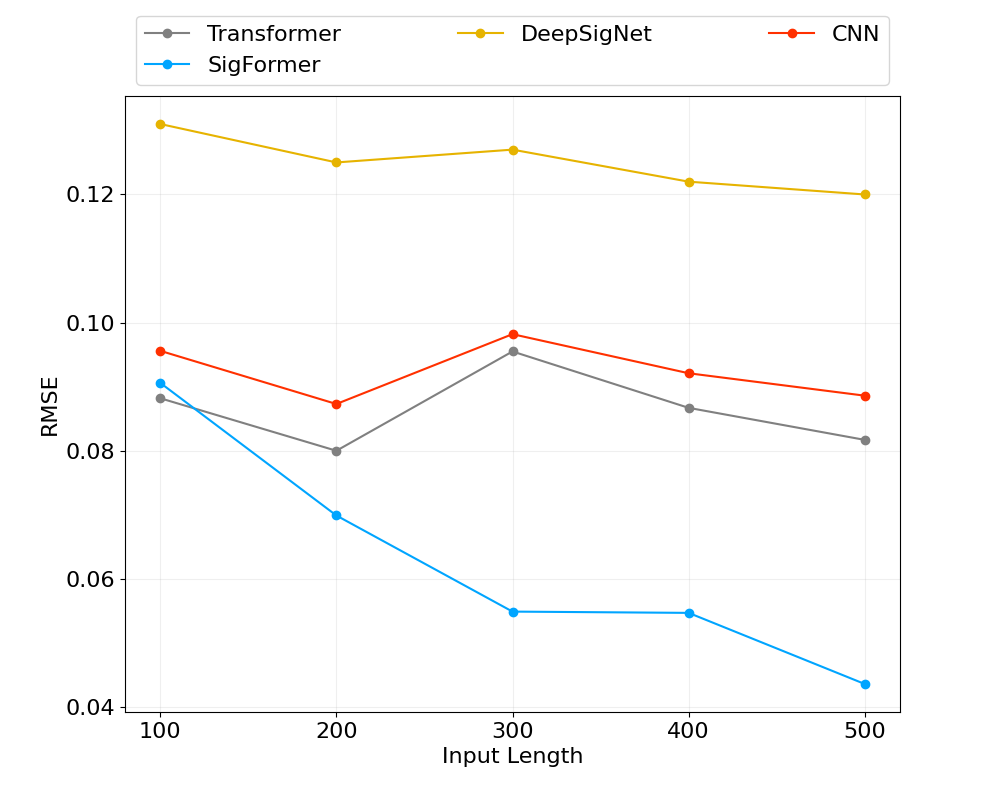
\includegraphics[width=0.32\textwidth]{fig//numerical_example4//example4_Huniform_rHeston.png}}
		}
		\resizebox{0.9\textwidth}{!}{
			\subfigure[$H\sim\text{Beta}(1,\,9)$]{
				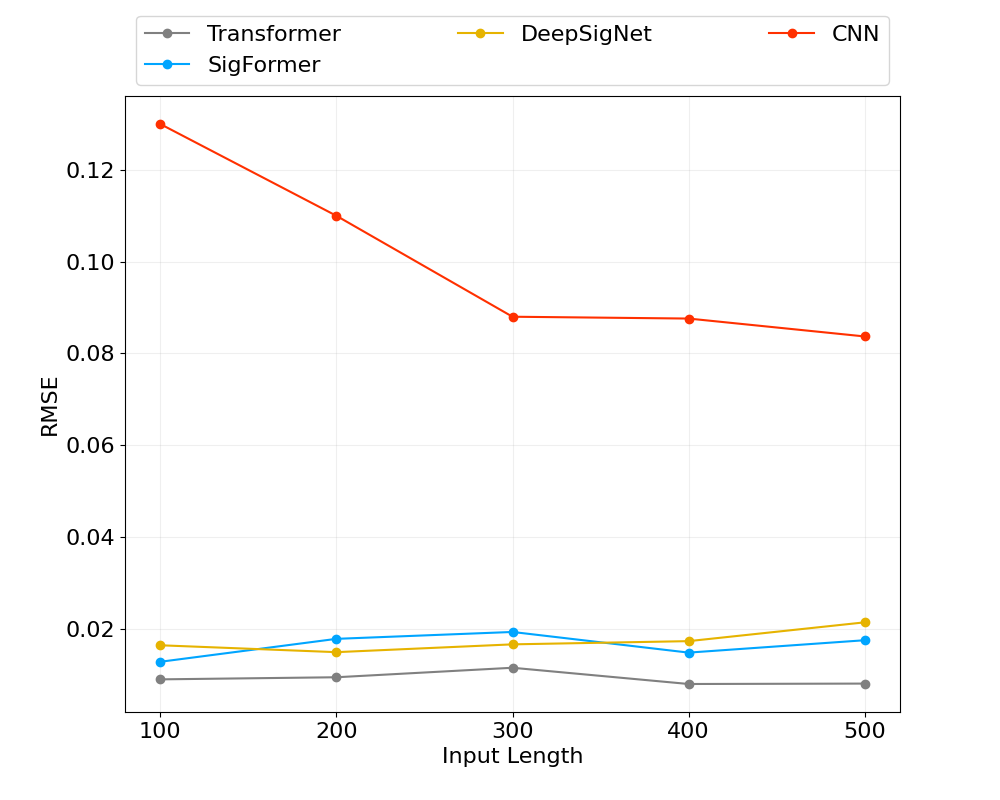
\includegraphics[width=0.32\textwidth]{fig//numerical_example4//example4_Hbeta_fBm.png}
				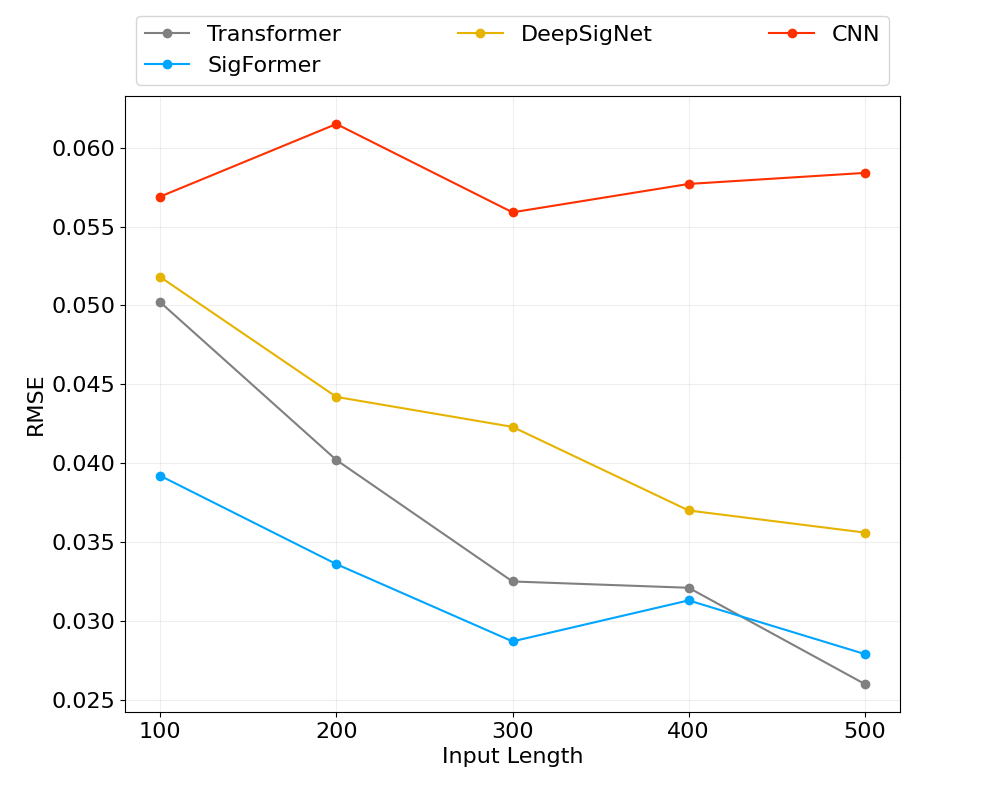
\includegraphics[width=0.32\textwidth]{fig//numerical_example4//example4_Hbeta_rBergomi.png}
				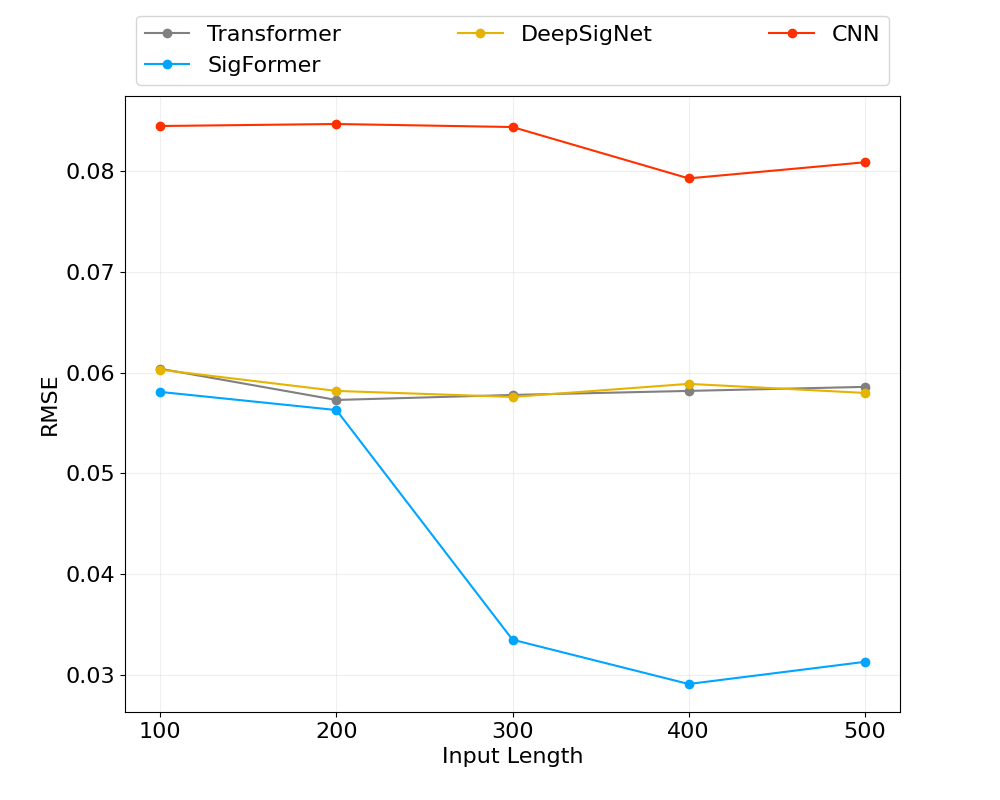
\includegraphics[width=0.32\textwidth]{fig//numerical_example4//example4_Hbeta_rHeston.png}}
		}
		\caption{RMSE of calibrating $H$  for different volatility models (Left: fBms; Middle: rBergomi volatility processes; Right: rHeston volatility processes) over input lengths vary from $100$ to $500$. }
		\label{fig-calibration-single}
	\end{figure}
	
	\subsection{Calibrating multiple parameters with rough volatility processes}
	\label{subsec-multiple}
	In previous examples, we have observed that the SigFormer model tends to outperform competing models in many complex calibration problems, such as those involving paths simulated by advanced volatility models and more time steps. Therefore, it is natural to consider applying the SigFormer model in multiple parameters calibration problems. 
	
	\subsubsection{Implementation details}
	\label{subsubsec-multiple-implementation}
	In order to generate the data sets for multiple parameters calibration problems, we first sample different $\eta,\kappa_1,\,\kappa_2,\,\theta$ from the distribution shown in Table~\ref{tab-multiple-distribution}. Then we simulate rBergomi and rHeston paths with these parameters, as well as $H\sim\text{Beta}(1,\,9)$, from Section~\ref{subsubsec-sensitivity-implementation} to generate two corresponding training/test data sets with the same size as shown in Table~\ref{tab-data-size} and all paths are simulated $100$ steps. The first data set consists of rBergomi paths with different $\eta$ and $H$. The second data set consists of rHeston paths with different $\kappa_1,\,\kappa_2,\,\theta$ and $H$. All other settings are kept the same as Section~\ref{subsubsec-sensitivity-implementation}.
	\begin{table}[H]
		\caption{Distributions for sampling parameters.}
		\label{tab-multiple-distribution}
		\smallskip
		\centering
		\renewcommand\arraystretch{1.5}
		\begin{tabular}{l c c}
			\toprule
			Parameters&Distributions&Values\\
			\hline
			$\eta$&$\text{Uniform}(0,\,3)$&$\{0.41,\,1.04,\,1.56,\,2.40,\,2.73\}$\\
			$\kappa_1$&$\text{Uniform}(0,\,5)$&$\{0.25,\,1.24,\,2.83,\,3.02,\,4.81\}$\\
			$\kappa_2$&$\text{Uniform}(0,\,3)$&$\{0.13,\,0.79,\,1.58,\,2.23,\,2.94\}$\\
			$\theta$&$\text{Uniform}(0,\,0.5)$&$\{0.05,\,0.14,\,0.21,\,0.30,\,0.42\}$\\
			\bottomrule
		\end{tabular}
	\end{table}
	
	\subsubsection{Multiple parameters calibration}
	\label{subsubsec-multiple-calibration}
	We begin this section by calibrating two parameters simultaneously: $H,\,\eta$ of rBergomi volatility processes and we also perform four parameters calibrations for rHeston volatility processes (i.e. $H,\,\kappa_1,\,\kappa_2$ and $\theta$). The results are shown in Table~\ref{tab-multiple-two} with the corresponding loss plots shown in Appendix~\ref{subapdix-loss-plots-calibration-multiple}.
	
	\begin{table}[H]
		\caption{Test results for multiple parameters calibration with $H\sim\text{Beta}(1,\,9)$, $\eta\sim\text{Uniform}(0,\,3)$, $\kappa_1\sim\text{Uniform}(0,\,5)$, $\kappa_2\sim\text{Uniform}(0,\,3)$ and $\theta\sim\text{Uniform}(0,\,0.5)$.}
		\label{tab-multiple-two}
		\smallskip
		\centering
		\renewcommand\arraystretch{1.5}
		\begin{tabular}{l c c | c c}
			\toprule
			Models&RMSE of rBergomi&Params&RMSE of rHeston&Params\\
			\hline
			Transformer&0.448&573939&0.689&574005\\
			\hline
			SigFormer&0.289&87259&0.672&87325\\
			\hline
			DeepSigNet&0.564&9294&0.769&9360\\
			\hline
			CNN&0.388&255202&0.768&255460\\
			\bottomrule
		\end{tabular}
	\end{table}
	
	 In these multiple calibration problems, we observe that our SigFormer model achieves the best accuracy. And we also notice that models with transformer achieve better accuracy than those without. These results further demonstrate the advantages of combining self-attention mechanism with the signature transform for calibrating complex rough paths.
		
	\subsection{Empirical studies}
	\label{subsec-empirical}
	In this example, we follow \cite{stone_2020} to calibrate the H$\ddot{\rm o}$lder exponent of historic realised volatility data from the Oxford–Man Institute of Quantitative Finance. We generate the training and evaluation data sets by the rough Heston model with two different Hurst parameters i.e. $H\sim\text{Beta}(1,\,9)$ and $H\sim\text{Uniform}(0,\,0.5)$ as illustrated in Section~\ref{subsubsec-sensitivity-implementation}. We choose the length of the input vectors to be $100$. We took a sample of $10$ different indices; for each index we then used a time series of $200$ sequential data points to create $11$ vectors of length $100$ (entries $0$ to $100$, $10$ to $110$ and so on) to predict the H$\ddot{\rm o}$lder exponent for each index. We compute the RMSE between the models' predictions and the least square prediction, and the standard deviation of the difference between these predictions, see Table~\ref{tab-empirical}. We also present the loss plots for training in Appendix~\ref{subapdix-loss-plots-empirical}. We notice that models trained with $H\sim\text{Beta}(1,\,9)$ achieve better accuracy than those who trained with $H\sim\text{Uniform}(0,\,0.5)$. This means that the log-volatility behaves essentially as a fBm with Hurst exponent $H$ of order $0.1$, at any reasonable time scale.
	
		\begin{table}[H]
		\caption{Calibration results for different models with $H\sim\text{Beta}(1,\,9)$ and $H\sim\text{Uniform}(0,\,0.5)$.}
		\label{tab-empirical}
		\smallskip
		\centering
		\renewcommand\arraystretch{1.5}
		\begin{tabular}{l c c c}
			\toprule
			\multirow{2}{*}{Models}&\multicolumn{2}{c}{RMSE (Standard deviation)}&\multirow{2}{*}{$\#$Params}\\
			\cline{2-3}
			&$H\sim\text{Uniform}(0,\,0.5)$&$H\sim\text{Beta}(1,\,9)$&\\
			\hline
			SigFormer&0.285($9.30\times10^{-3}$)&0.016($6.09\times10^{-4}$)&87226\\
			\hline
			DeepSigNet&0.152($5.16\times10^{-3}$)&0.032($5.23\times10^{-4}$)&9261\\
			\hline
			CNN&0.776($2.46\times10^{-2}$)&0.045($1.75\times10^{-3}$)&255073\\
			\hline
			Simple SigFormer&0.095($3.34\times10^{-3}$)&0.038($7.11\times10^{-4}$)&6822\\
			\hline
			Transformer&0.221($7.36\times10^{-3}$)&0.026($3.50\times10^{-4}$)&573906\\
			\bottomrule
		\end{tabular}
	\end{table}
	
	\section{Conclusion}
	\label{sec-conclusion}
	There is a solid theoretical ground for using the signature transform as a tool to calibrate the streams of data. Meanwhile transformers have enjoyed great empirical success in handling sequential data. It is thus natural to combine them together to calibrate volatility processes; in this paper we have constructed a SigFormer model to present how to do this, and also have provided examples to explore the performance of the SigFormer model in different calibration problems.
	
	There are two main contributions in this paper. First, we give the way to combine the signature transform with the self-attention mechanism. Second, we present how to specify the details of the SigFormer model as well as how to simplify it without substantially compromising accuracy.
	%%%%%%%%%%%%%%%%%%%%%%%%%%%%%%%%%%%%%%%%%%%%%%%%%%
	
	%References
	\printbibliography
	
	
	
	%%%%%%%%%%%%%%%%%%%%%%%%%%%%%%%%%%%%%%%%%%%%%%%%%%
	\appendix
	\section{Architecture of different models}
	\label{apdix-architecture}
	\subsection{Architecture of the CNN, DeepSigNet and transformer model}
	\label{subapdix-architecture-cnndeepsignettransform}
	Here we clarify the specific architecture of CNN, DeepSigNet and transformer model as below:
	\begin{itemize}
		\item The architecture of CNN model:
		\begin{itemize}
			\item[-] a convolutional layer with 32 channels and kernel size 20;
			\item[-] the leaky ReLu transform with negative slope 0.1;
			\item[-] a max pooling layer with size 3;
			\item[-] a dropout layer with rate 0.25;			
			\item[-] a convolutional layer with 64 channels and kernel size 20;
			\item[-] the leaky ReLu transform with negative slope 0.3;
			\item[-] a max pooling layer with size 3;
			\item[-] a dropout layer with rate 0.25;
			\item[-] a convolutional layer with 128 channels and kernel size 20;
			\item[-] the leaky ReLu transform with negative slope 0.1;
			\item[-] a max pooling layer with size 3;
			\item[-] a dropout layer with rate 0.4;
			\item[-] a dense layer with 128 units;
			\item[-] the leaky ReLu transform with negative slope 0.1;
			\item[-] a dropout layer with rate 0.3;
			\item[-] a dense layer with 1 units;
			\item[-] a non-linear transform with sigmoid function.			
		\end{itemize}
		\item The architecture of DeepSigNet model:
		\begin{itemize}
			\item[-] a convolutional layer with 3 channels and kernel size 3;
			\item[-] augmented with time and original values;
			\item[-] taking the signature transform with truncation order $N=3$;
			\item[-] a fully connected feedforward neural network with 5 hidden layers, each of size 32 and ReLU activation;
			\item[-] a non-linear transform with sigmoid function.
		\end{itemize}
		\item The architecture of transformer model:
		\begin{itemize}
			\item[-] a convolutional layer with 3 channels and kernel size 3;
			\item[-] augmented with time and original values;
			\item[-] a multi-head self-attention layer with the number of heads $h=N=3$;
			\item[-] a fully connected feedforward neural network with 5 hidden layers, each of size 32 and ReLU activation;
			\item[-] a non-linear transform with sigmoid function.
		\end{itemize}
	\end{itemize}
	\subsection{Architecture of simple signature-based transformer models}
	\label{subapdix-architecture-simplesignature}
	Here we clarify the specific architecture of different SigFormer models as below:
	\begin{itemize}
		\item The architecture of simple SigFormer model:
		\begin{itemize}
			\item[-] augmented with time;
			\item[-] taking the signature transform with truncation order $N=3$;
			\item[-] a single-head self-attention layer;
			\item[-] a non-linear transform with sigmoid function.
		\end{itemize}
		\item The architecture of SigFormer without CNN:
		\begin{itemize}
			\item[-] augmented with time;
			\item[-] taking the signature transform with truncation order $N=3$;
			\item[-] the multi-head self-attention layer with the number of heads $h=N=3$ and each different head corresponds to a different signature level;
			\item[-] a fully connected feedforward neural network with 5 hidden layers, each of size 32 and ReLU activation;			
			\item[-] a non-linear transform with sigmoid function.			
		\end{itemize}
		\item The architecture of SigFormer without MLP:
		\begin{itemize}
			\item[-] a convolutional layer with 3 channels and kernel size 3;
			\item[-] augmented with time and original values;
			\item[-] taking the signature transform with truncation order $N=3$;
			\item[-] the multi-head self-attention layer with the number of heads $h=N=3$ and each different head corresponds to a different signature level;
			\item[-] a linear transform to appropriate dimension.
		\end{itemize}
		\item The architecture of SigFormer without CNN and MLP:
		\begin{itemize}
			\item[-] augmented with time;
			\item[-] taking the signature transform with truncation order $N=3$;
			\item[-] the multi-head self-attention layer with the number of heads $h=N=3$ and each different head corresponds to a different signature level;
			\item[-] a linear transform to appropriate dimension.
		\end{itemize}
	\end{itemize}
	
	\section{Loss plots}
	\label{apdix-loss-plots}
	Here we present the loss plots for a particular (typical) training run since we have $3$ training runs for each experiment. And the data in loss plots has been taken the rolling mean with a window size of 5.
	
	\subsection{Loss plots for the SigFormer model with the stride varying from $1$ to $100$}
	\label{subapdix-loss-plots-stride}
	\begin{figure}[H]
		\centering
		\resizebox{0.9\textwidth}{!}{
			\subfigure[$H\sim\text{Uniform}(0,0.5)$]{
				
\includegraphics[width=0.32\textwidth]{fig//numerical_example1//loss_plots//fBm_grid=100_Huniform.eps}
				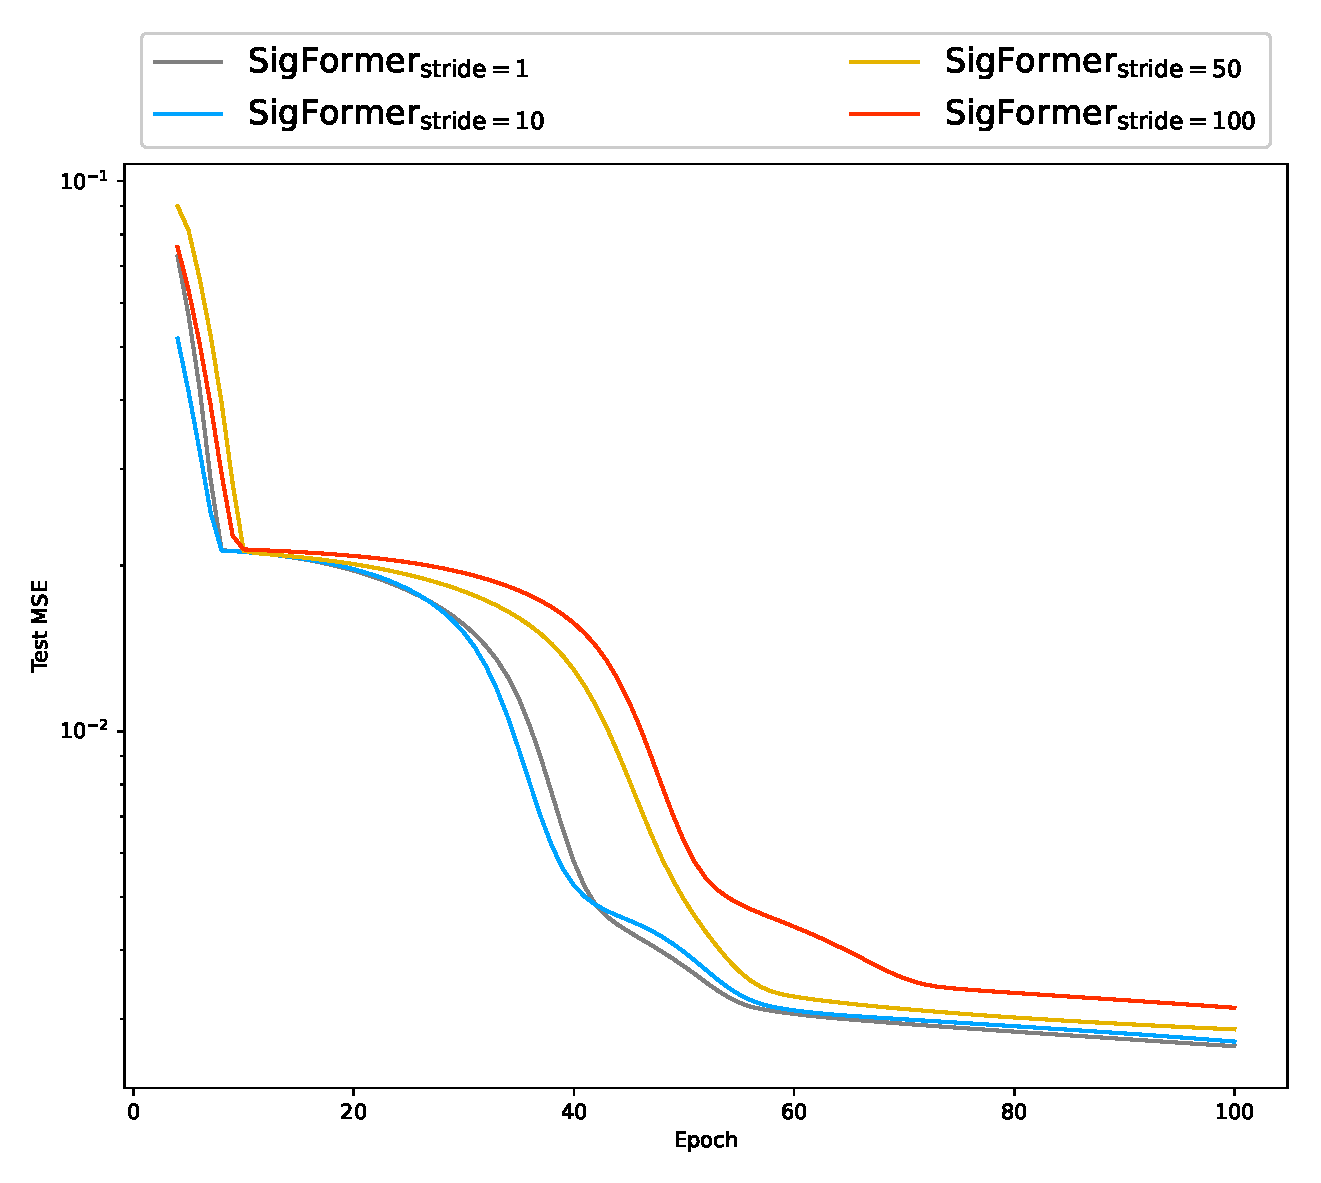
\includegraphics[width=0.32\textwidth]{fig//numerical_example1//loss_plots//rBergomi_grid=100_Huniform_eta=1_v0=0.01.eps}
				
\includegraphics[width=0.32\textwidth]{fig//numerical_example1//loss_plots//rHeston_grid=100_Huniform_kappa1=0.1_kappa2=0.03_theta=0.3_v0=0.01.eps}}
		}
		\resizebox{0.9\textwidth}{!}{
			\subfigure[$H\sim\text{Beta}(1,\,9)$]{
				
\includegraphics[width=0.32\textwidth]{fig//numerical_example1//loss_plots//fBm_grid=100_Hbeta.eps}
				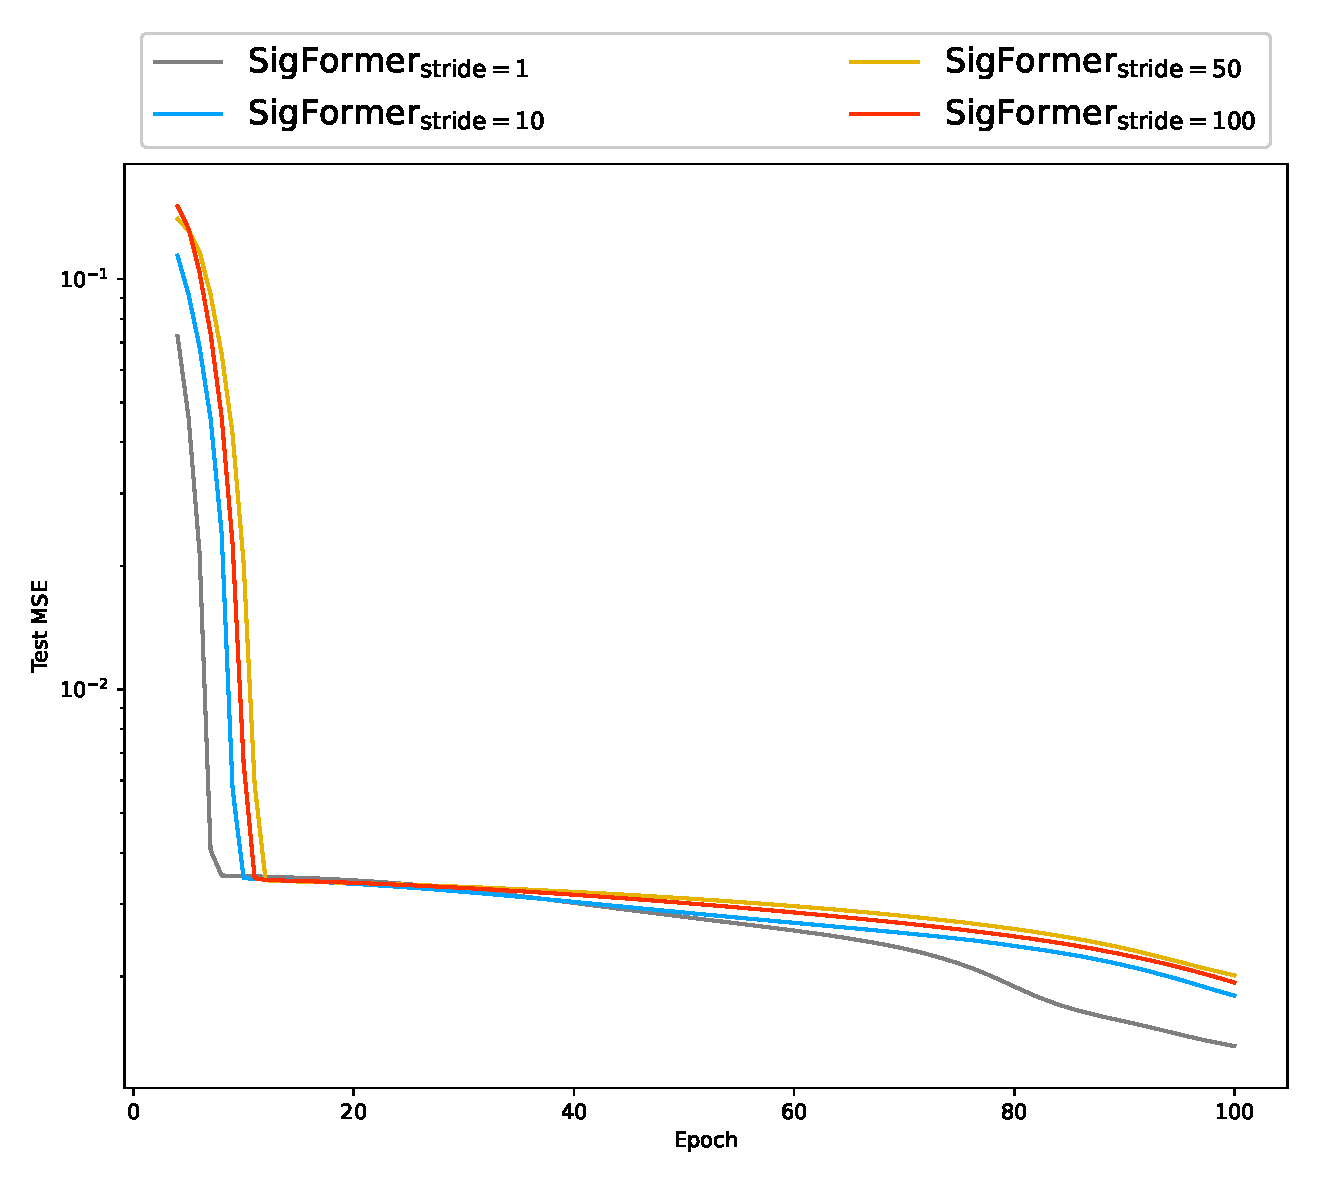
\includegraphics[width=0.32\textwidth]{fig//numerical_example1//loss_plots//rBergomi_grid=100_Hbeta_eta=1_v0=0.01.eps}
				
\includegraphics[width=0.32\textwidth]{fig//numerical_example1//loss_plots//rHeston_grid=100_Hbeta_kappa1=0.1_kappa2=0.03_theta=0.3_v0=0.01.eps}}
		}
		\caption{Loss plot for (Left:) fBms; (Middle:) rBergomi volatility processes; (Right:) rHeston volatility processes with the stride varying from $1$ to $100$. Here, the input length equals to $100$.}
	\end{figure}
	
	\subsection{Loss plots for signature-based models with the signature truncation order varying from $1$ to $5$}
	\label{subapdix-loss-plots-truncation}
	\begin{figure}[H]
		\centering
		\subfigure{
\includegraphics[width=0.30\textwidth]{fig//numerical_example2//loss_plots//fBm//fBm_grid=100_Hbeta_Trun1.eps}}
		\subfigure{
\includegraphics[width=0.30\textwidth]{fig//numerical_example2//loss_plots//fBm//fBm_grid=100_Hbeta_Trun2.eps}}
		\subfigure{
\includegraphics[width=0.30\textwidth]{fig//numerical_example2//loss_plots//fBm//fBm_grid=100_Hbeta_Trun3.eps}}
		\subfigure{
\includegraphics[width=0.30\textwidth]{fig//numerical_example2//loss_plots//fBm//fBm_grid=100_Hbeta_Trun4.eps}}
		\subfigure{
\includegraphics[width=0.30\textwidth]{fig//numerical_example2//loss_plots//fBm//fBm_grid=100_Hbeta_Trun5.eps}}
		\caption{Loss plot for fBms with signature truncation order ranging from (left to right and top to bottom:) $\{1,\,2,\,3,\,4,\,5\}$. Here $H\sim\text{Beta}(1,\,9)$ and the input lengths equal to $100$. }
	\end{figure}
	
	\begin{figure}[H]
		\centering
		\subfigure{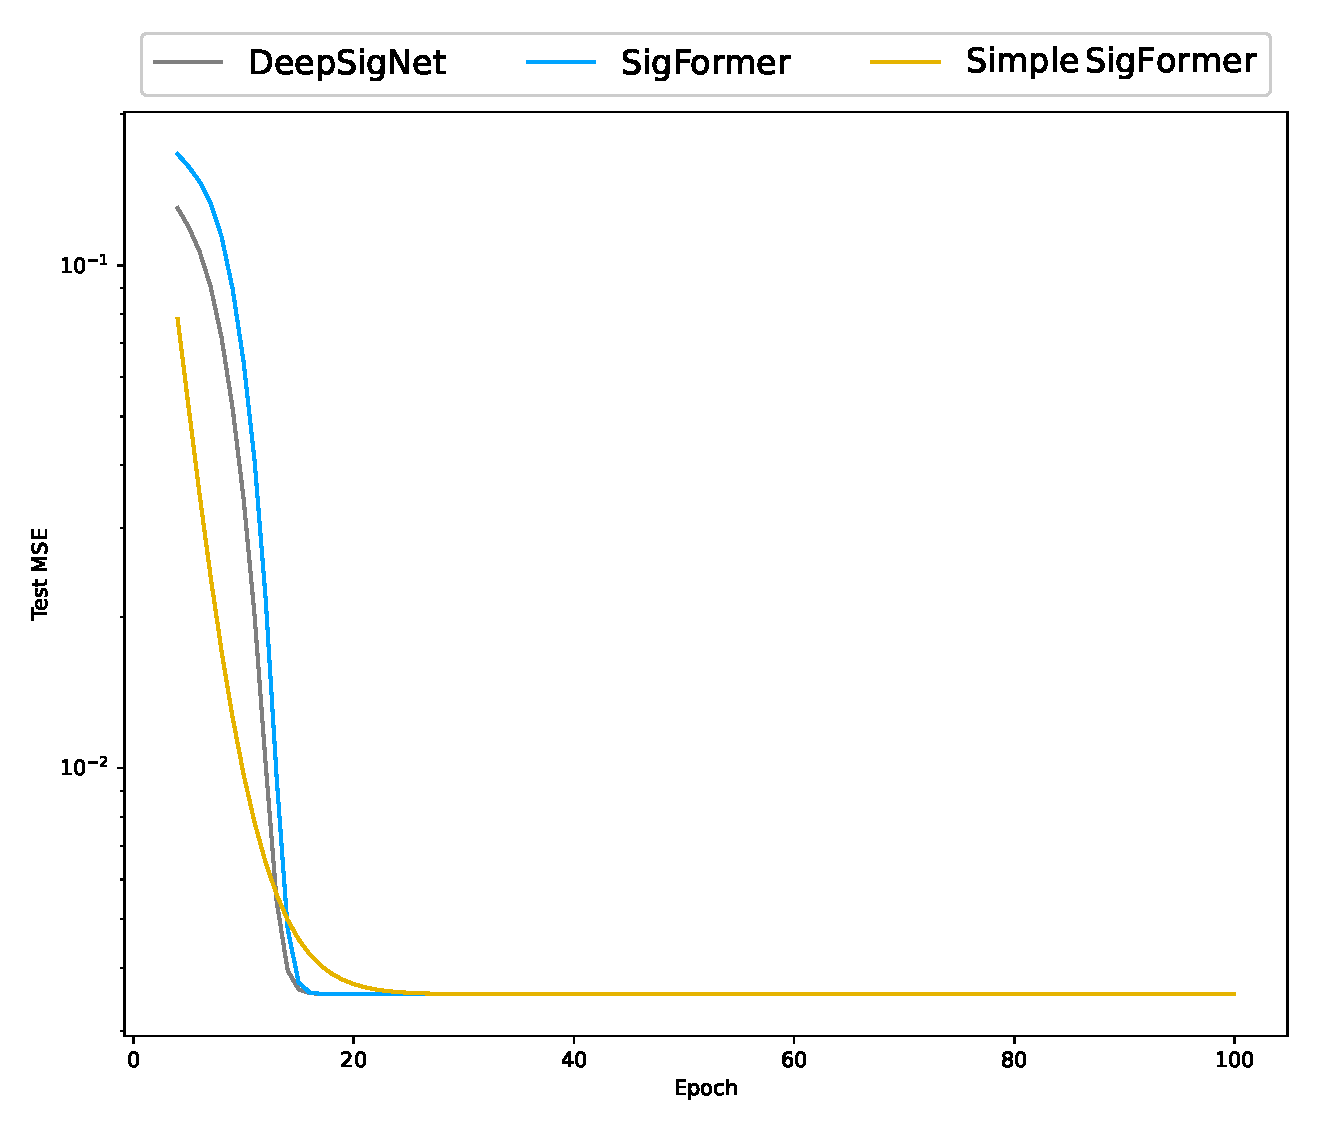
\includegraphics[width=0.30\textwidth]{fig//numerical_example2//loss_plots//rBergomi//rBergomi_grid=100_Hbeta_eta=1_v0=0.01_Trun1.eps}}
		\subfigure{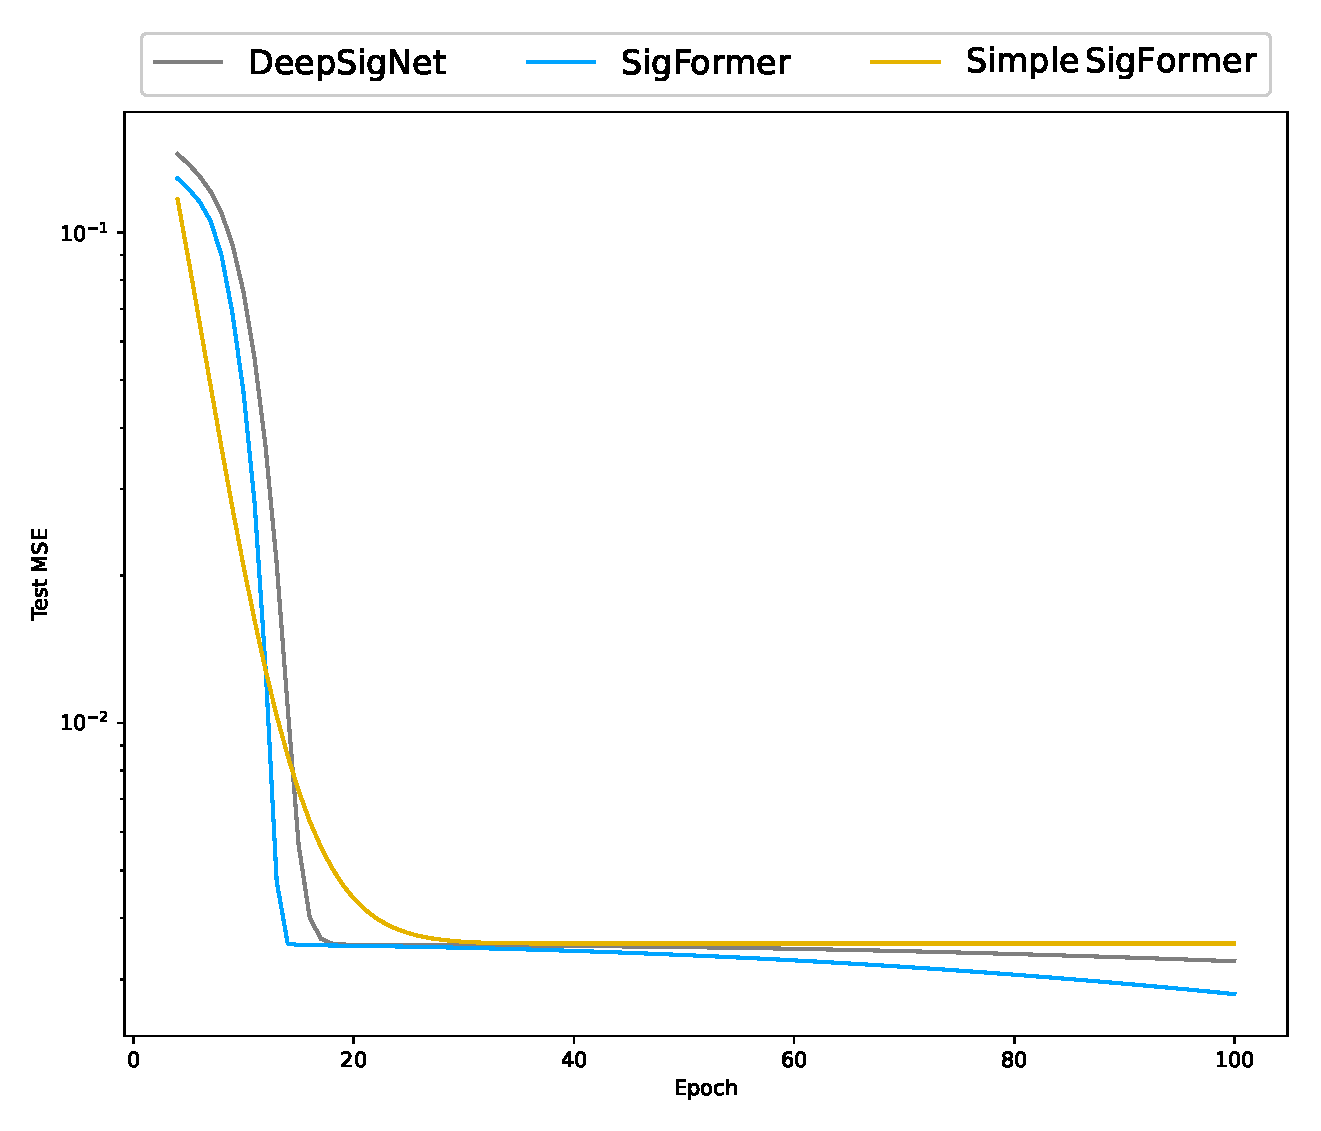
\includegraphics[width=0.30\textwidth]{fig//numerical_example2//loss_plots//rBergomi//rBergomi_grid=100_Hbeta_eta=1_v0=0.01_Trun2.eps}}
		\subfigure{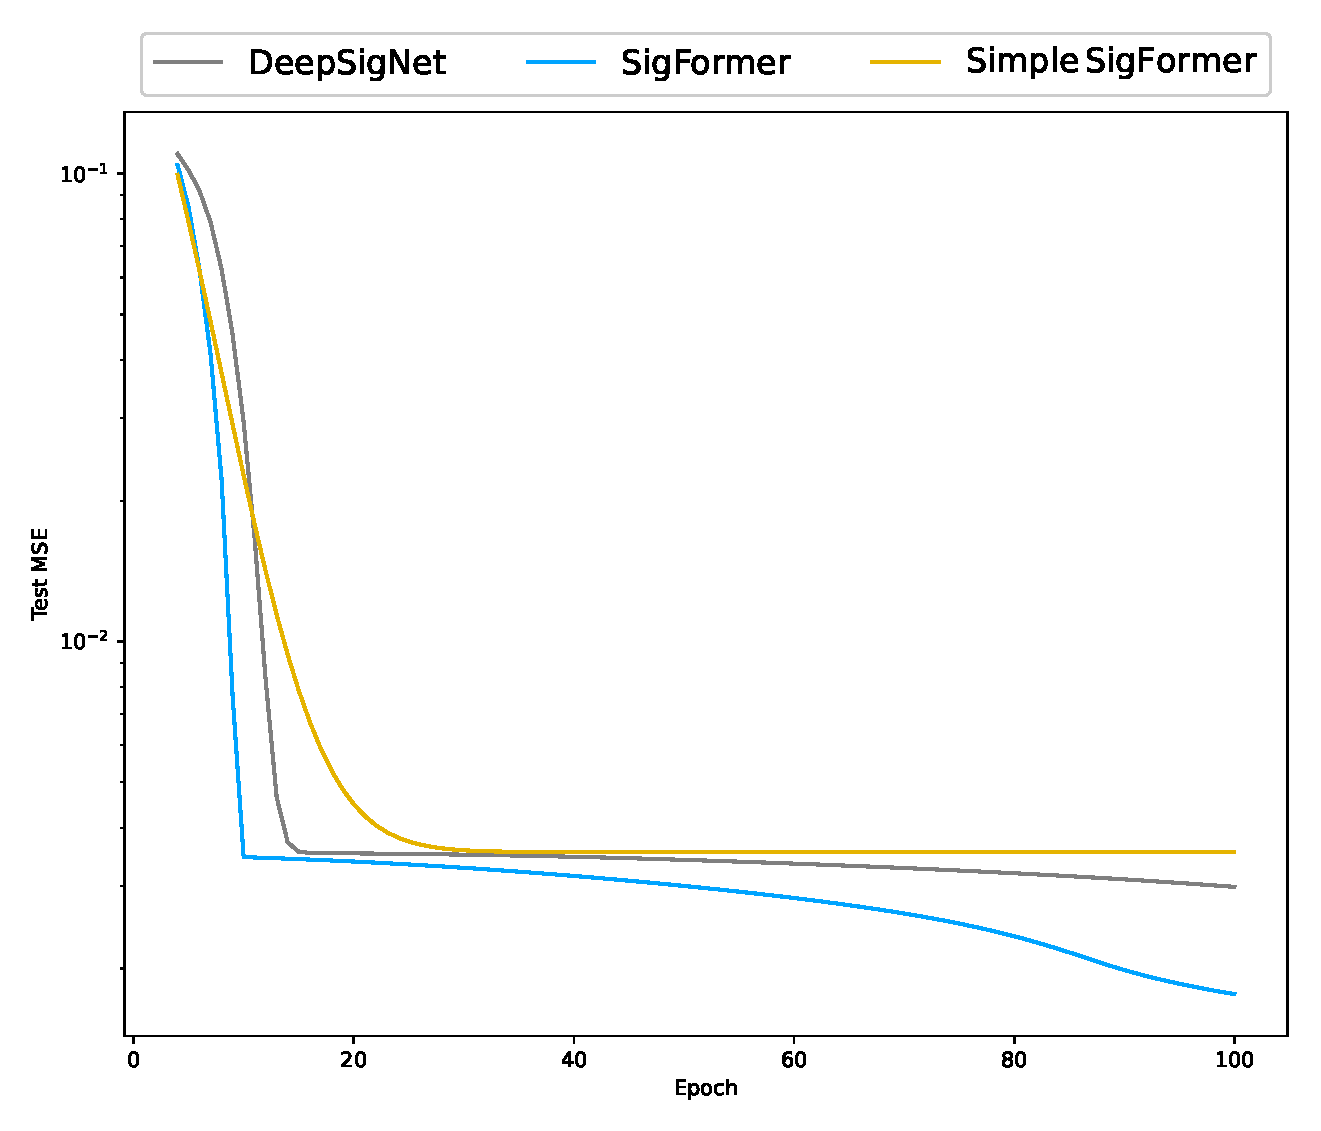
\includegraphics[width=0.30\textwidth]{fig//numerical_example2//loss_plots//rBergomi//rBergomi_grid=100_Hbeta_eta=1_v0=0.01_Trun3.eps}}
		\subfigure{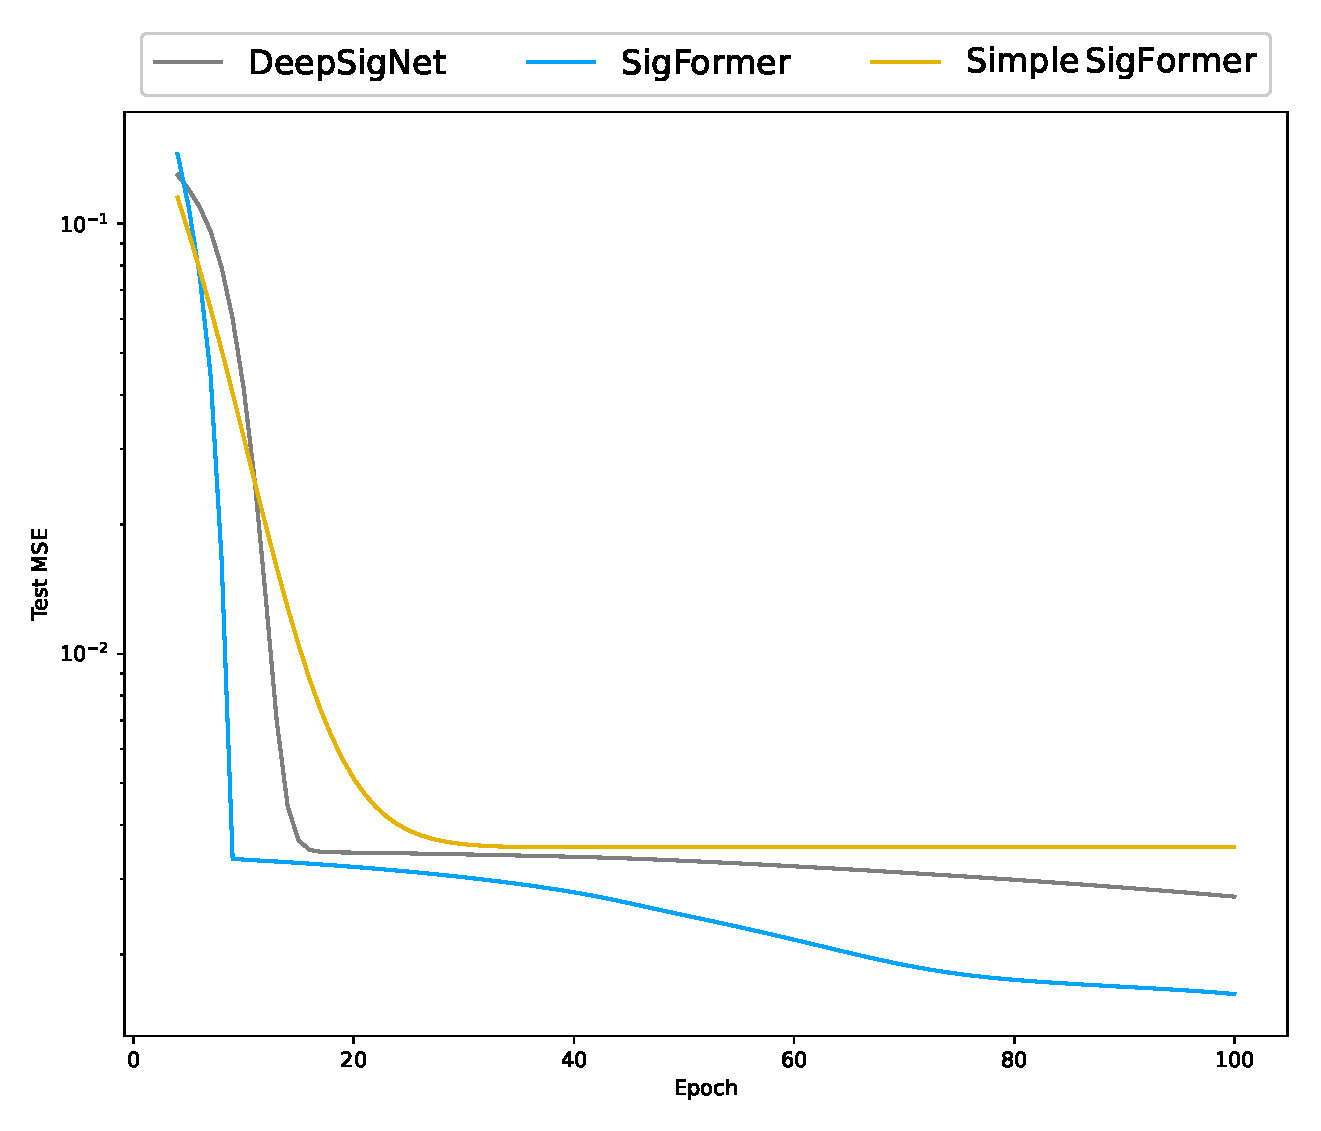
\includegraphics[width=0.30\textwidth]{fig//numerical_example2//loss_plots//rBergomi//rBergomi_grid=100_Hbeta_eta=1_v0=0.01_Trun4.eps}}
		\subfigure{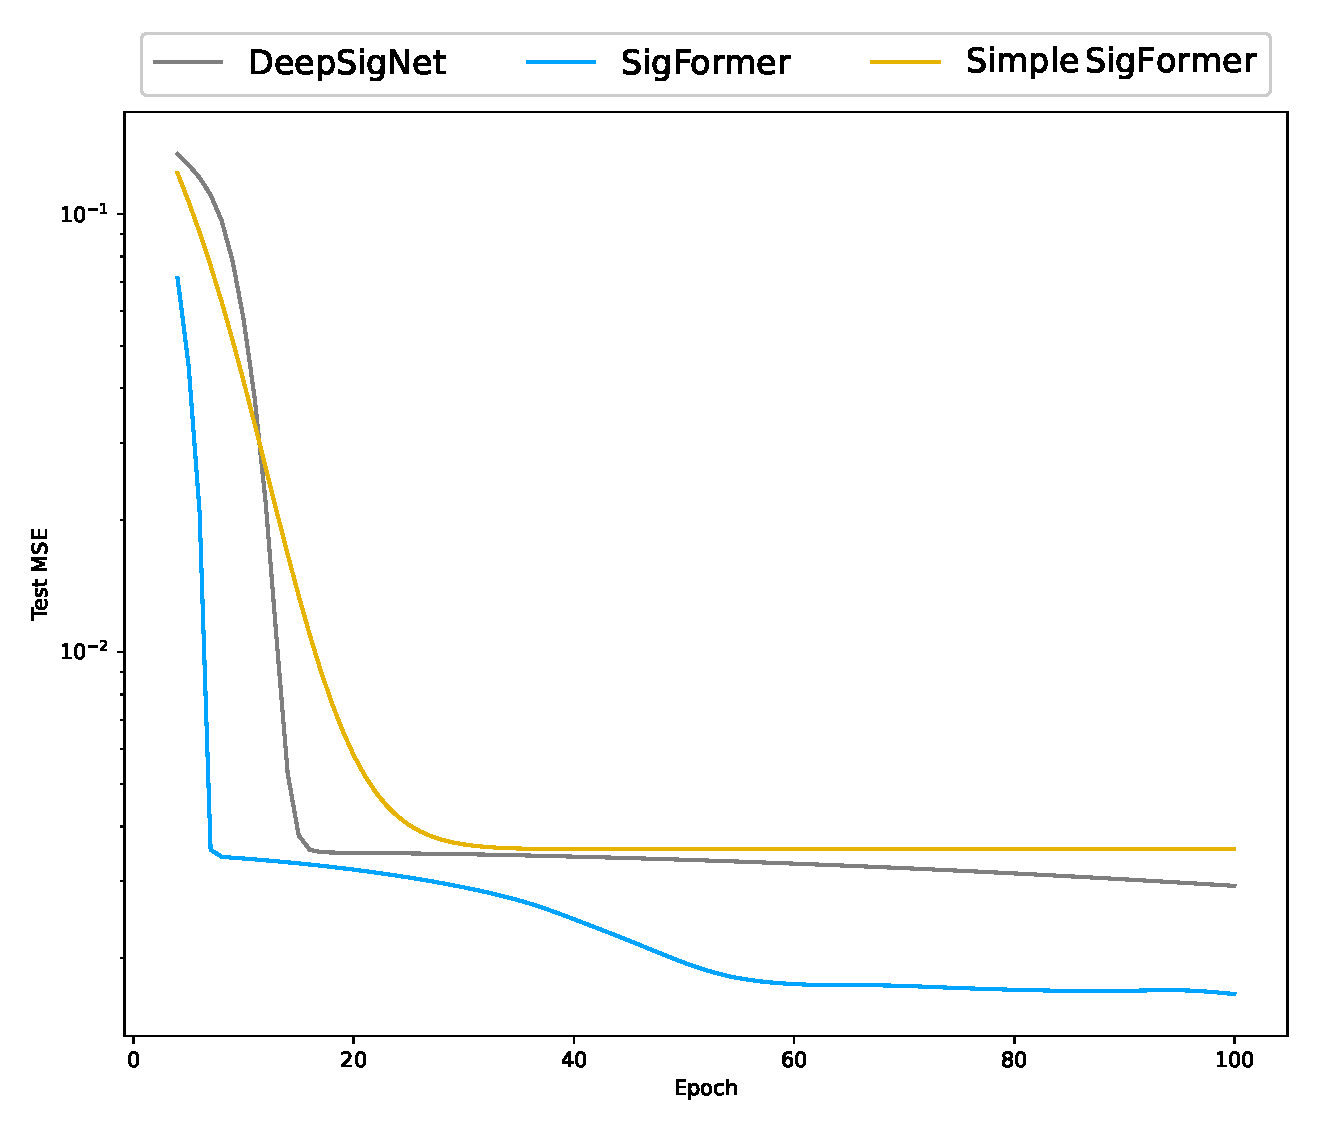
\includegraphics[width=0.30\textwidth]{fig//numerical_example2//loss_plots//rBergomi//rBergomi_grid=100_Hbeta_eta=1_v0=0.01_Trun5.eps}}
		\caption{Loss plot for rBergomi volatility processes with signature truncation order ranging from (left to right and top to bottom:) $\{1,\,2,\,3,\,4,\,5\}$. Here $H\sim\text{Beta}(1,\,9)$ and the input lengths equal to $100$. }
	\end{figure}
	
	\begin{figure}[H]
		\centering
		\subfigure{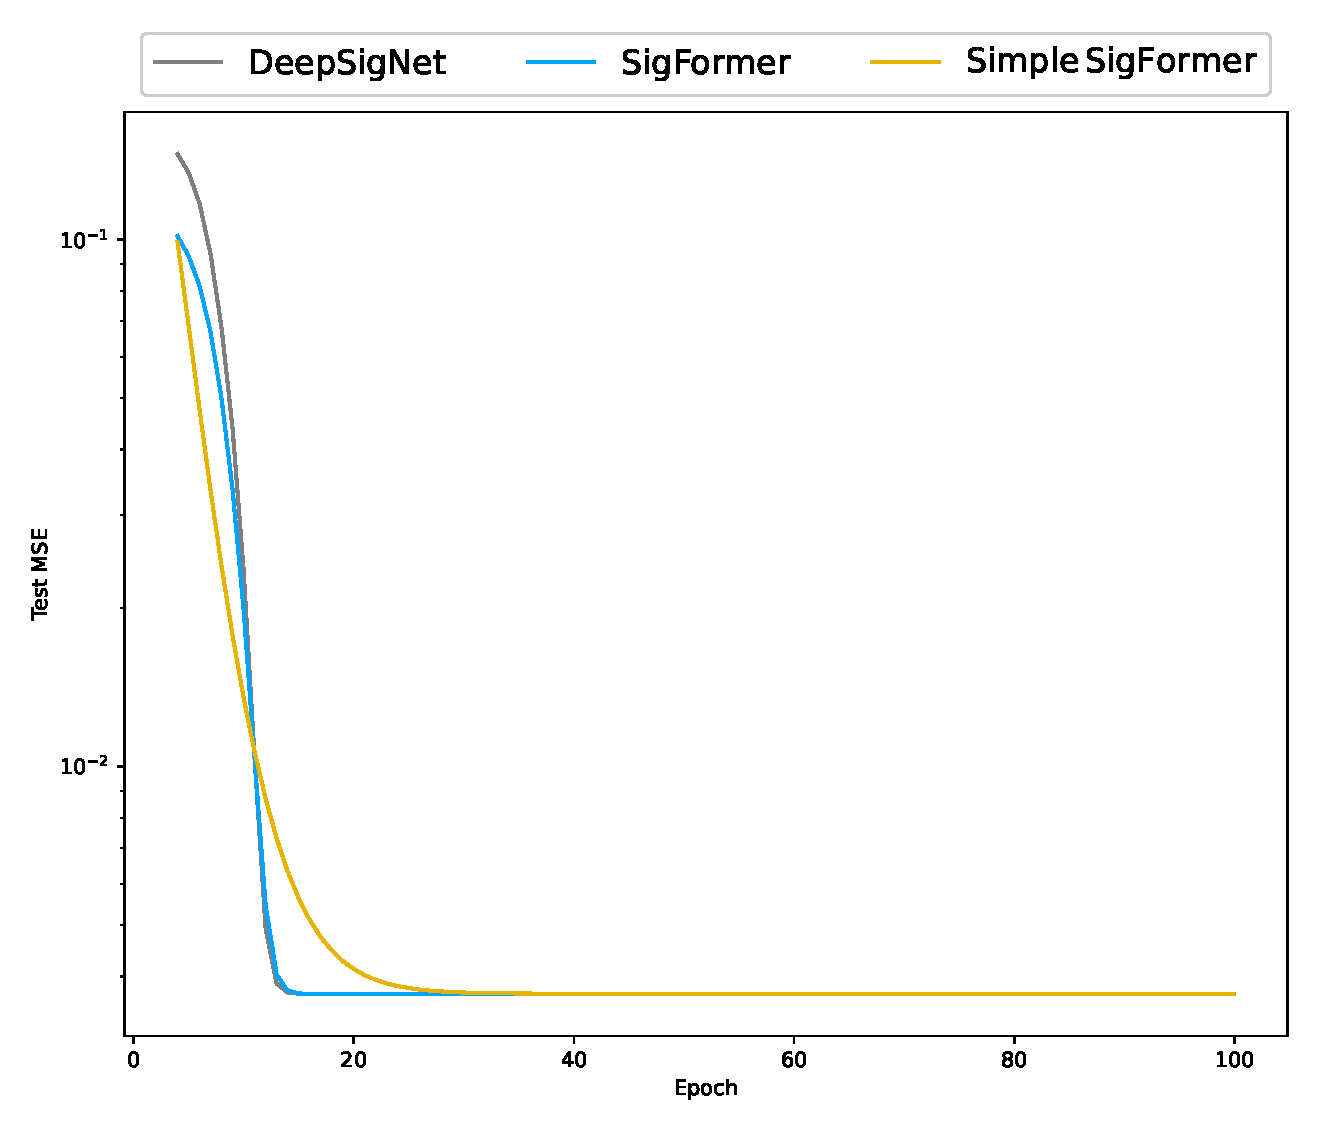
\includegraphics[width=0.30\textwidth]{fig//numerical_example2//loss_plots//rHeston//rHeston_grid=100_Hbeta_kappa1=0.1_kappa2=0.03_theta=0.3_v0=0.01_Trun1.eps}}
		\subfigure{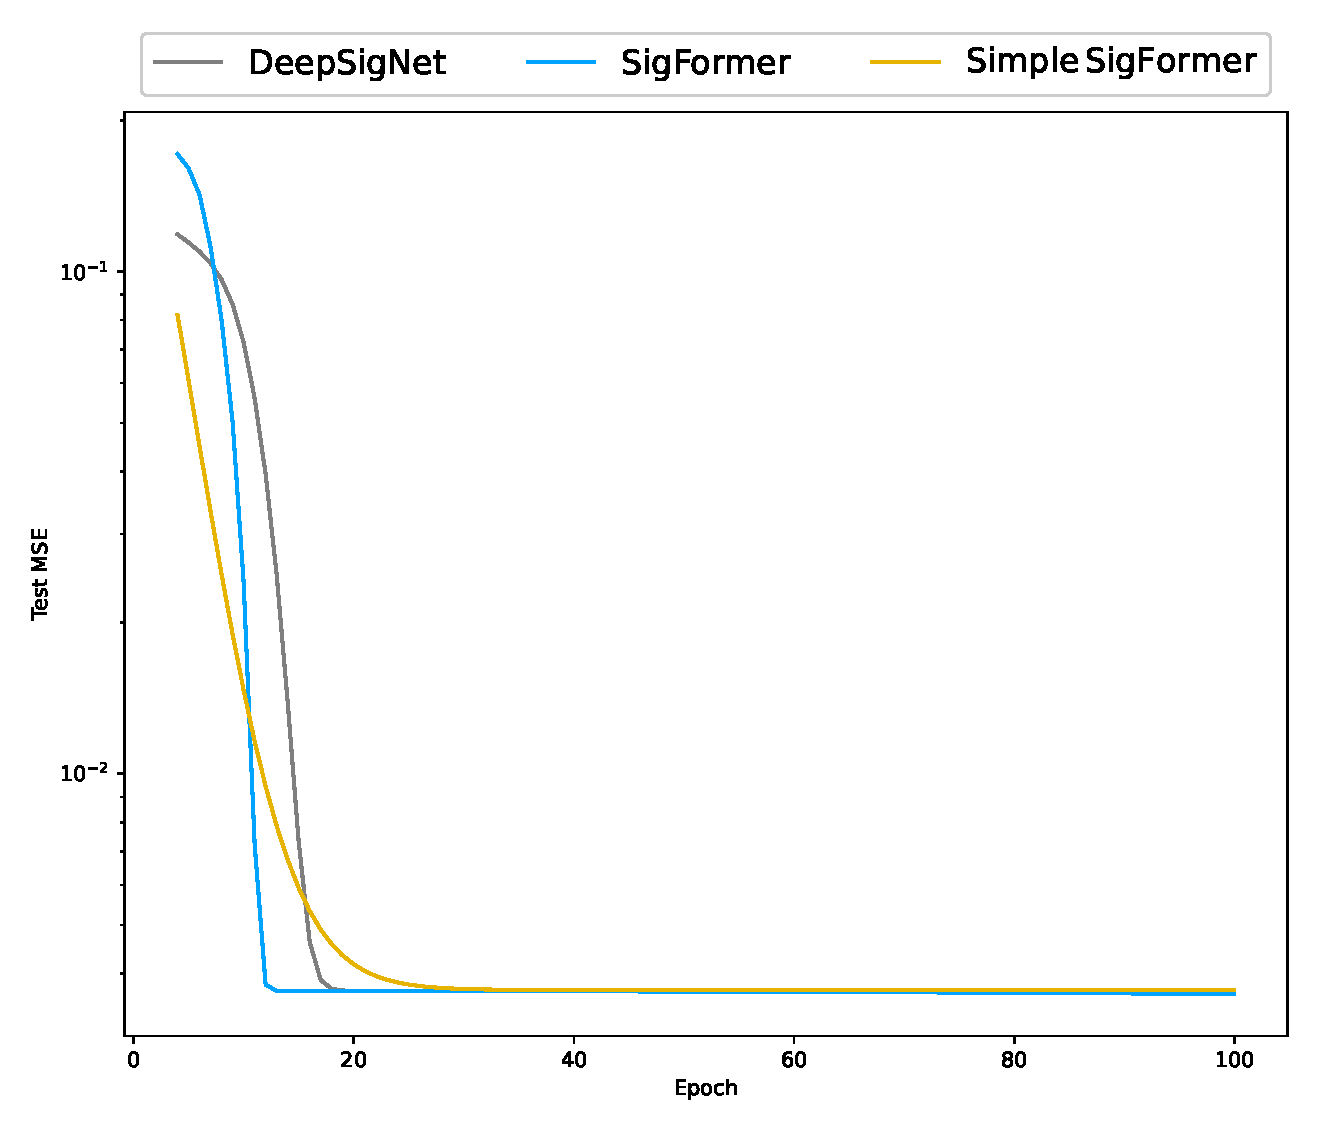
\includegraphics[width=0.30\textwidth]{fig//numerical_example2//loss_plots//rHeston//rHeston_grid=100_Hbeta_kappa1=0.1_kappa2=0.03_theta=0.3_v0=0.01_Trun2.eps}}
		\subfigure{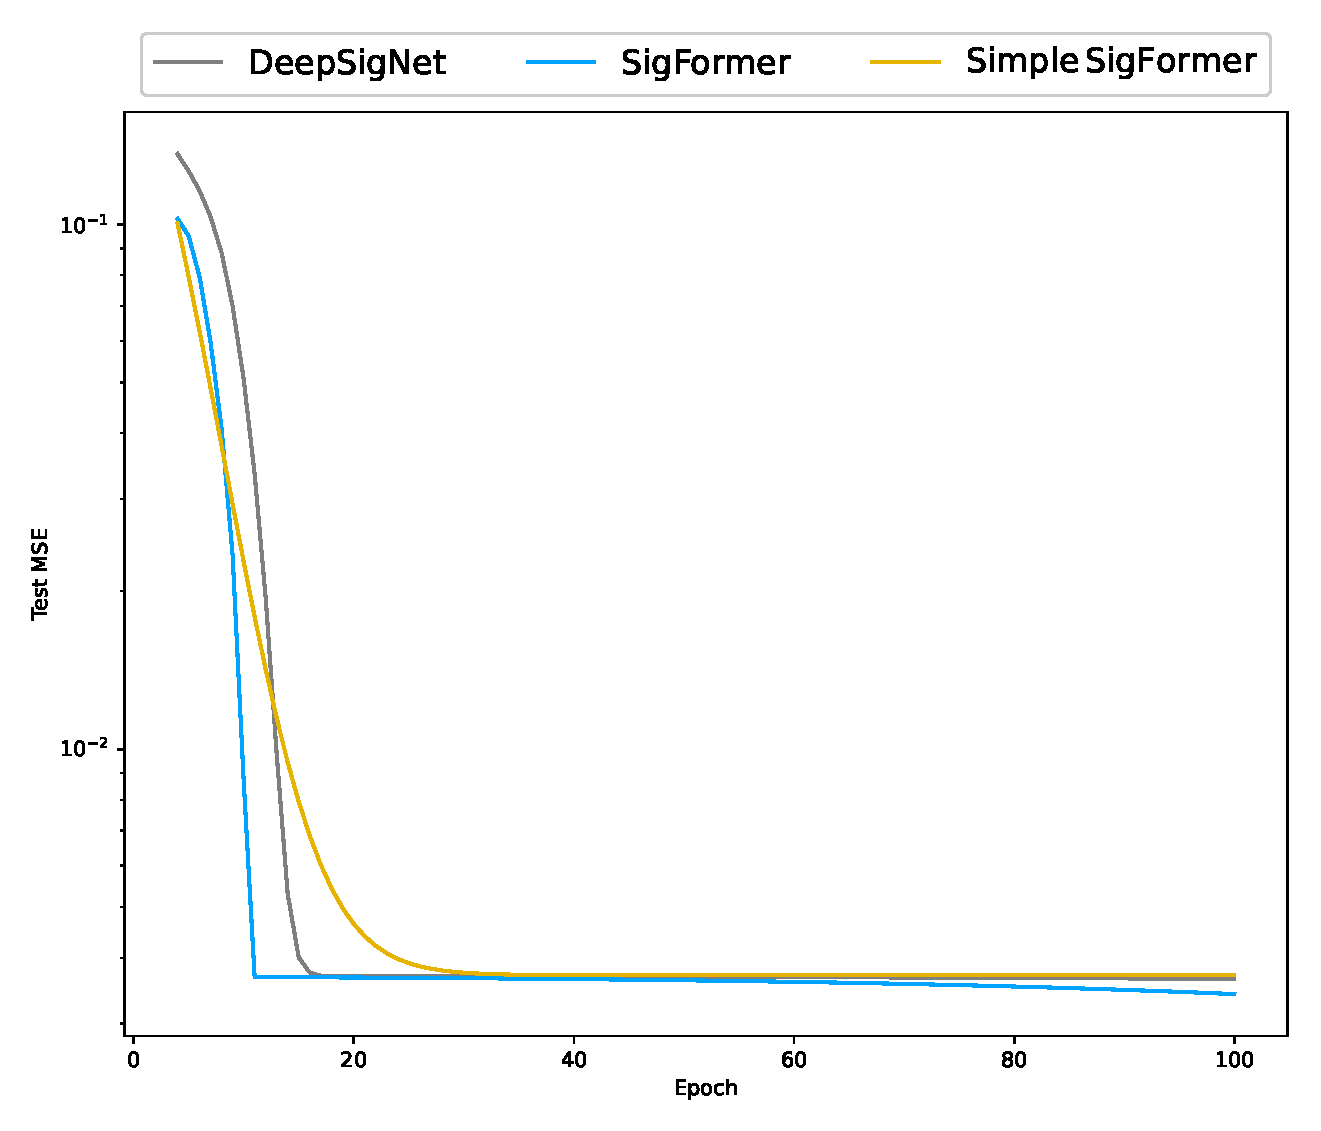
\includegraphics[width=0.30\textwidth]{fig//numerical_example2//loss_plots//rHeston//rHeston_grid=100_Hbeta_kappa1=0.1_kappa2=0.03_theta=0.3_v0=0.01_Trun3.eps}}
		\subfigure{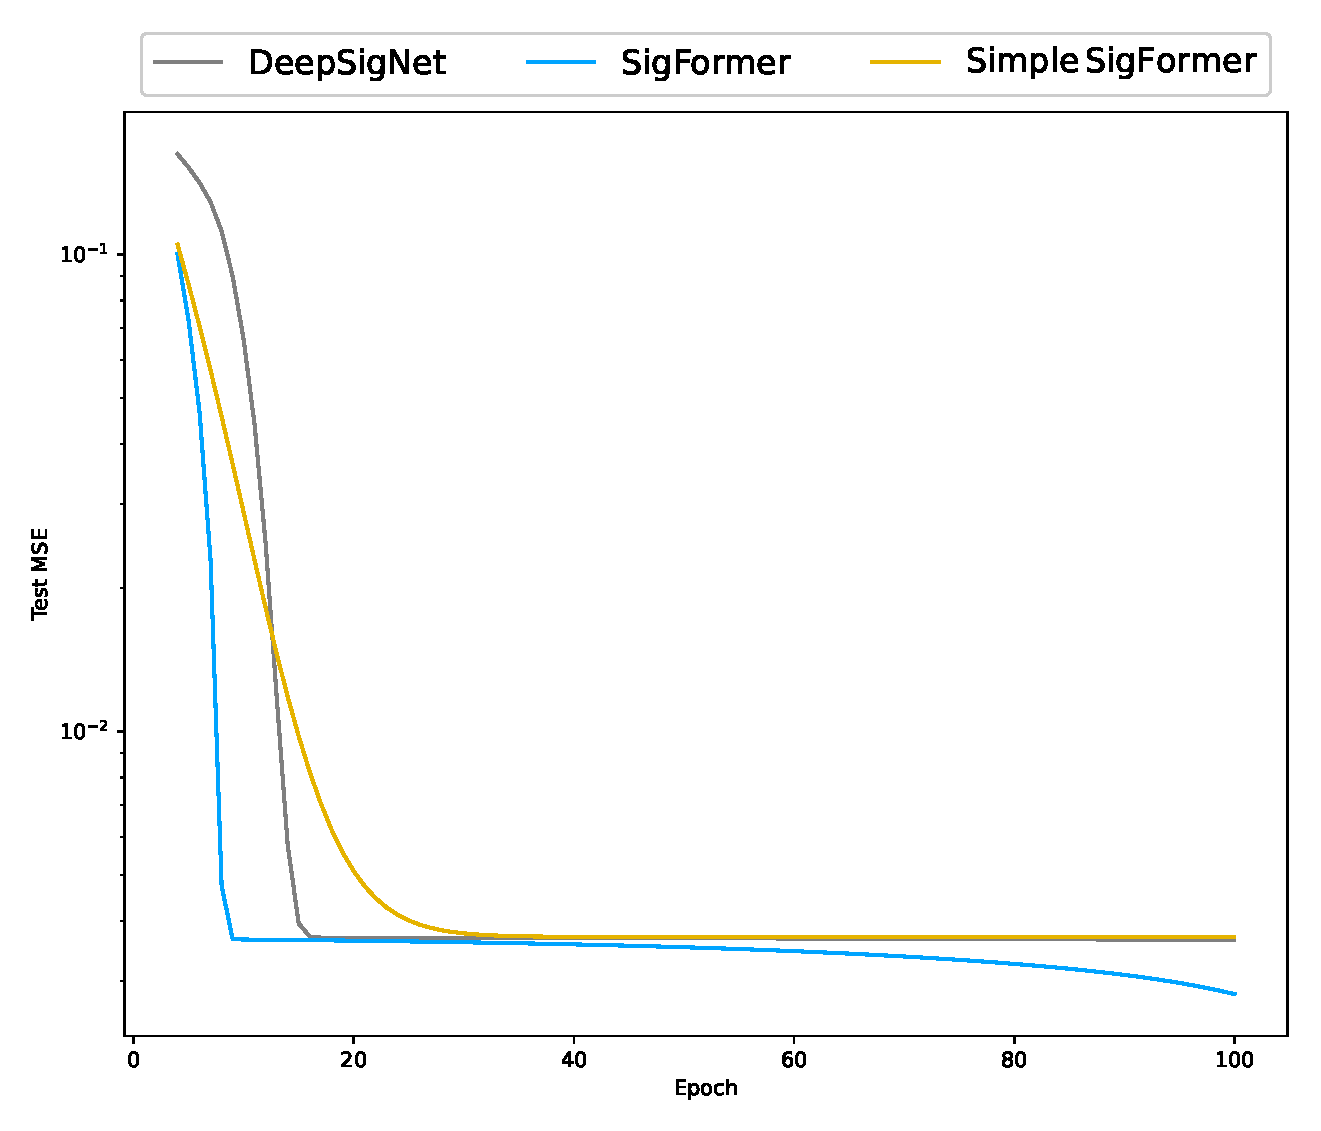
\includegraphics[width=0.30\textwidth]{fig//numerical_example2//loss_plots//rHeston//rHeston_grid=100_Hbeta_kappa1=0.1_kappa2=0.03_theta=0.3_v0=0.01_Trun4.eps}}
		\subfigure{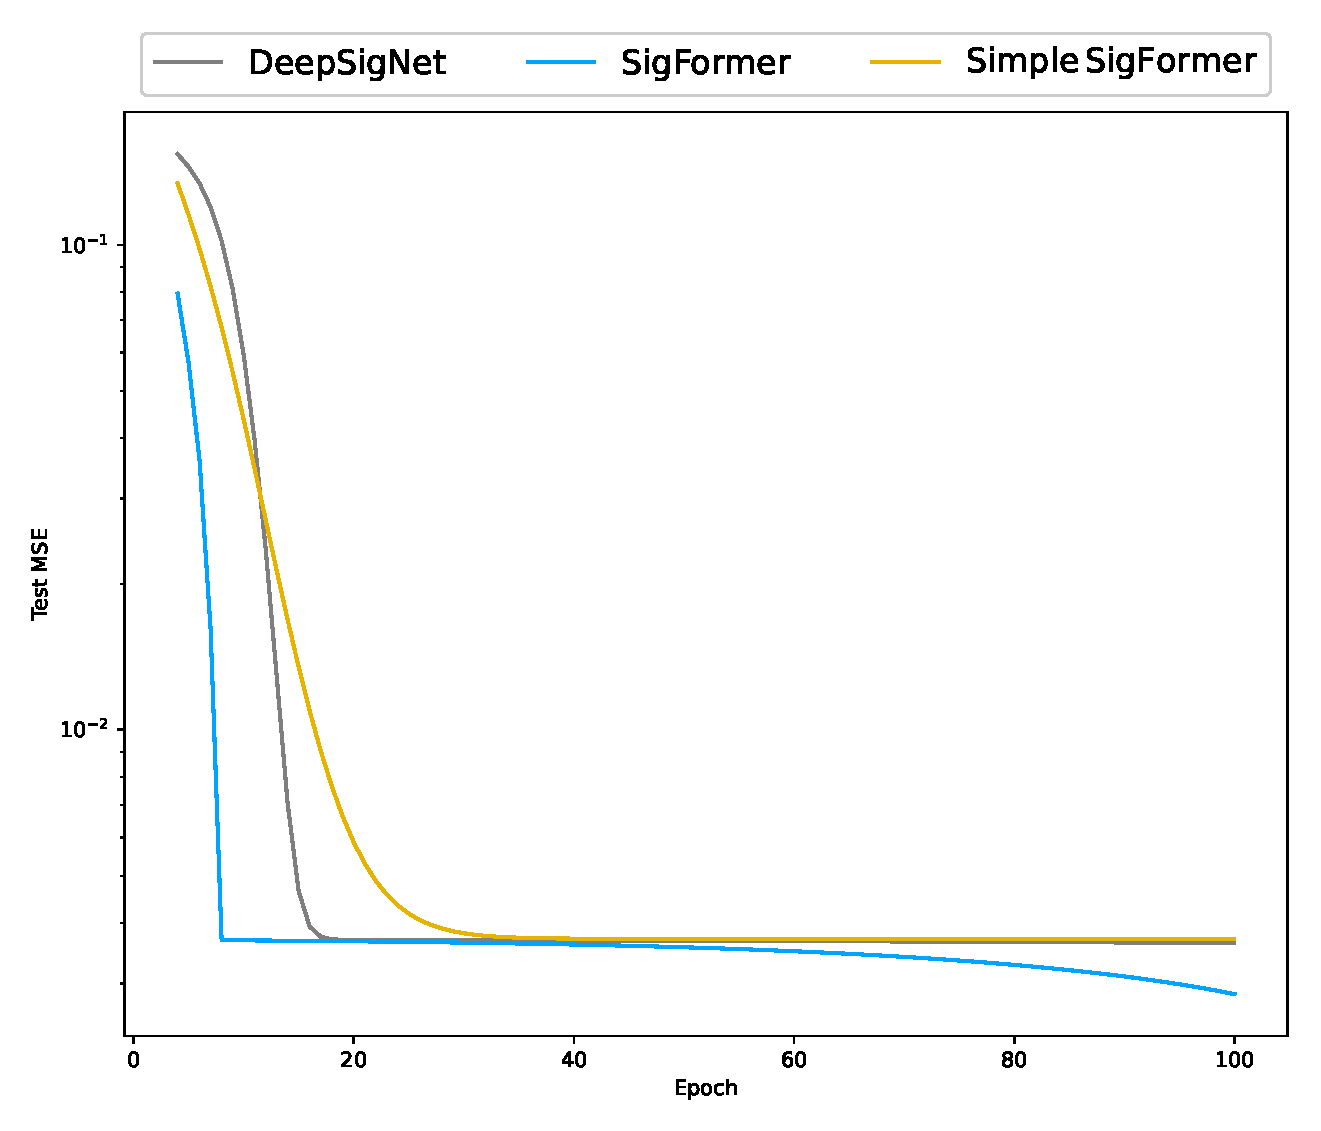
\includegraphics[width=0.30\textwidth]{fig//numerical_example2//loss_plots//rHeston//rHeston_grid=100_Hbeta_kappa1=0.1_kappa2=0.03_theta=0.3_v0=0.01_Trun5.eps}}
		\caption{Loss plot for rHeston volatility processes with signature truncation order ranging from (left to right and top to bottom:) $\{1,\,2,\,3,\,4,\,5\}$. Here $H\sim\text{Beta}(1,\,9)$ and the input lengths equal to $100$. }
	\end{figure}
	
	\subsection{Loss plots for different SigFormer models with input lengths varying from $100$ to $300$}
	\label{subapdix-loss-plots-structure}
	\begin{figure}[H]
	\centering
	\resizebox{0.9\textwidth}{!}{
		\subfigure[The input length equals to $100$.]{
			
\includegraphics[width=0.32\textwidth]{fig//numerical_example3//loss_plots//uniform//fBm_grid=100_Huniform.eps}
			
\includegraphics[width=0.32\textwidth]{fig//numerical_example3//loss_plots//uniform//rBergomi_grid=100_Huniform_eta=1_v0=0.01.eps}
			
\includegraphics[width=0.32\textwidth]{fig//numerical_example3//loss_plots//uniform//rHeston_grid=100_Huniform_kappa1=0.1_kappa2=0.03_theta=0.3_v0=0.01.eps}}
	}
	\resizebox{0.9\textwidth}{!}{
		\subfigure[The input length equals to $200$.]{
			
\includegraphics[width=0.32\textwidth]{fig//numerical_example3//loss_plots//uniform//fBm_grid=200_Huniform.eps}
			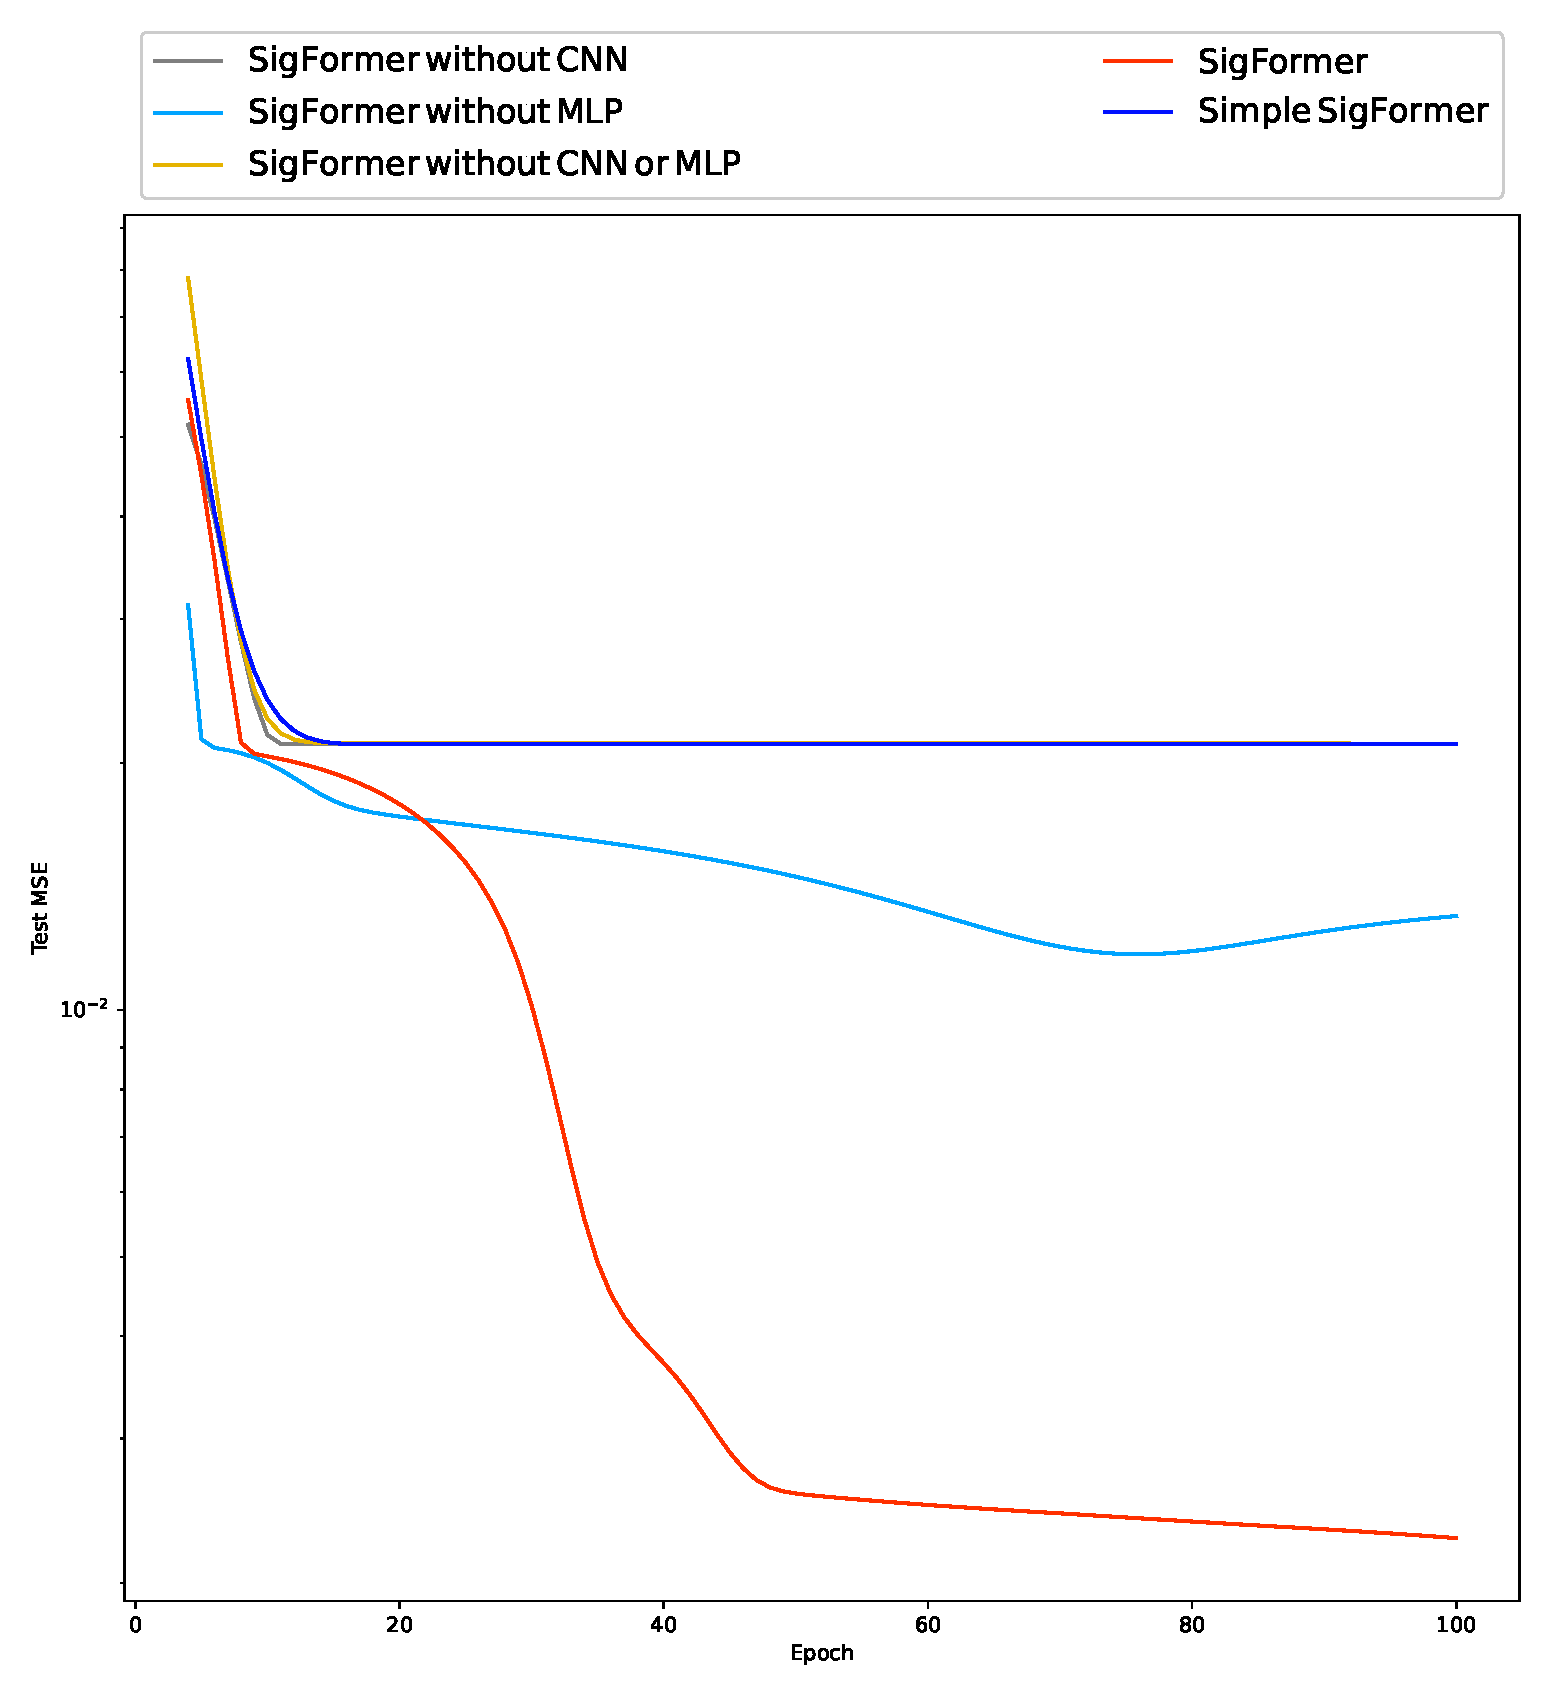
\includegraphics[width=0.32\textwidth]{fig//numerical_example3//loss_plots//uniform//rBergomi_grid=200_Huniform_eta=1_v0=0.01.eps}
			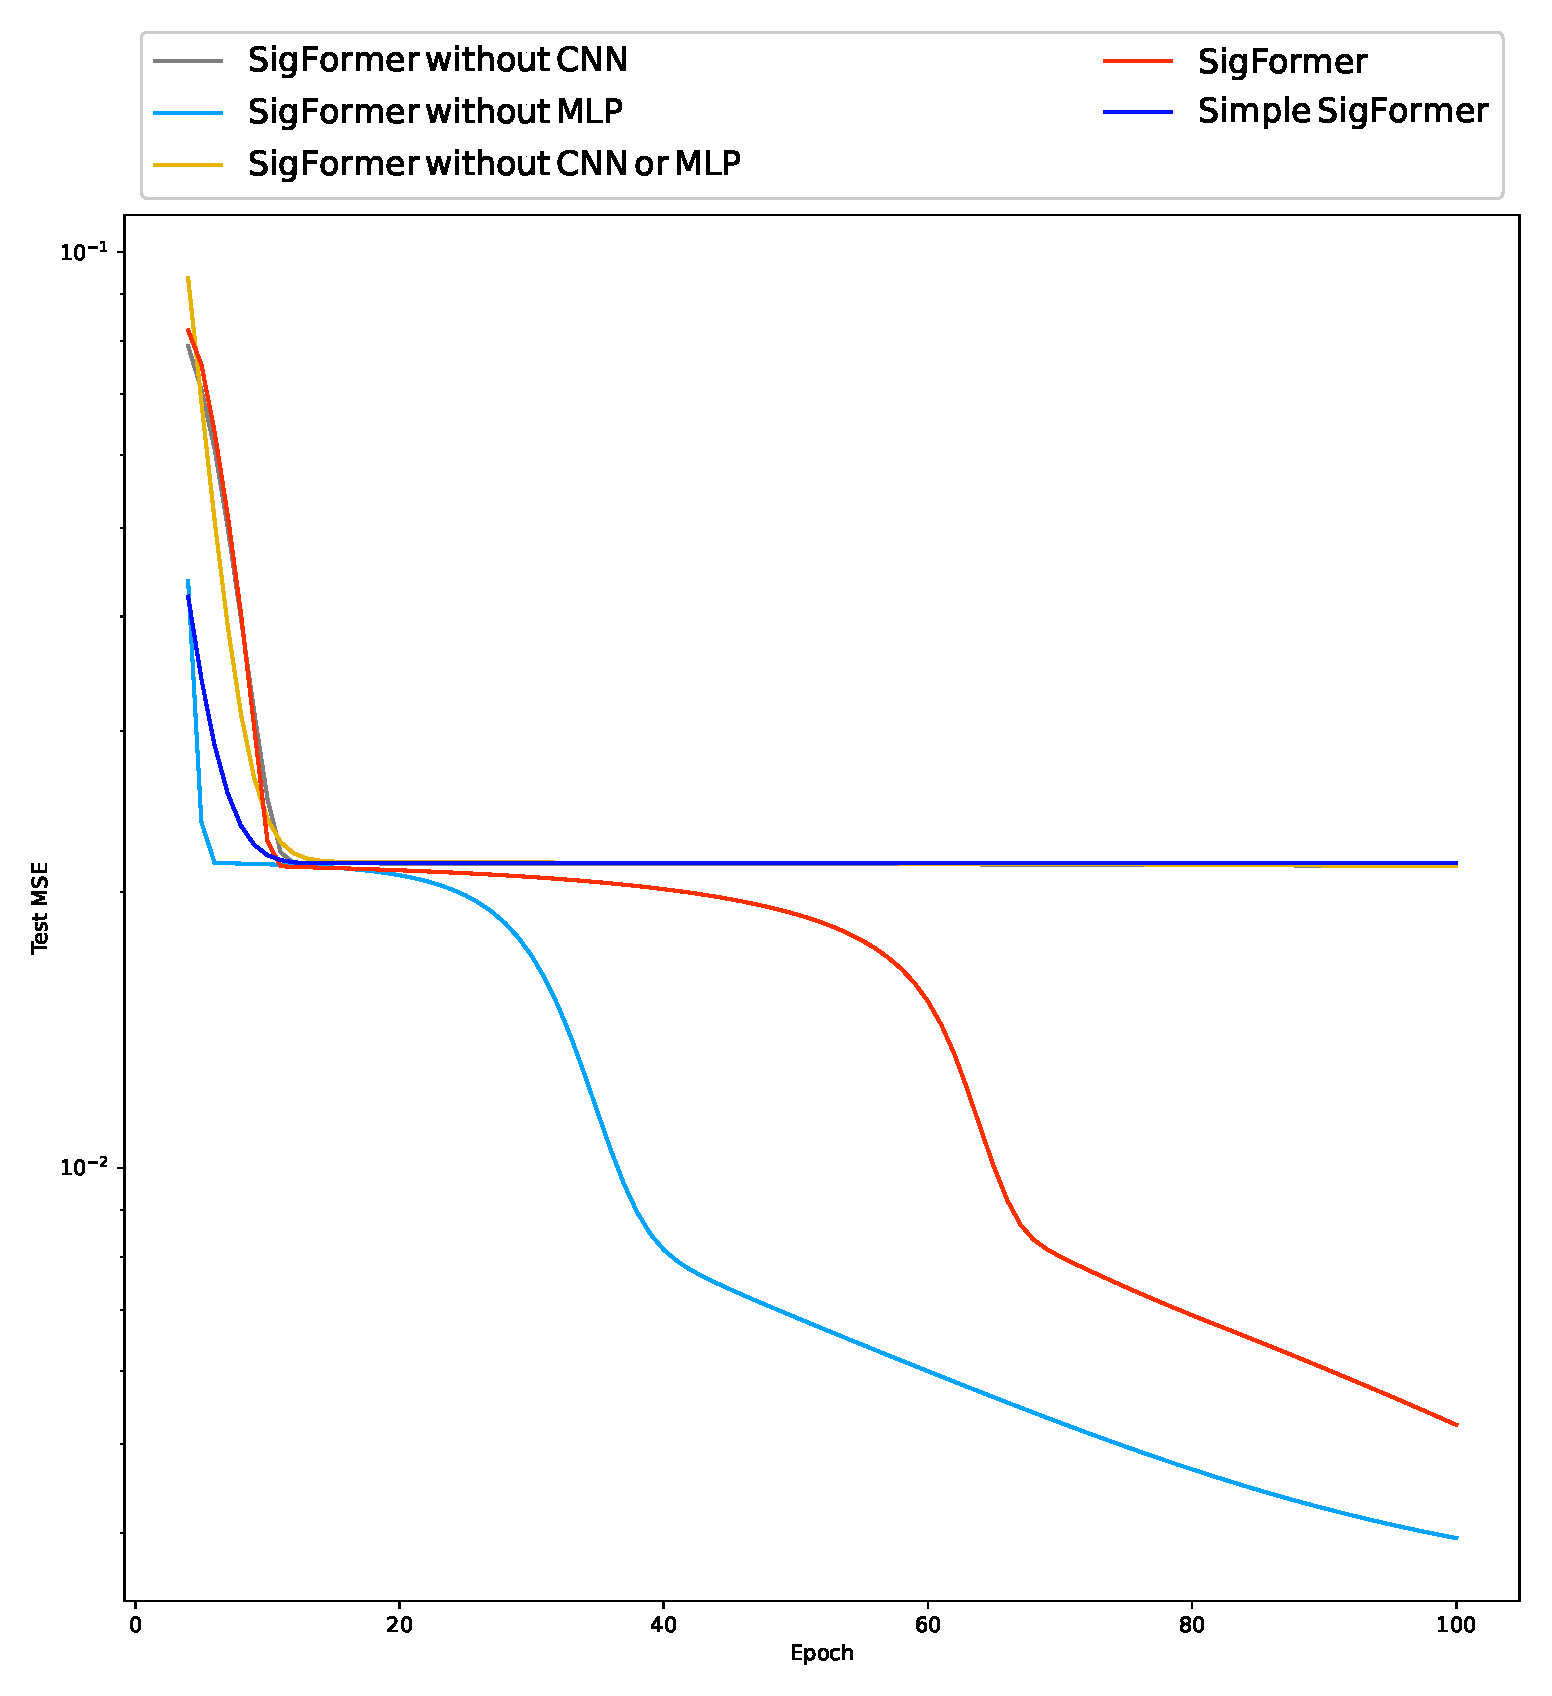
\includegraphics[width=0.32\textwidth]{fig//numerical_example3//loss_plots//uniform//rHeston_grid=200_Huniform_kappa1=0.1_kappa2=0.03_theta=0.3_v0=0.01.eps}}
	}
	\resizebox{0.9\textwidth}{!}{
		\subfigure[The input length equals to $300$.]{
			
\includegraphics[width=0.32\textwidth]{fig//numerical_example3//loss_plots//uniform//fBm_grid=300_Huniform.eps}
			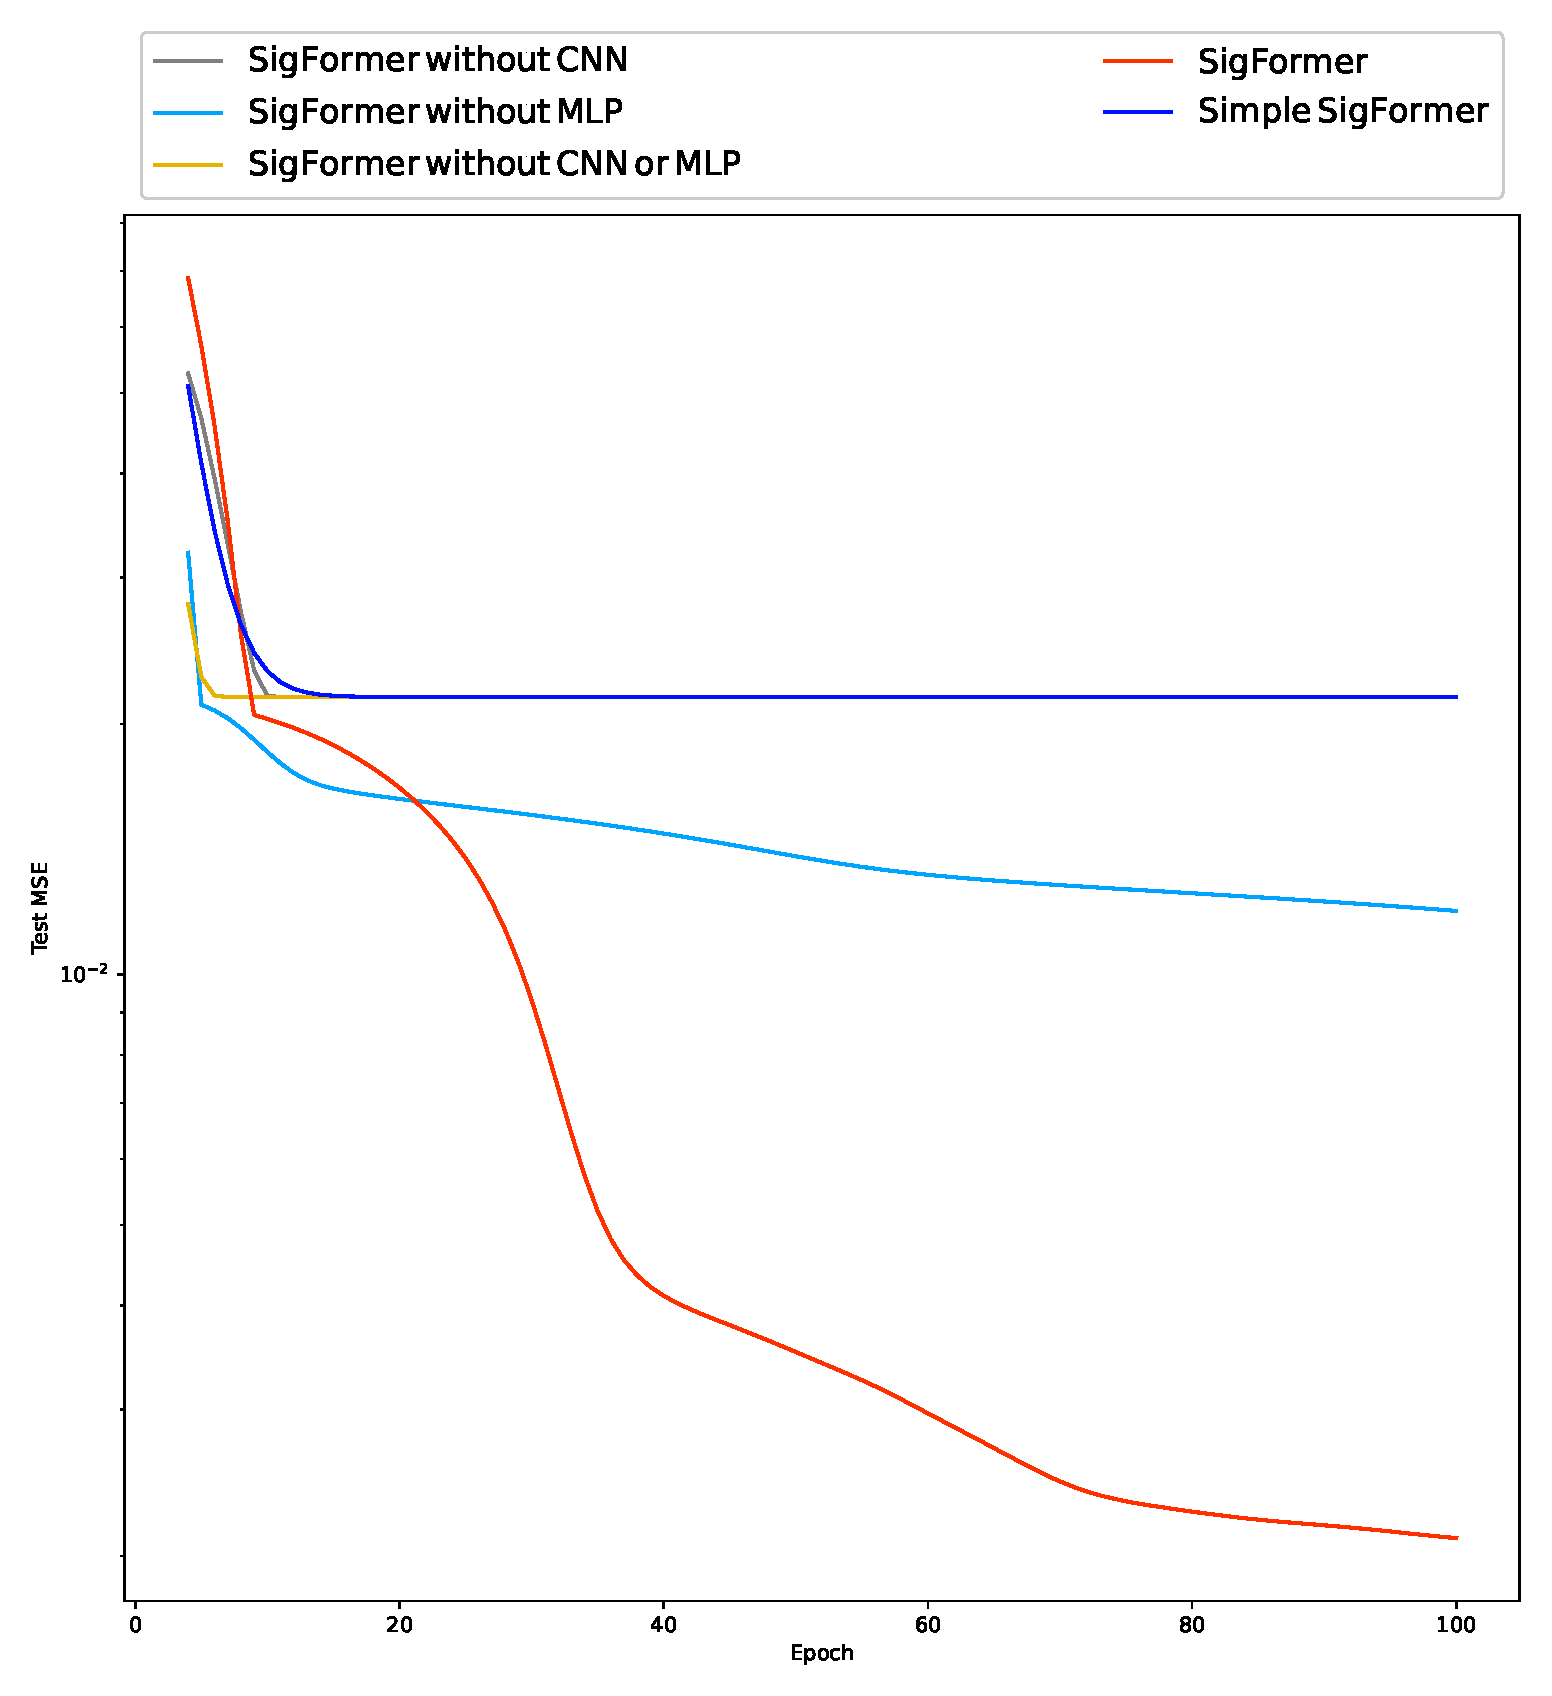
\includegraphics[width=0.32\textwidth]{fig//numerical_example3//loss_plots//uniform//rBergomi_grid=300_Huniform_eta=1_v0=0.01.eps}
			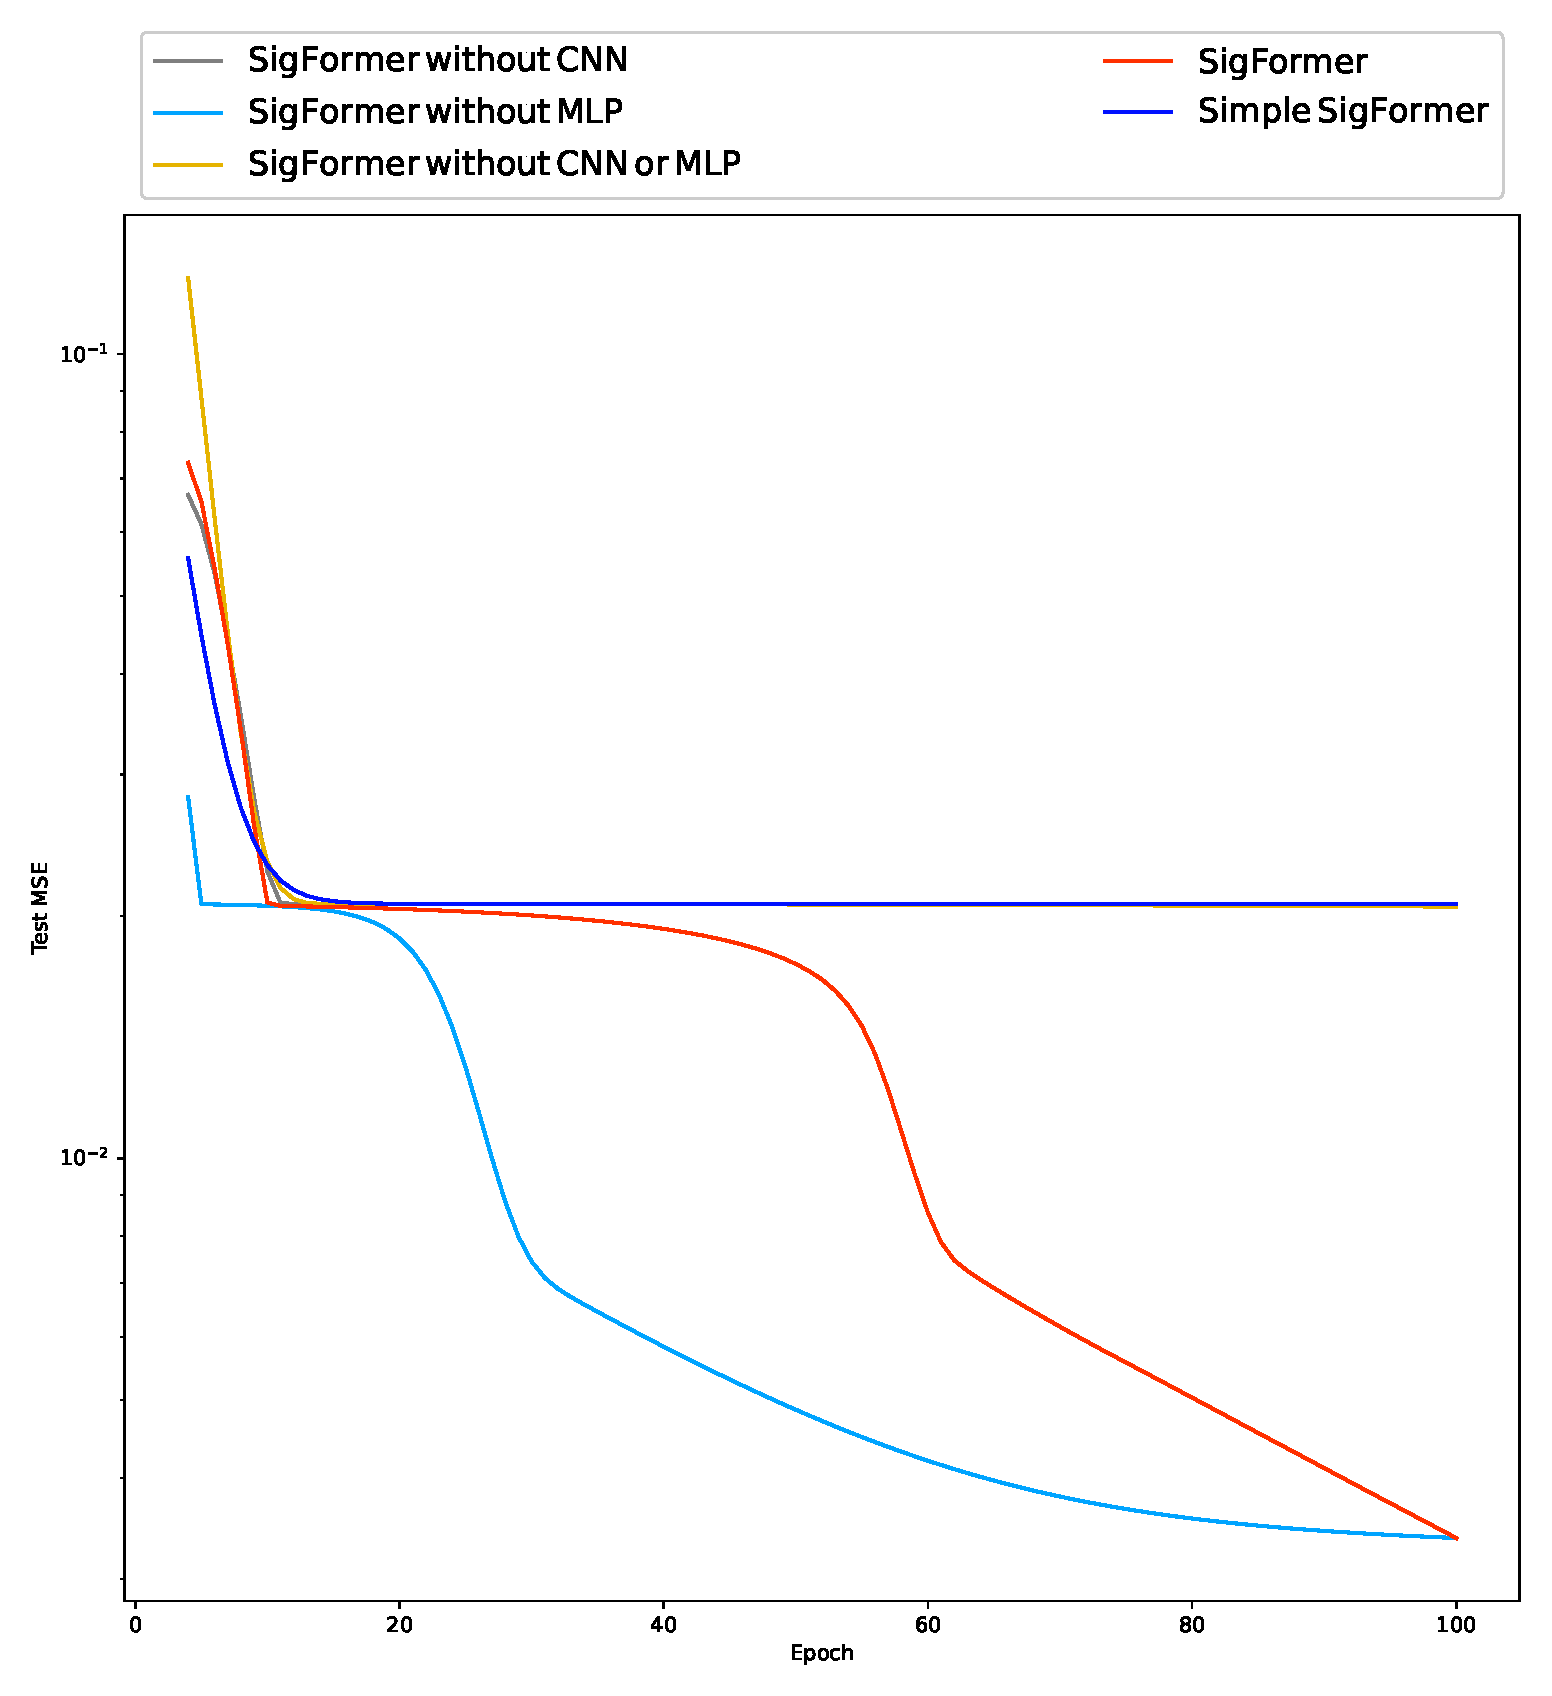
\includegraphics[width=0.32\textwidth]{fig//numerical_example3//loss_plots//uniform//rHeston_grid=300_Huniform_kappa1=0.1_kappa2=0.03_theta=0.3_v0=0.01.eps}}
	}
	\caption{Loss plot for (Left:) fBms; (Middle:) rBergomi volatility processes; (Right:) rHeston volatility processes with input lengths varying from $100$ to $300$ and $H\sim\text{Uniform}(0,0.5)$. }
	\end{figure}
	
	\begin{figure}[H]
	\centering
	\resizebox{0.9\textwidth}{!}{
		\subfigure[The input length equals to $100$.]{
			
\includegraphics[width=0.32\textwidth]{fig//numerical_example3//loss_plots//beta//fBm_grid=100_Hbeta.eps}
			
\includegraphics[width=0.32\textwidth]{fig//numerical_example3//loss_plots//beta//rBergomi_grid=100_Hbeta_eta=1_v0=0.01.eps}
			
\includegraphics[width=0.32\textwidth]{fig//numerical_example3//loss_plots//beta//rHeston_grid=100_Hbeta_kappa1=0.1_kappa2=0.03_theta=0.3_v0=0.01.eps}}
	}
	\resizebox{0.9\textwidth}{!}{
		\subfigure[The input length equals to $200$.]{
			
\includegraphics[width=0.32\textwidth]{fig//numerical_example3//loss_plots//beta//fBm_grid=200_Hbeta.eps}
			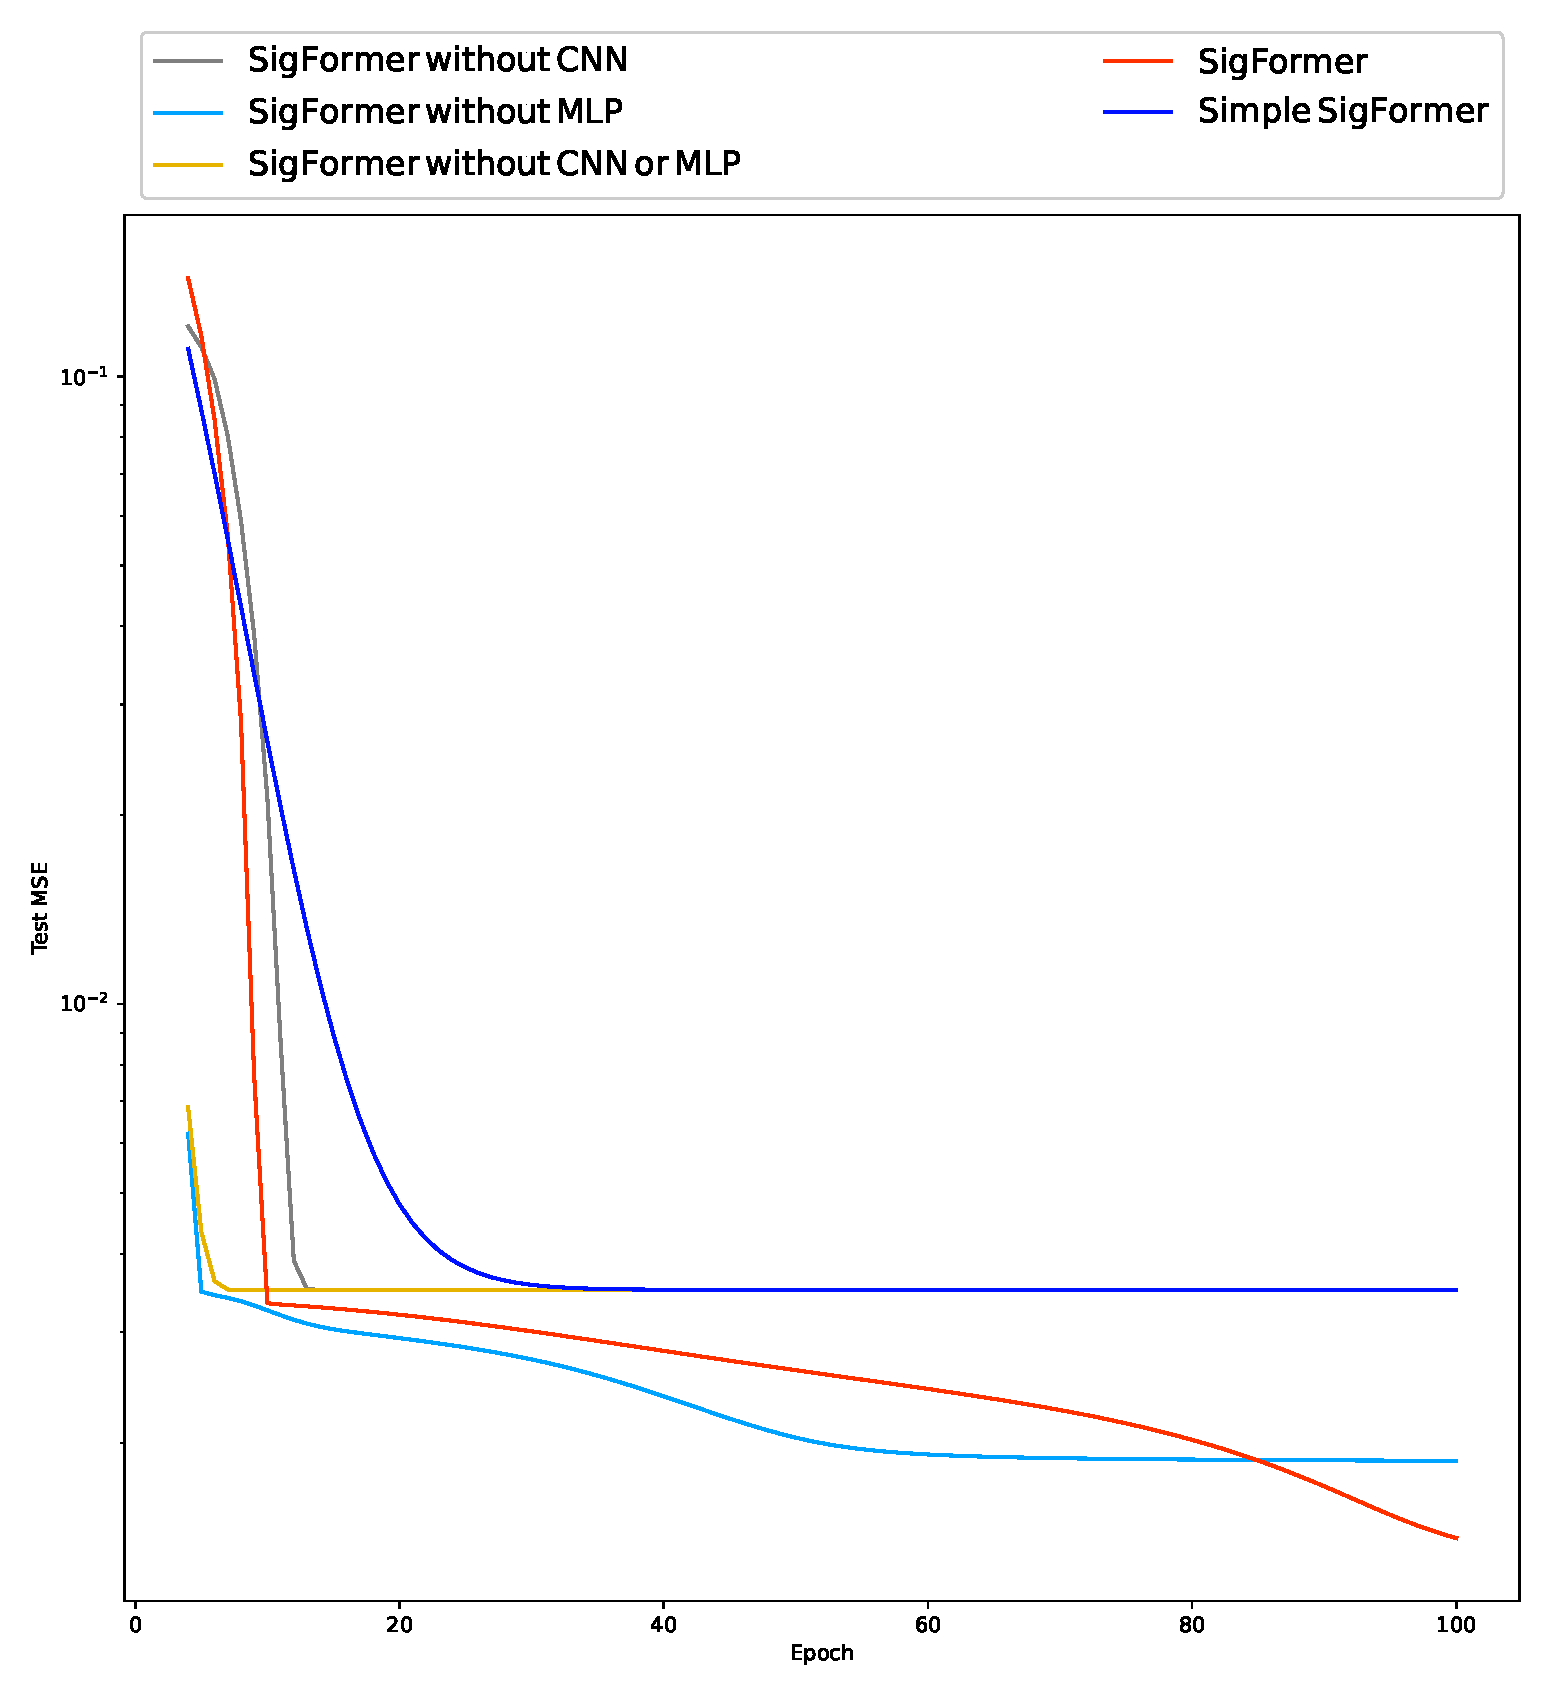
\includegraphics[width=0.32\textwidth]{fig//numerical_example3//loss_plots//beta//rBergomi_grid=200_Hbeta_eta=1_v0=0.01.eps}
			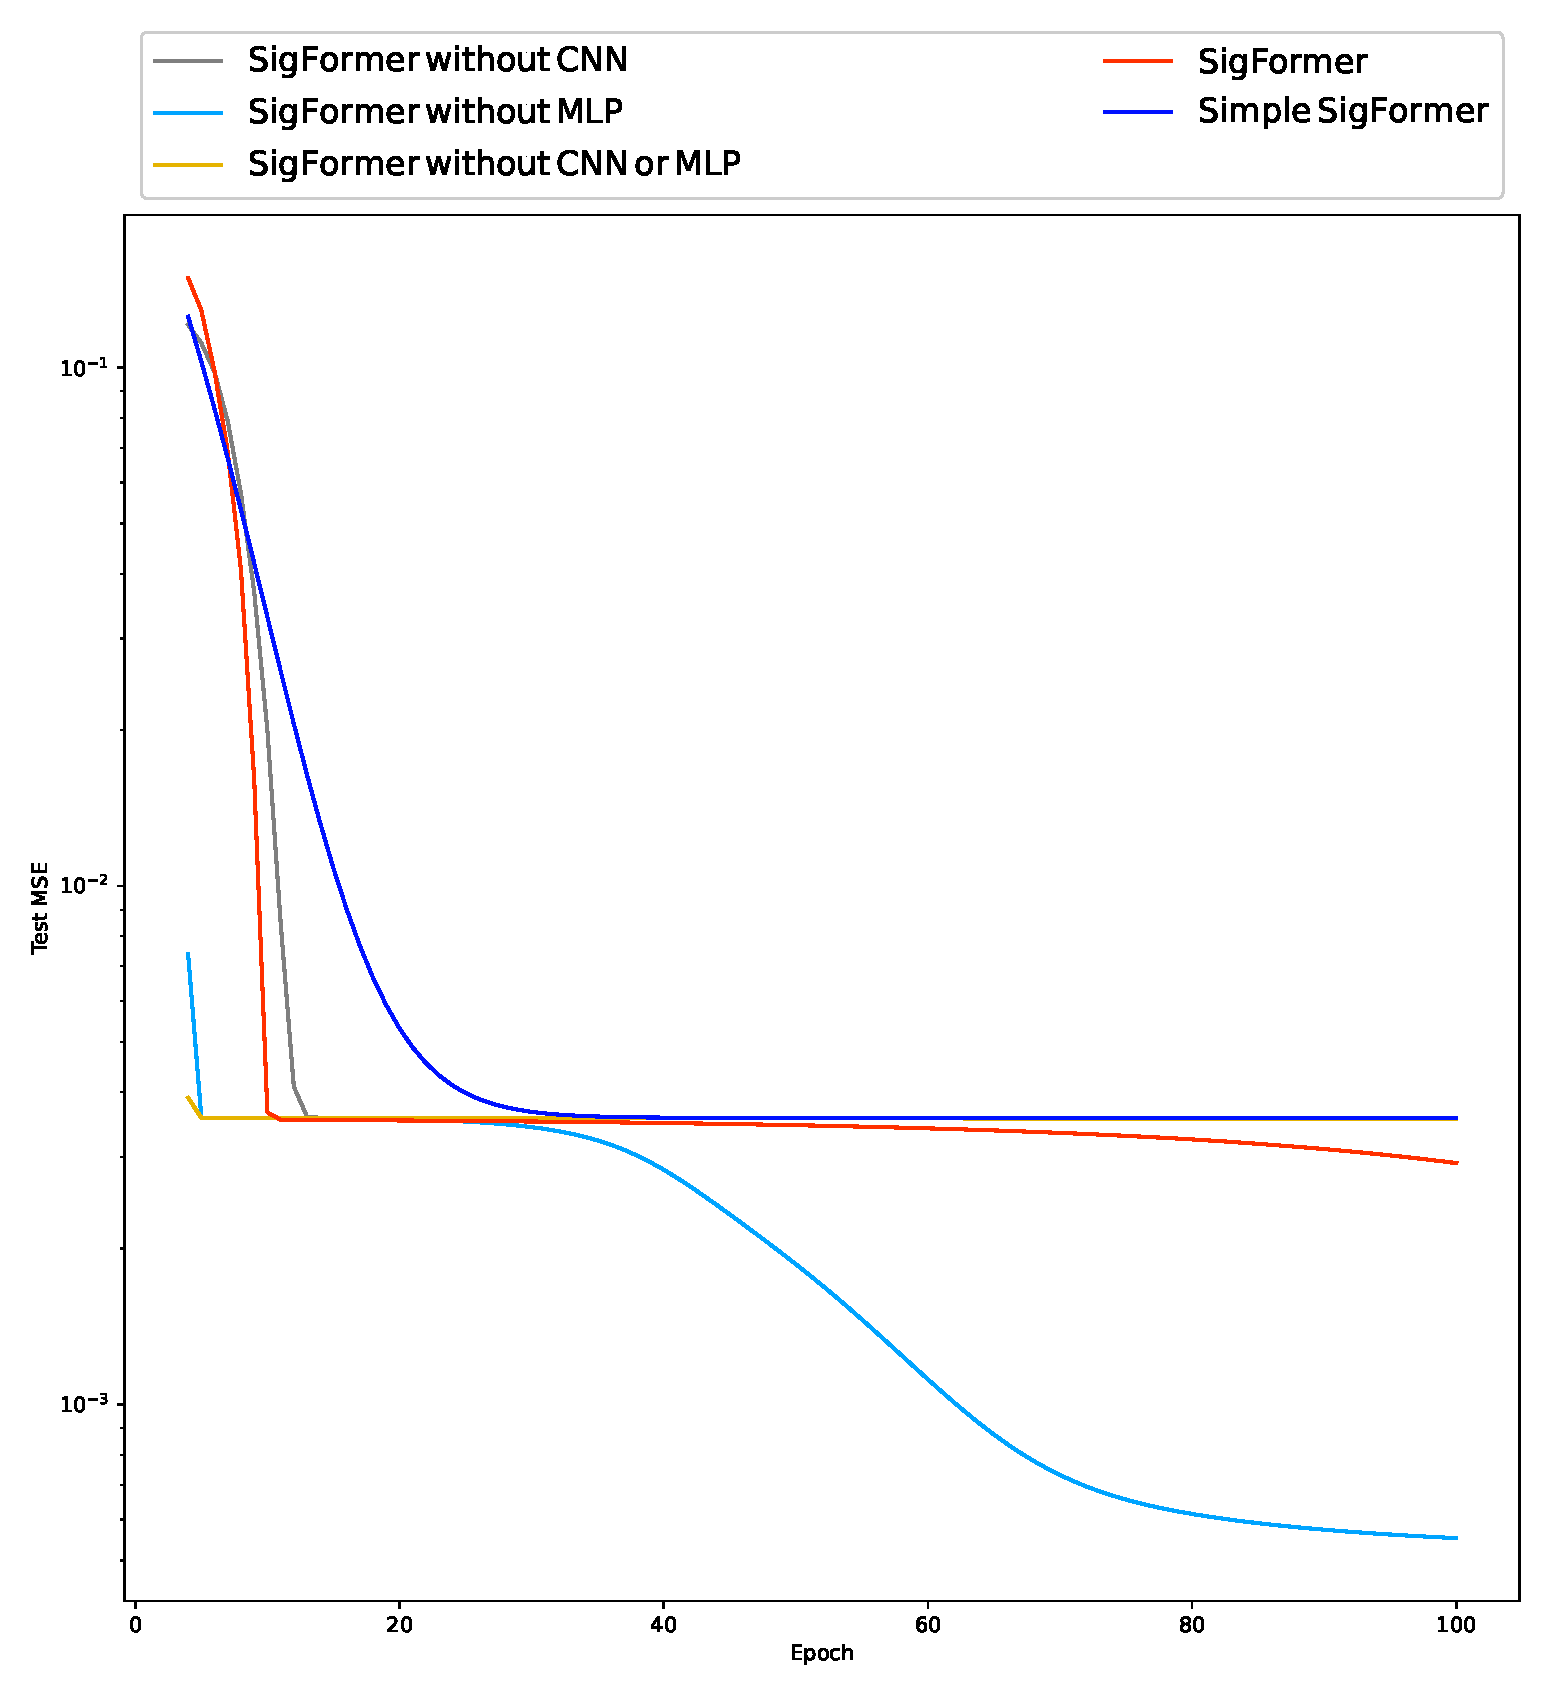
\includegraphics[width=0.32\textwidth]{fig//numerical_example3//loss_plots//beta//rHeston_grid=200_Hbeta_kappa1=0.1_kappa2=0.03_theta=0.3_v0=0.01.eps}}
	}
	\resizebox{0.9\textwidth}{!}{
		\subfigure[The input length equals to $300$.]{
			
\includegraphics[width=0.32\textwidth]{fig//numerical_example3//loss_plots//beta//fBm_grid=300_Hbeta.eps}
			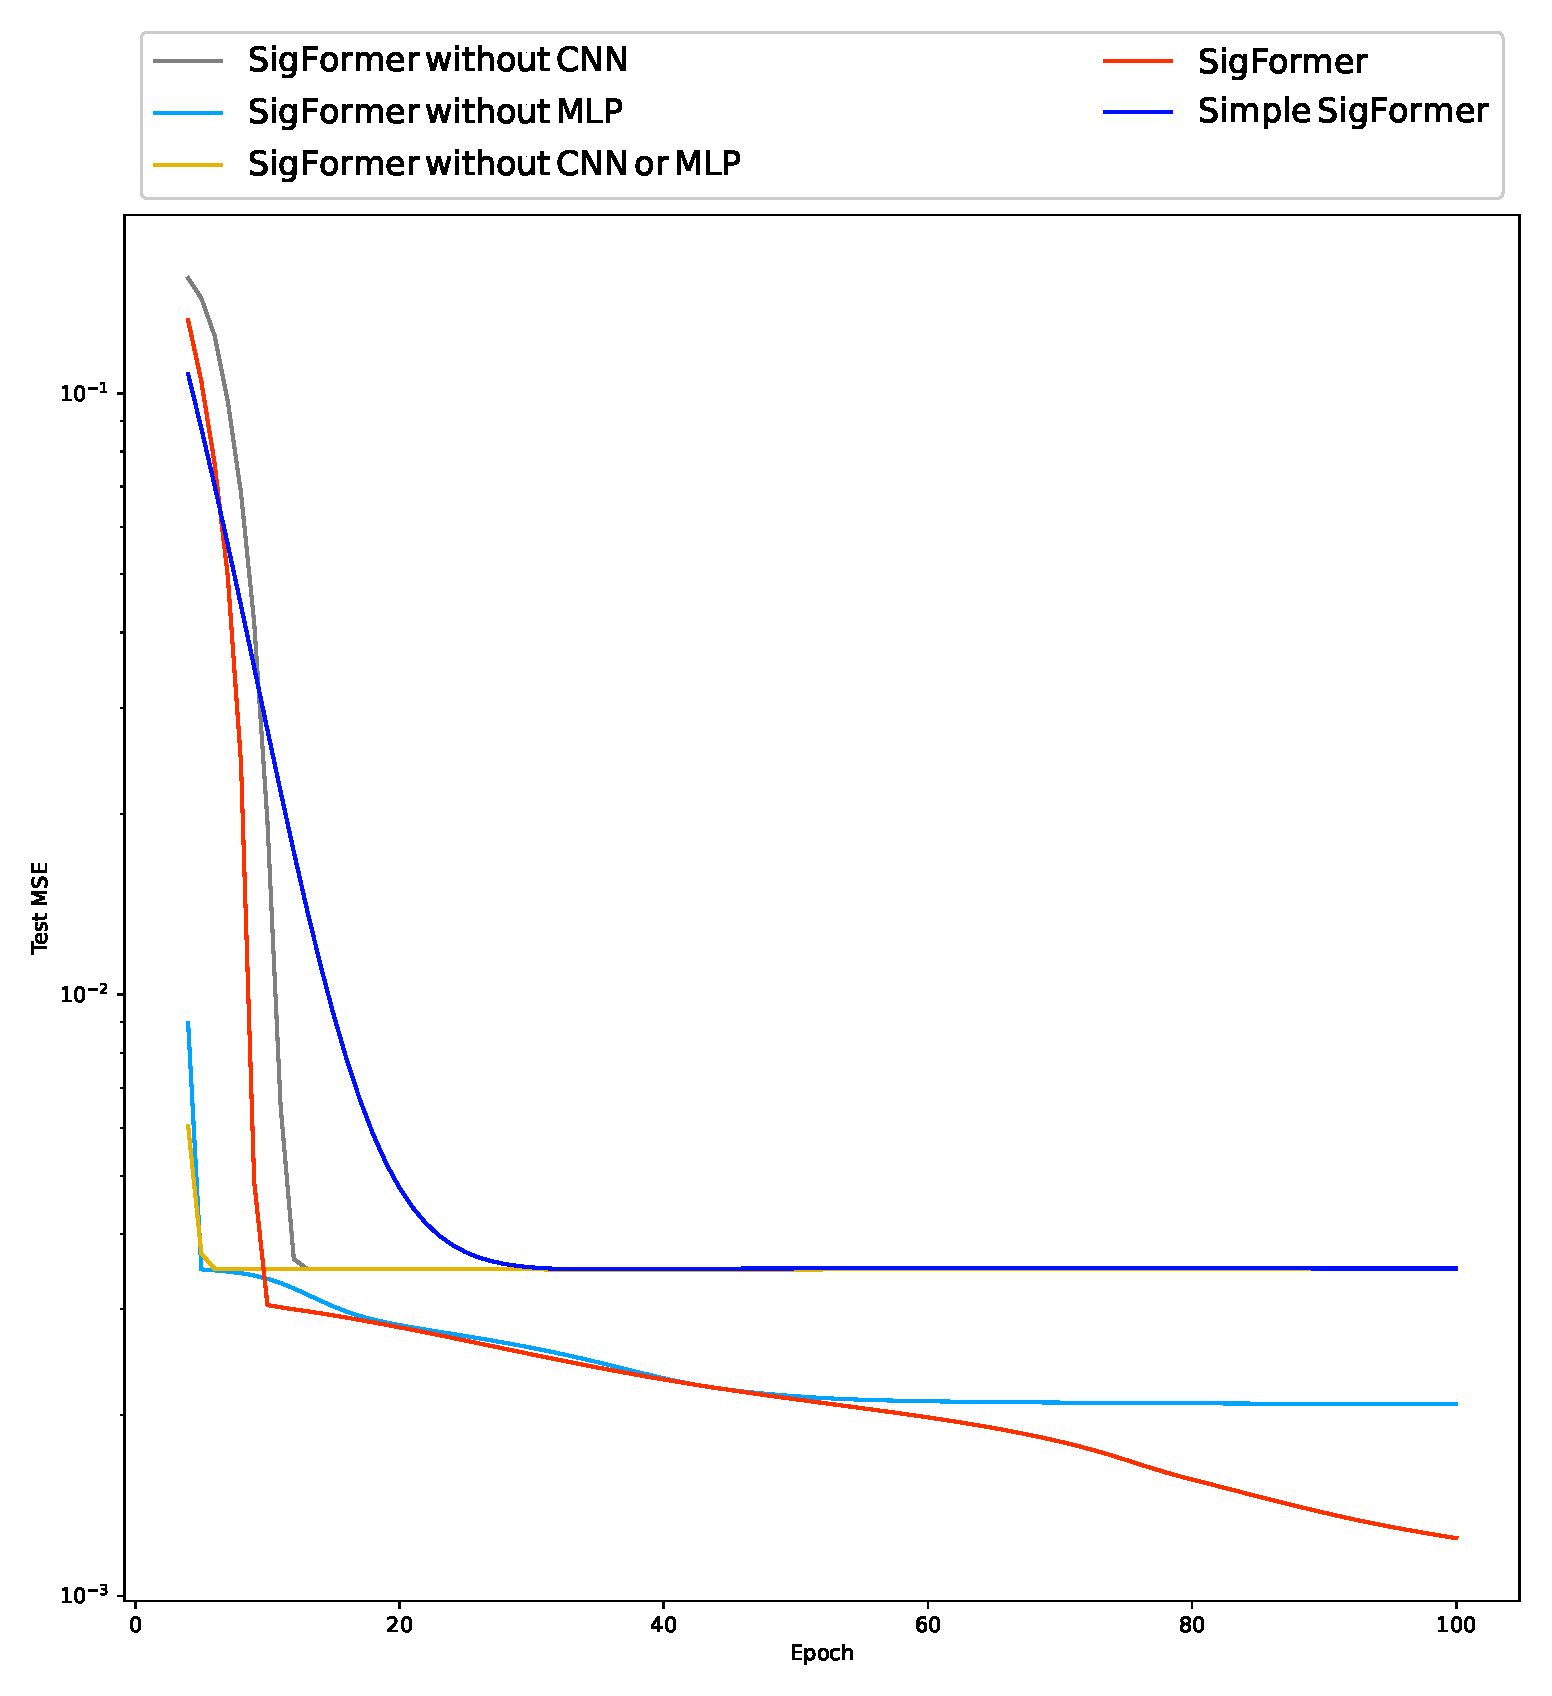
\includegraphics[width=0.32\textwidth]{fig//numerical_example3//loss_plots//beta//rBergomi_grid=300_Hbeta_eta=1_v0=0.01.eps}
			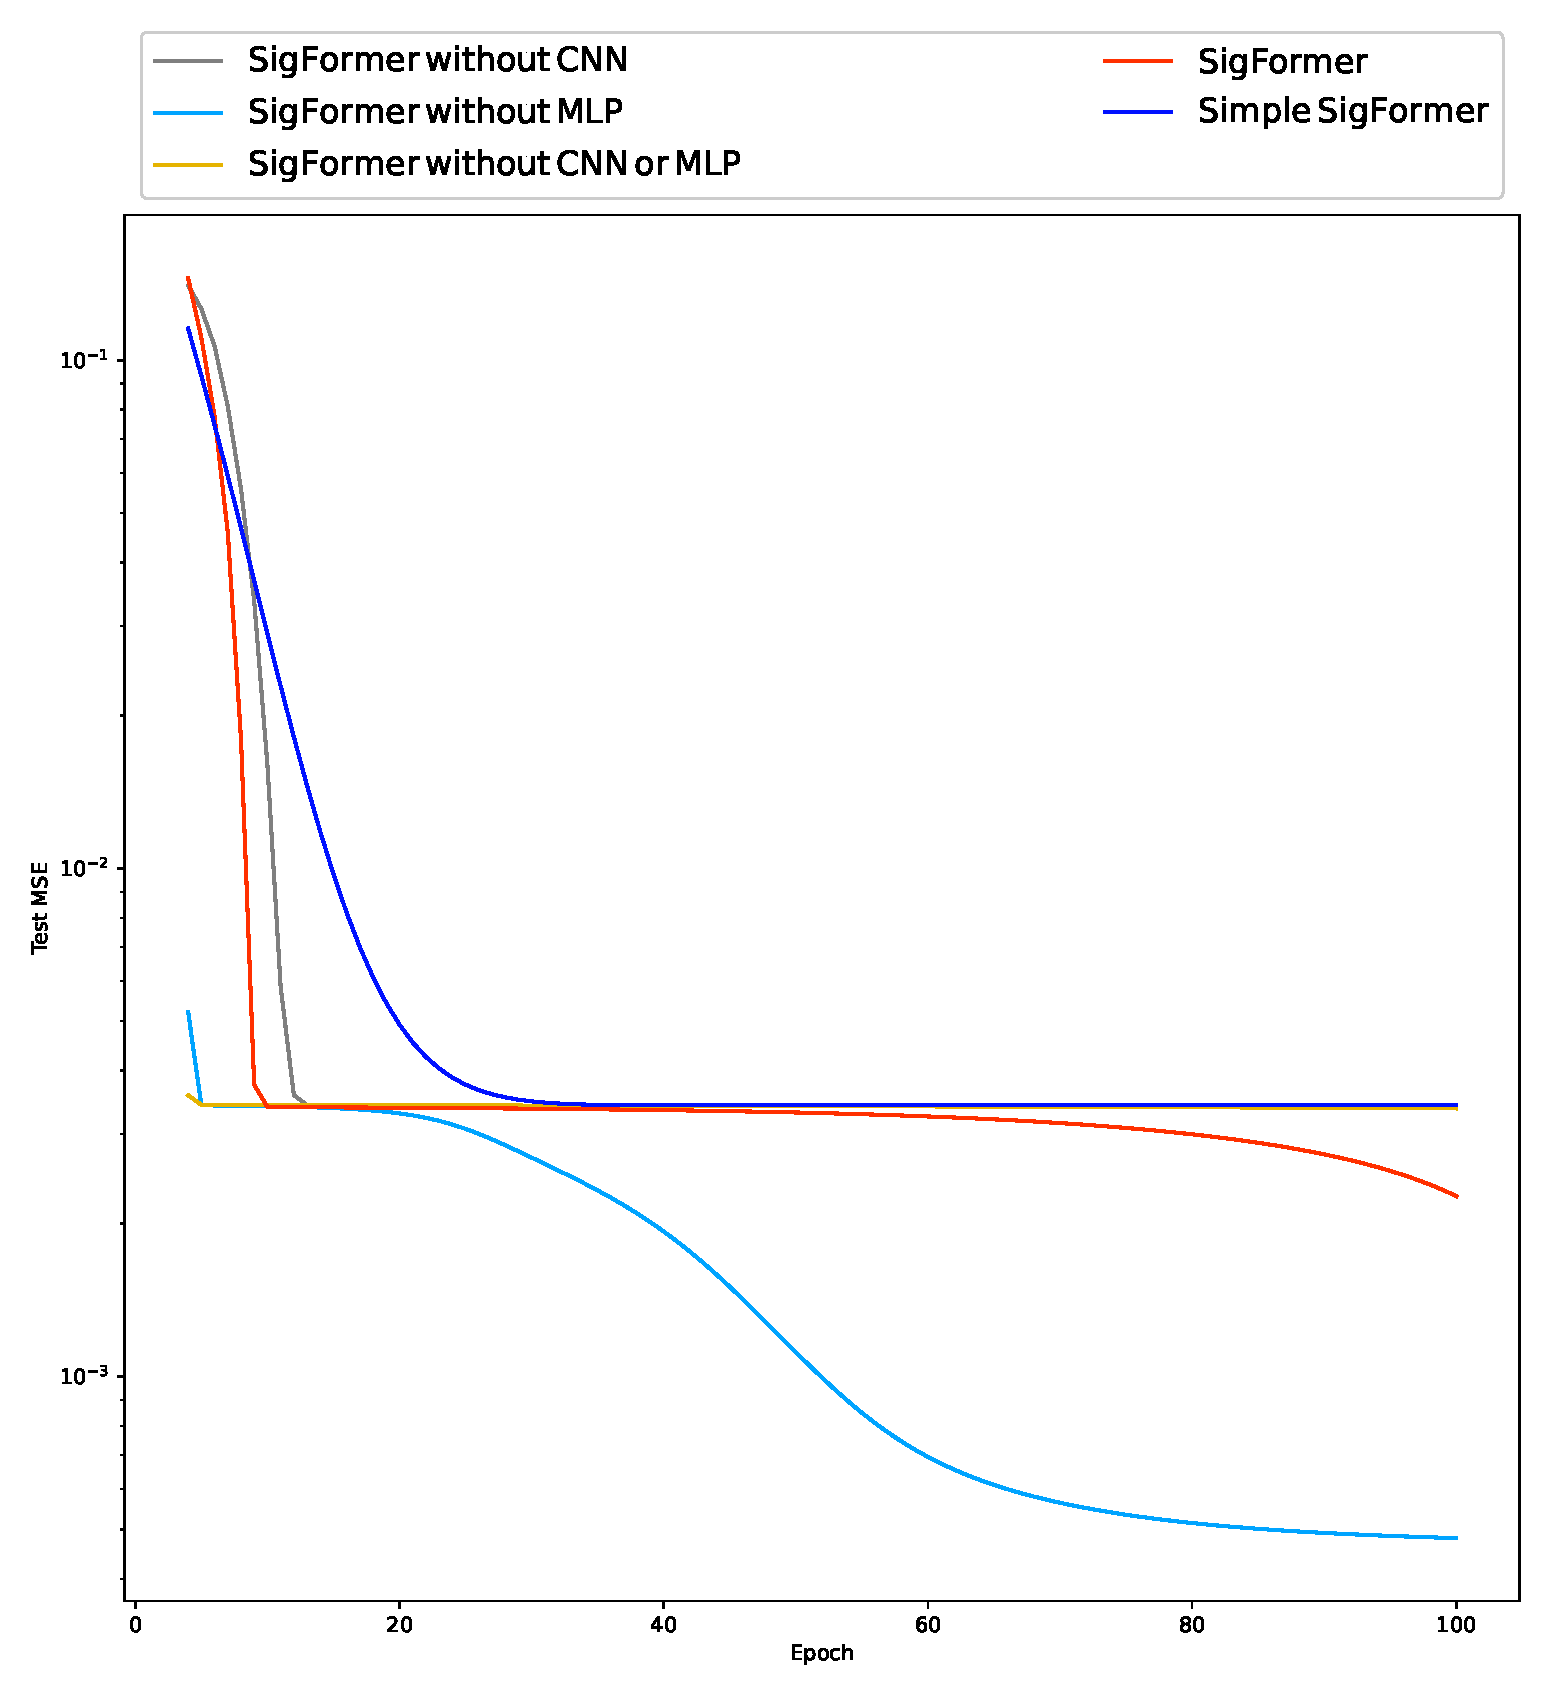
\includegraphics[width=0.32\textwidth]{fig//numerical_example3//loss_plots//beta//rHeston_grid=300_Hbeta_kappa1=0.1_kappa2=0.03_theta=0.3_v0=0.01.eps}}
	}
	\caption{Loss plot for (Left:) fBms; (Middle:) rBergomi volatility processes; (Right:) rHeston volatility processes with input lengths varying from $100$ to $300$ and $H\sim\text{Beta}(1,\,9)$. }
	\end{figure}
	
	\begin{figure}[H]
		\centering
		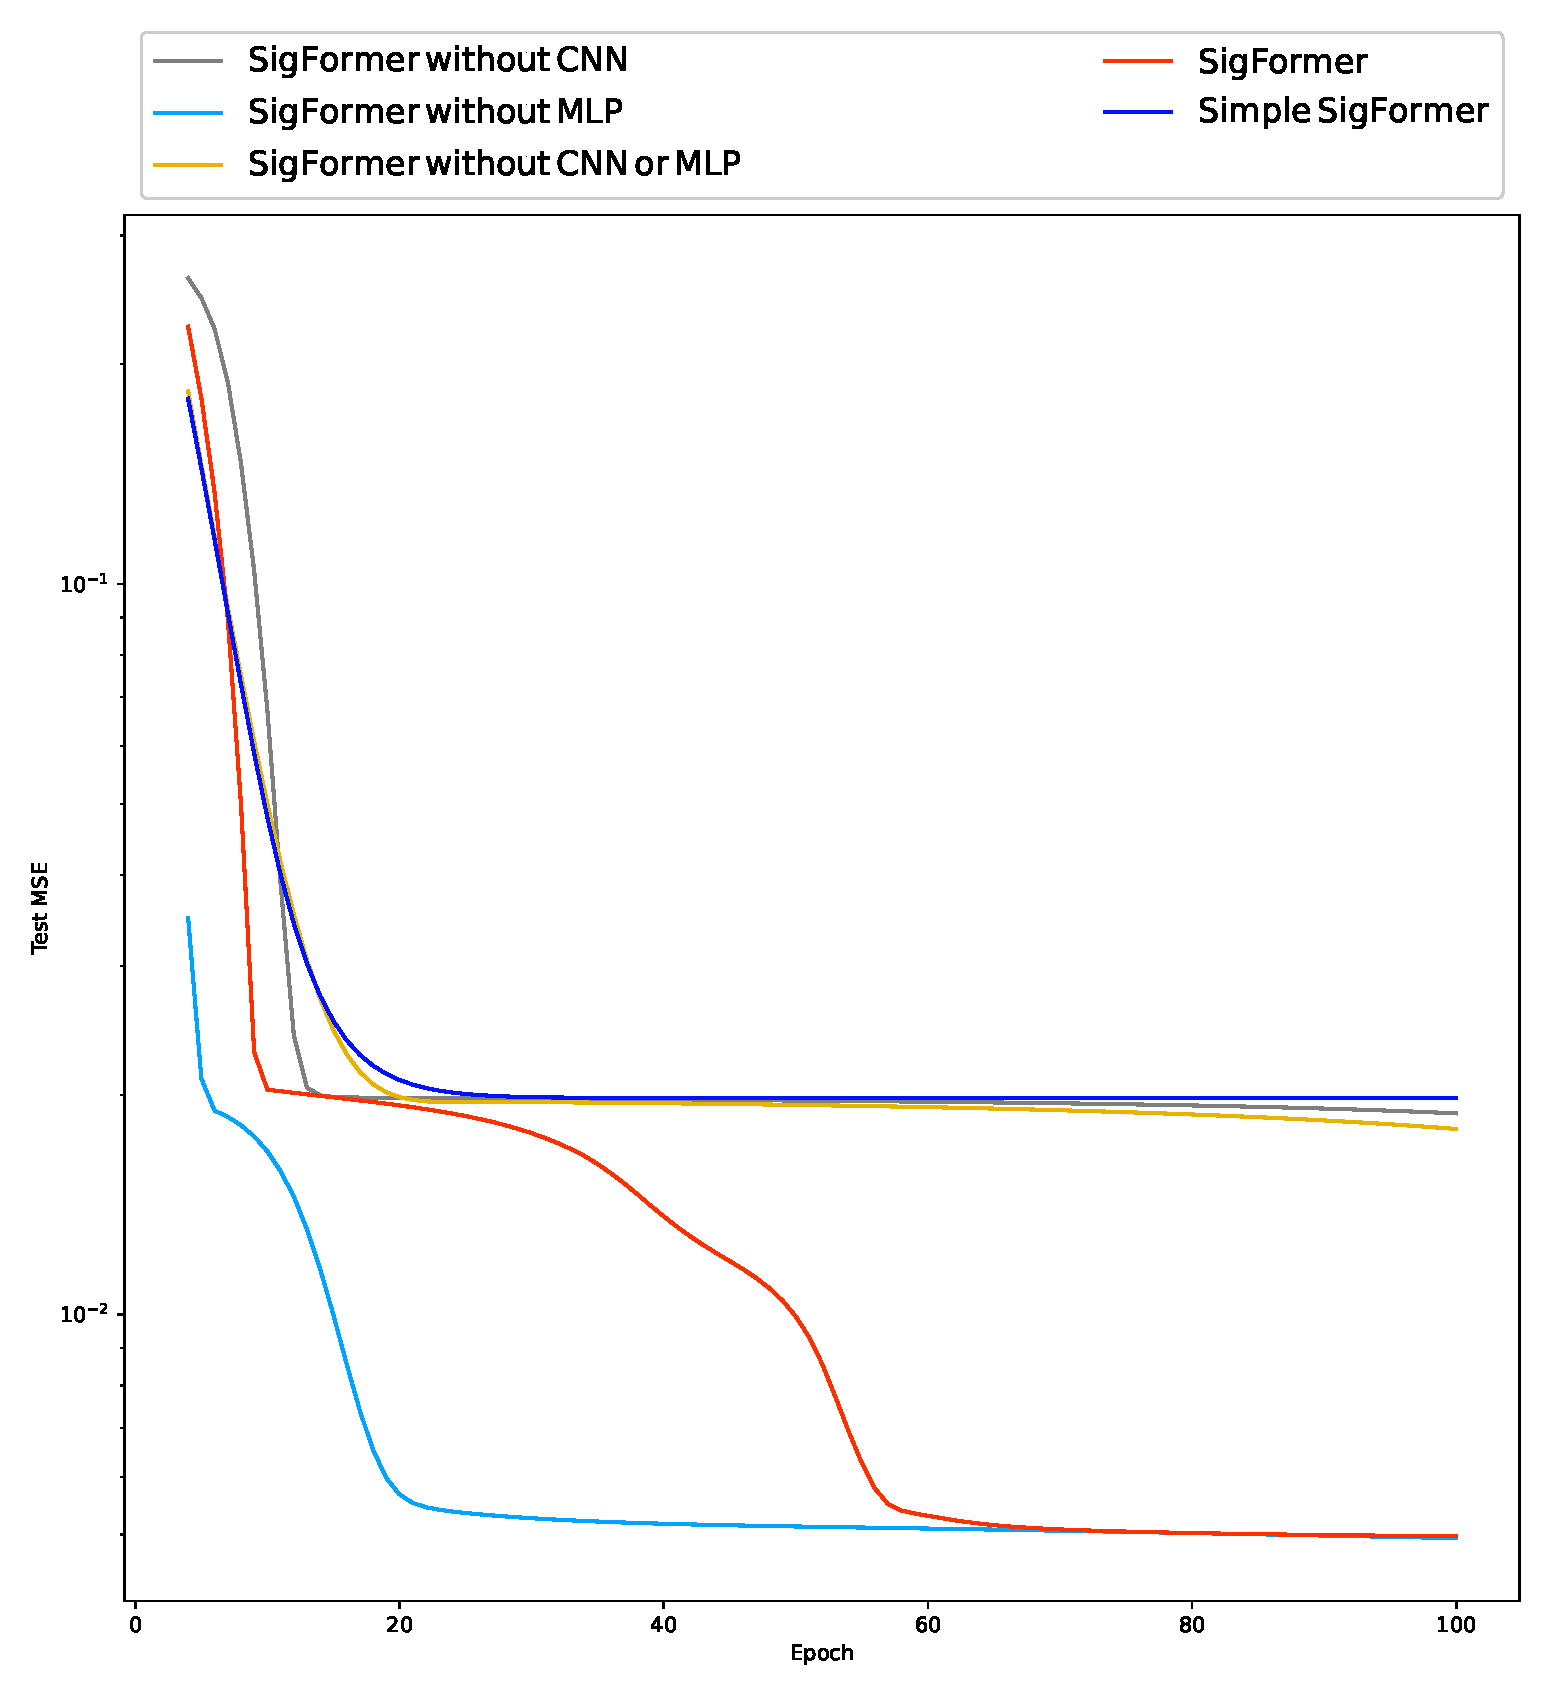
\includegraphics[width=0.32\textwidth]{fig//numerical_example3//loss_plots//multiple//rHeston_grid=100_Hbeta_kappa1=0.1_kappa2=0.03_thetauniform_v0=0.01.eps}
		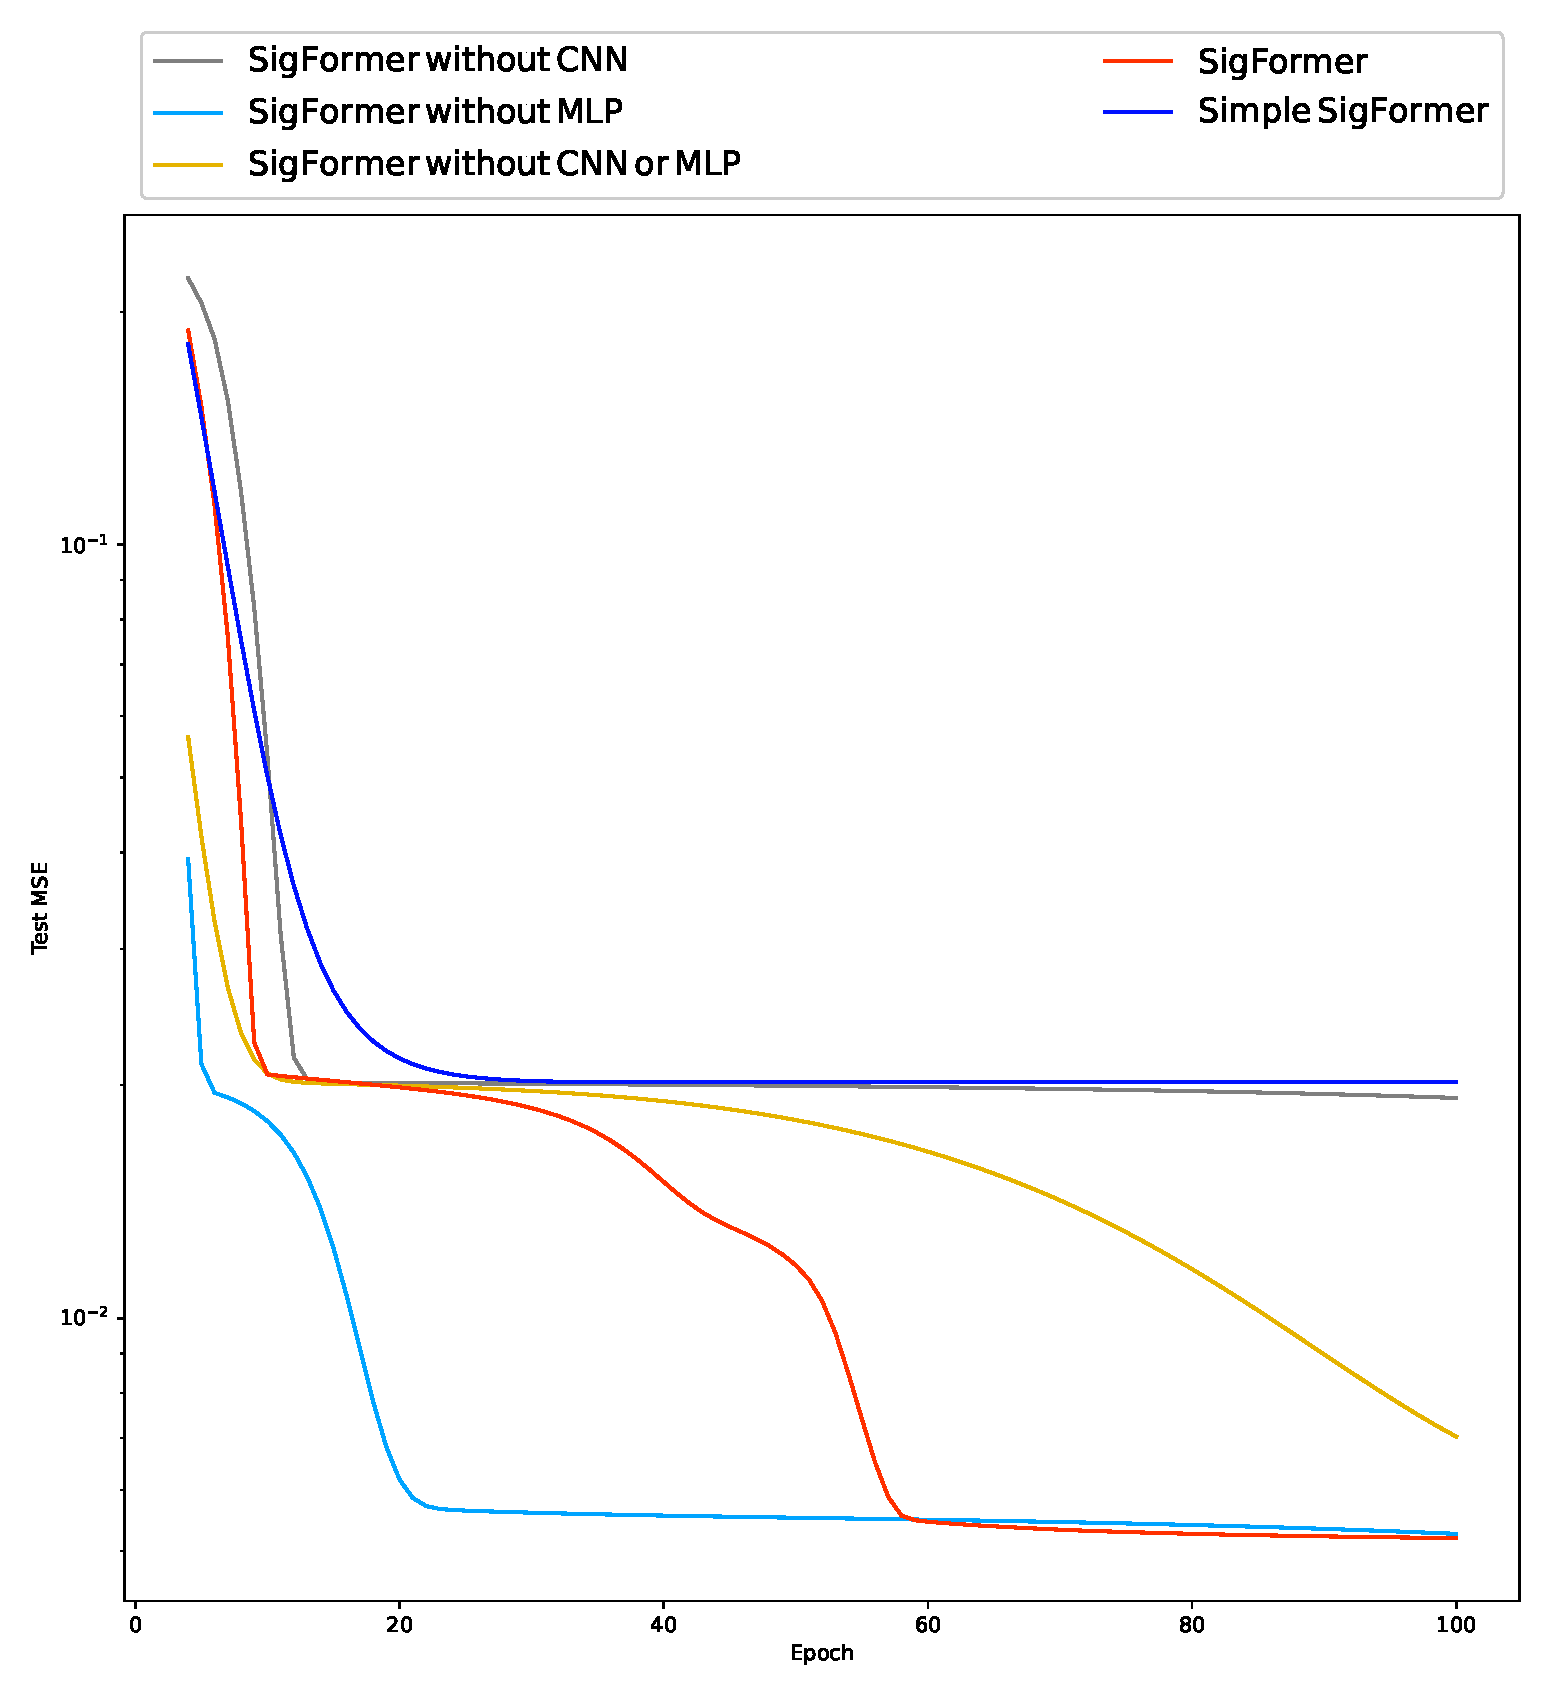
\includegraphics[width=0.32\textwidth]{fig//numerical_example3//loss_plots//multiple//rHeston_grid=200_Hbeta_kappa1=0.1_kappa2=0.03_thetauniform_v0=0.01.eps}
		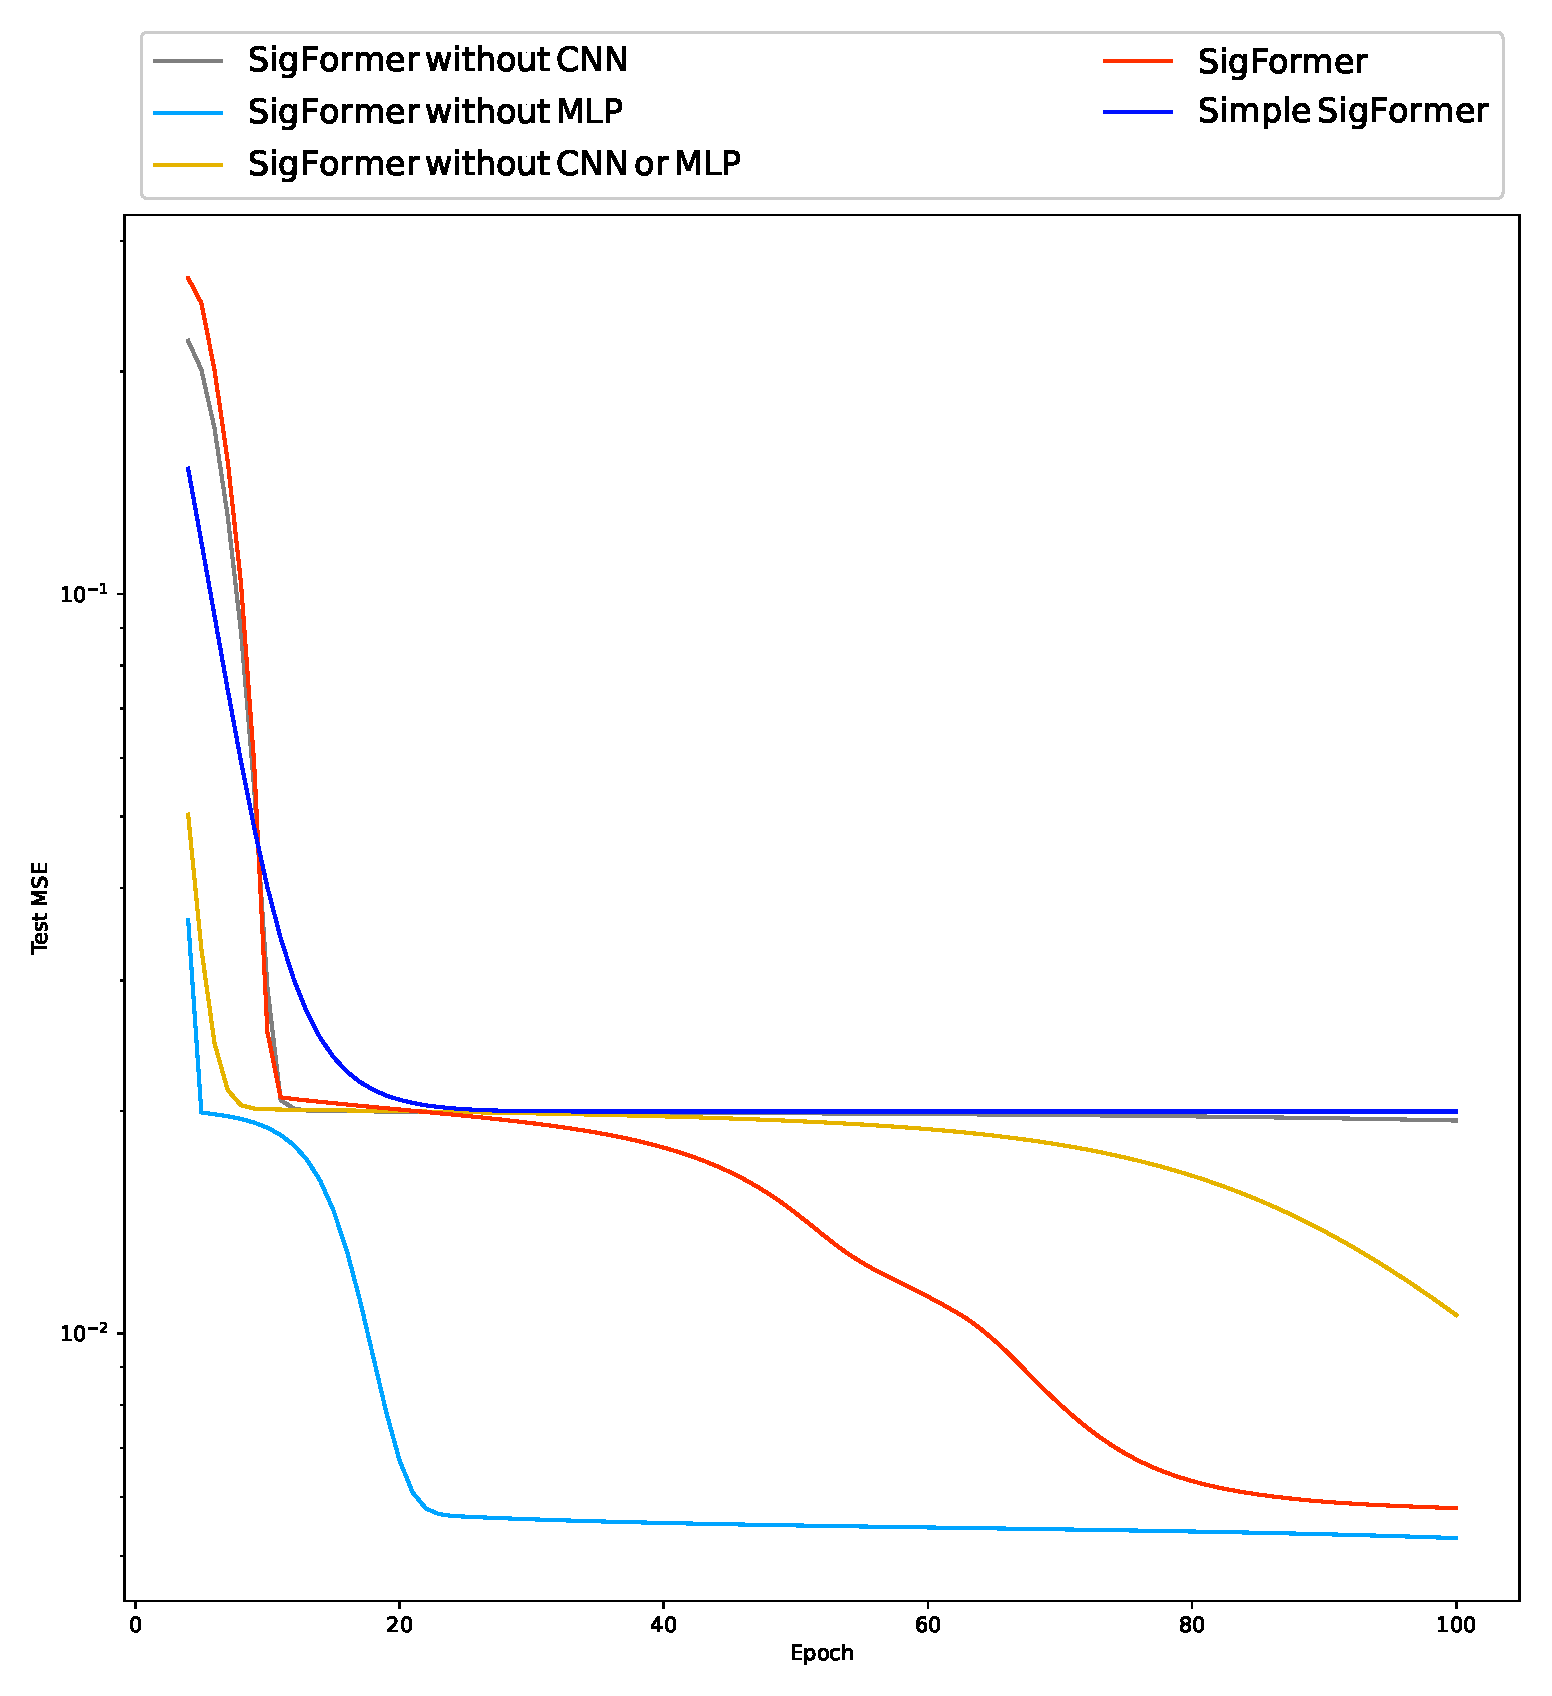
\includegraphics[width=0.32\textwidth]{fig//numerical_example3//loss_plots//multiple//rHeston_grid=300_Hbeta_kappa1=0.1_kappa2=0.03_thetauniform_v0=0.01.eps}
		\caption{Loss plot for rHeston volatility processes with input lengths varying from $100$ to $300$ (from left to right). Here, $H\sim\text{Beta}(1,\,9)$ and $\theta\sim\text{Uniform}(0,0.5)$. }
	\end{figure}
	
	\subsection{Loss plots for different models with input lengths varying from $100$ to $500$}
	\label{subapdix-loss-plots-calibration-single}
	\begin{figure}[H]
		\centering
		\resizebox{0.9\textwidth}{!}{
			\subfigure[$H\sim\text{Uniform}(0,0.5)$]{
				
\includegraphics[width=0.32\textwidth]{fig//numerical_example4//loss_plots//input_length_100//fBm_grid=100_Huniform.eps}
				
\includegraphics[width=0.32\textwidth]{fig//numerical_example4//loss_plots//input_length_100//rBergomi_grid=100_Huniform_eta=1_v0=0.01.eps}
				
\includegraphics[width=0.32\textwidth]{fig//numerical_example4//loss_plots//input_length_100//rHeston_grid=100_Huniform_kappa1=0.1_kappa2=0.03_theta=0.3_v0=0.01.eps}}
		}
		\resizebox{0.9\textwidth}{!}{
			\subfigure[$H\sim\text{Beta}(1,\,9)$]{
				
\includegraphics[width=0.32\textwidth]{fig//numerical_example4//loss_plots//input_length_100//fBm_grid=100_Hbeta.eps}
				
\includegraphics[width=0.32\textwidth]{fig//numerical_example4//loss_plots//input_length_100//rBergomi_grid=100_Hbeta_eta=1_v0=0.01.eps}
				
\includegraphics[width=0.32\textwidth]{fig//numerical_example4//loss_plots//input_length_100//rHeston_grid=100_Hbeta_kappa1=0.1_kappa2=0.03_theta=0.3_v0=0.01.eps}}
		}
		\caption{Loss plot for (Left:) fBms; (Middle:) rBergomi volatility processes; (Right:) rHeston volatility processes with input lengths equal to $100$. }
	\end{figure}
	
	\begin{figure}[H]
		\centering
		\resizebox{0.9\textwidth}{!}{
			\subfigure[$H\sim\text{Uniform}(0,0.5)$]{
				
\includegraphics[width=0.32\textwidth]{fig//numerical_example4//loss_plots//input_length_200//fBm_grid=200_Huniform.eps}
				
\includegraphics[width=0.32\textwidth]{fig//numerical_example4//loss_plots//input_length_200//rBergomi_grid=200_Huniform_eta=1_v0=0.01.eps}
				
\includegraphics[width=0.32\textwidth]{fig//numerical_example4//loss_plots//input_length_200//rHeston_grid=200_Huniform_kappa1=0.1_kappa2=0.03_theta=0.3_v0=0.01.eps}}
		}
		\resizebox{0.9\textwidth}{!}{
			\subfigure[$H\sim\text{Beta}(1,\,9)$]{
				
\includegraphics[width=0.32\textwidth]{fig//numerical_example4//loss_plots//input_length_200//fBm_grid=200_Hbeta.eps}
				
\includegraphics[width=0.32\textwidth]{fig//numerical_example4//loss_plots//input_length_200//rBergomi_grid=200_Hbeta_eta=1_v0=0.01.eps}
				
\includegraphics[width=0.32\textwidth]{fig//numerical_example4//loss_plots//input_length_200//rHeston_grid=200_Hbeta_kappa1=0.1_kappa2=0.03_theta=0.3_v0=0.01.eps}}
		}
		\caption{Loss plot for (Left:) fBms; (Middle:) rBergomi volatility processes; (Right:) rHeston volatility processes with input lengths equal to $200$. }
	\end{figure}
	
	\begin{figure}[H]
		\centering
		\resizebox{0.9\textwidth}{!}{
			\subfigure[$H\sim\text{Uniform}(0,0.5)$]{
				
\includegraphics[width=0.32\textwidth]{fig//numerical_example4//loss_plots//input_length_300//fBm_grid=300_Huniform.eps}
				
\includegraphics[width=0.32\textwidth]{fig//numerical_example4//loss_plots//input_length_300//rBergomi_grid=300_Huniform_eta=1_v0=0.01.eps}
				
\includegraphics[width=0.32\textwidth]{fig//numerical_example4//loss_plots//input_length_300//rHeston_grid=300_Huniform_kappa1=0.1_kappa2=0.03_theta=0.3_v0=0.01.eps}}
		}
		\resizebox{0.9\textwidth}{!}{
			\subfigure[$H\sim\text{Beta}(1,\,9)$]{
				
\includegraphics[width=0.32\textwidth]{fig//numerical_example4//loss_plots//input_length_300//fBm_grid=300_Hbeta.eps}
				
\includegraphics[width=0.32\textwidth]{fig//numerical_example4//loss_plots//input_length_300//rBergomi_grid=300_Hbeta_eta=1_v0=0.01.eps}
				
\includegraphics[width=0.32\textwidth]{fig//numerical_example4//loss_plots//input_length_300//rHeston_grid=300_Hbeta_kappa1=0.1_kappa2=0.03_theta=0.3_v0=0.01.eps}}
		}
		\caption{Loss plot for (Left:) fBms; (Middle:) rBergomi volatility processes; (Right:) rHeston volatility processes with input lengths equal to $300$. }
	\end{figure}
	
	\begin{figure}[H]
		\centering
		\resizebox{0.9\textwidth}{!}{
			\subfigure[$H\sim\text{Uniform}(0,0.5)$]{
				
\includegraphics[width=0.32\textwidth]{fig//numerical_example4//loss_plots//input_length_400//fBm_grid=400_Huniform.eps}
				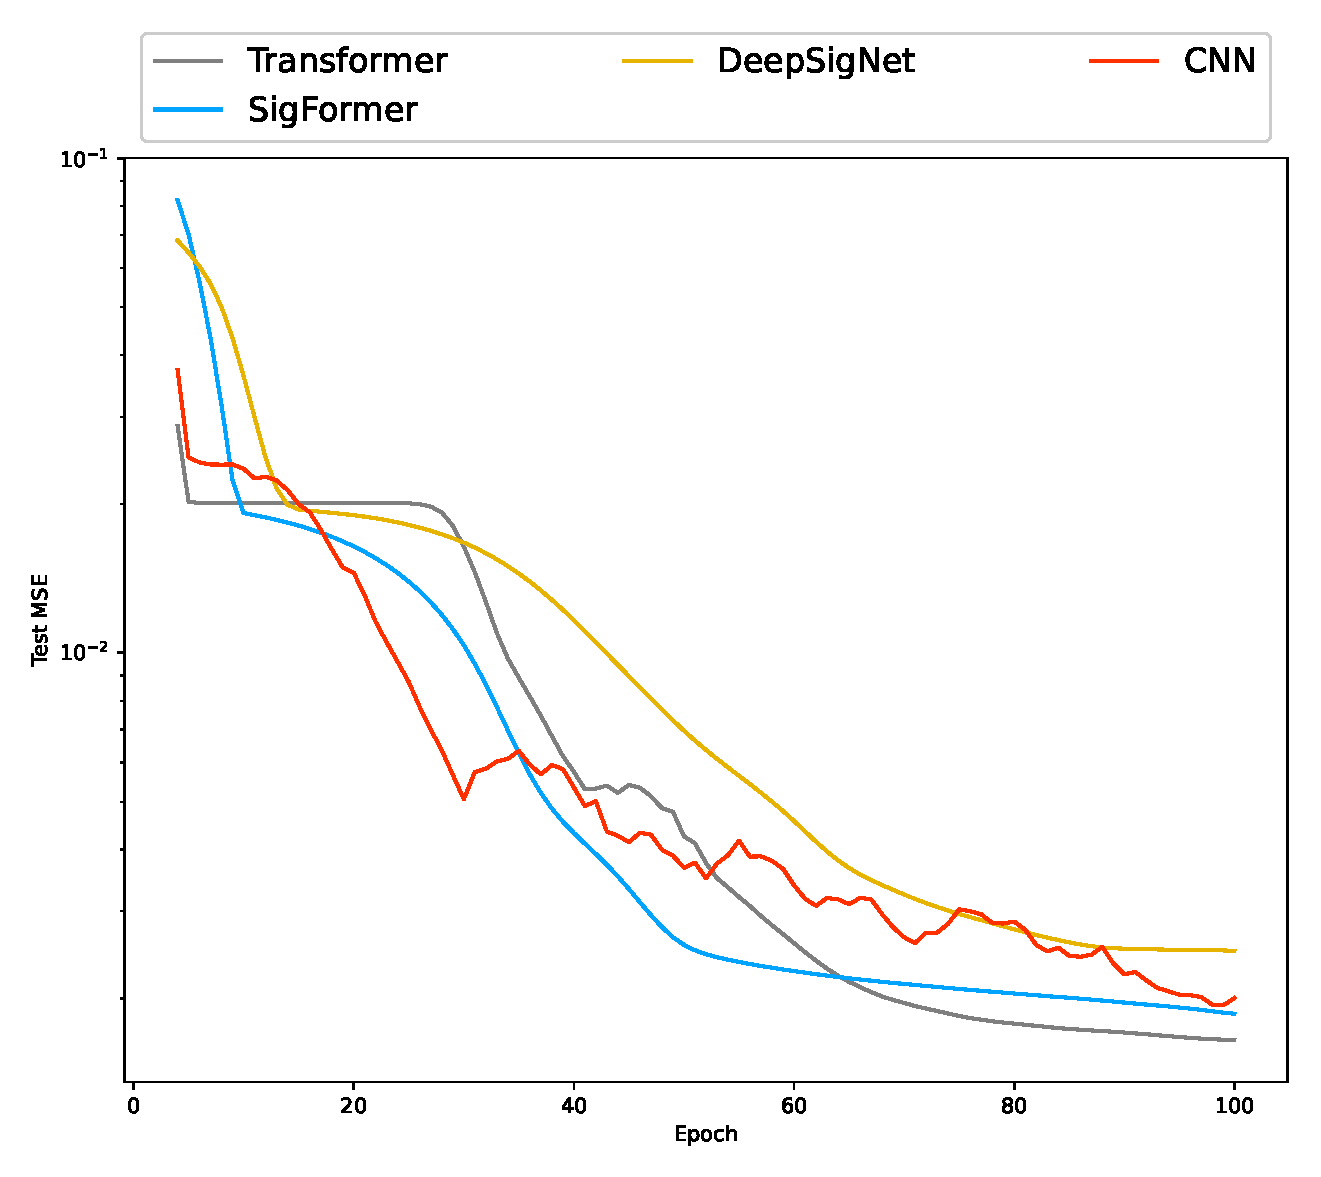
\includegraphics[width=0.32\textwidth]{fig//numerical_example4//loss_plots//input_length_400//rBergomi_grid=400_Huniform_eta=1_v0=0.01.eps}
				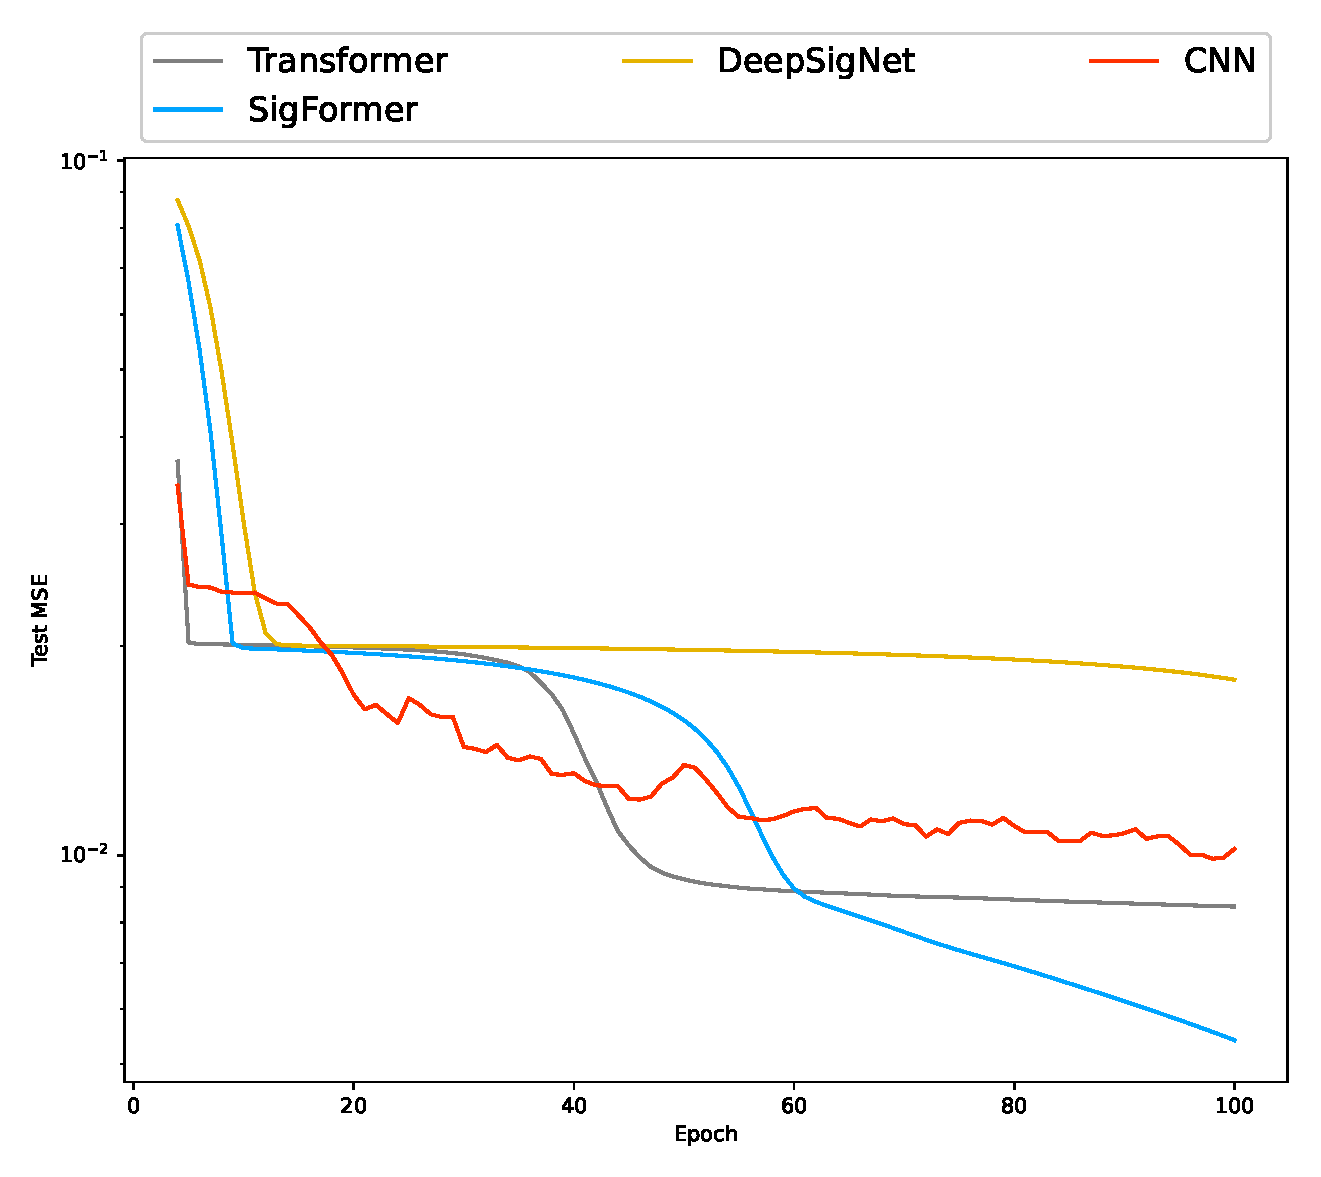
\includegraphics[width=0.32\textwidth]{fig//numerical_example4//loss_plots//input_length_400//rHeston_grid=400_Huniform_kappa1=0.1_kappa2=0.03_theta=0.3_v0=0.01.eps}}
		}
		\resizebox{0.9\textwidth}{!}{
			\subfigure[$H\sim\text{Beta}(1,\,9)$]{
				
\includegraphics[width=0.32\textwidth]{fig//numerical_example4//loss_plots//input_length_400//fBm_grid=400_Hbeta.eps}
				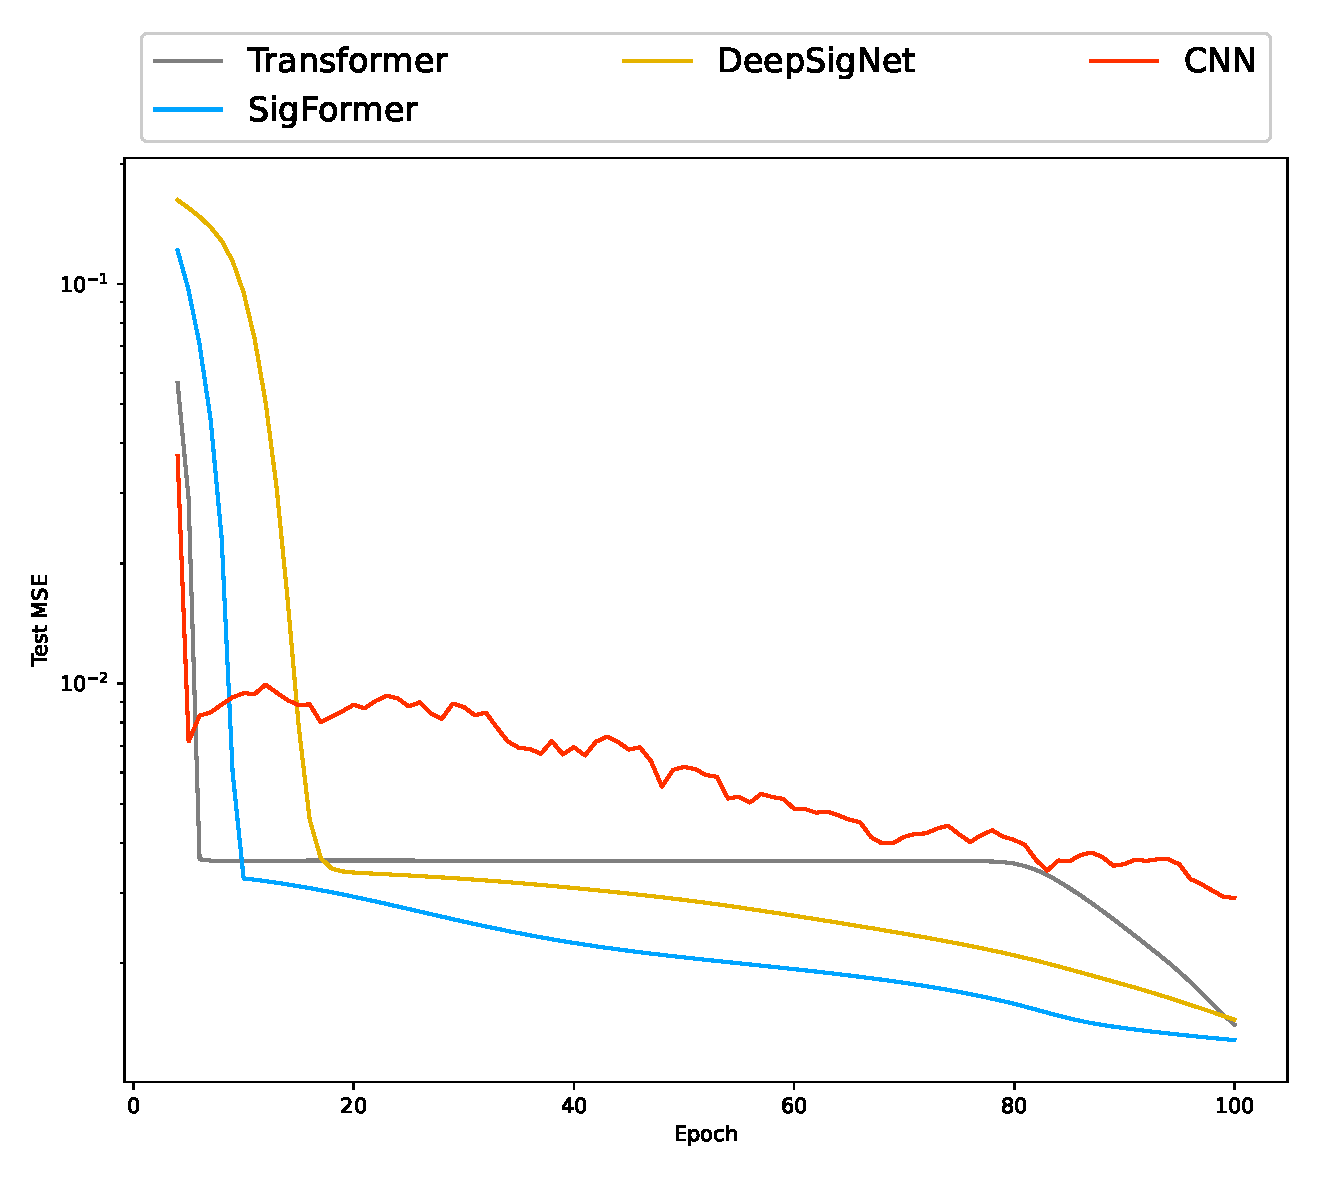
\includegraphics[width=0.32\textwidth]{fig//numerical_example4//loss_plots//input_length_400//rBergomi_grid=400_Hbeta_eta=1_v0=0.01.eps}
				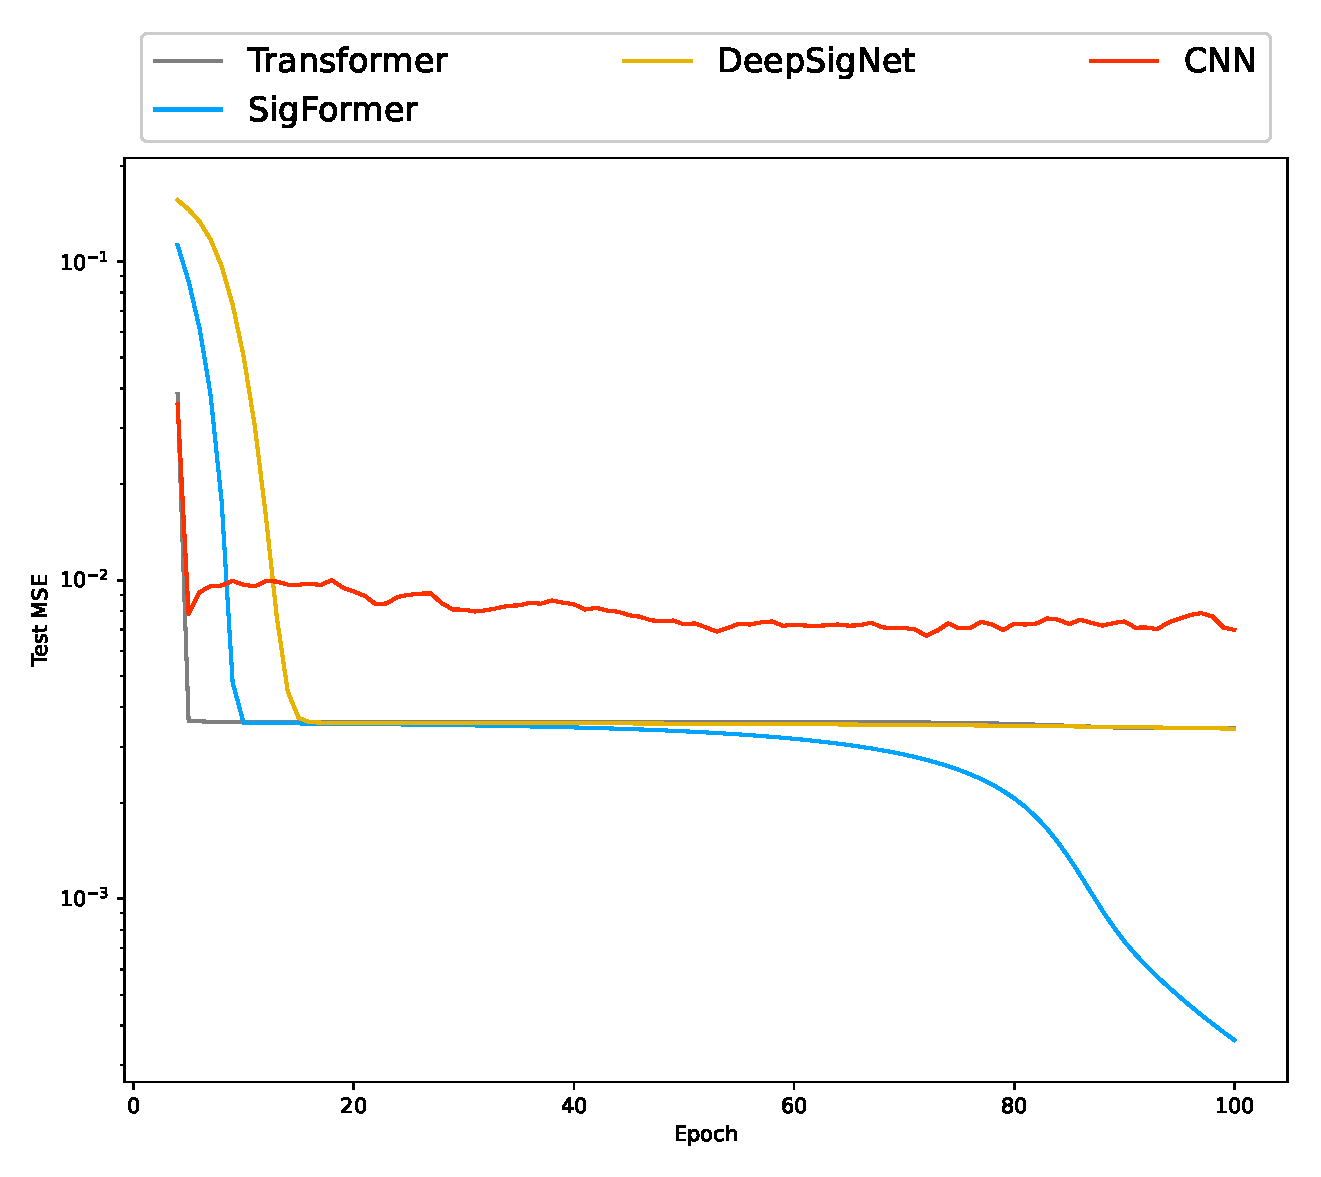
\includegraphics[width=0.32\textwidth]{fig//numerical_example4//loss_plots//input_length_400//rHeston_grid=400_Hbeta_kappa1=0.1_kappa2=0.03_theta=0.3_v0=0.01.eps}}
		}
		\caption{Loss plot for (Left:) fBms; (Middle:) rBergomi volatility processes; (Right:) rHeston volatility processes with input lengths equal to $400$. }
	\end{figure}
	
	\begin{figure}[H]
		\centering
		\resizebox{0.9\textwidth}{!}{
			\subfigure[$H\sim\text{Uniform}(0,0.5)$]{
				
\includegraphics[width=0.32\textwidth]{fig//numerical_example4//loss_plots//input_length_500//fBm_grid=500_Huniform.eps}
				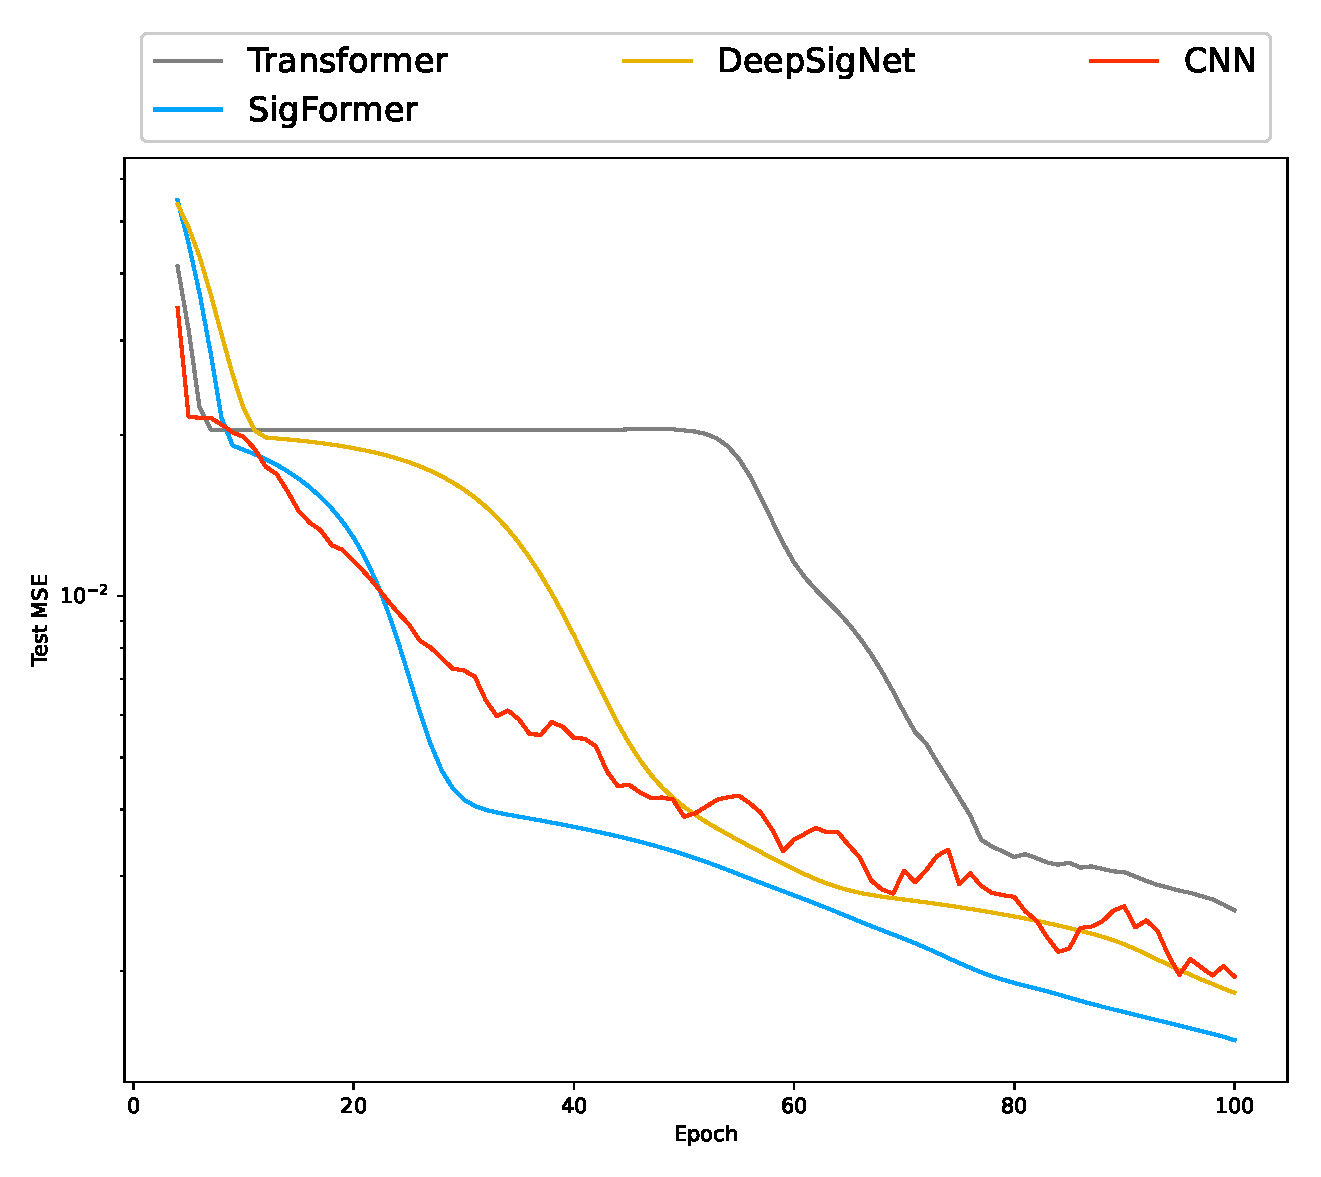
\includegraphics[width=0.32\textwidth]{fig//numerical_example4//loss_plots//input_length_500//rBergomi_grid=500_Huniform_eta=1_v0=0.01.eps}
				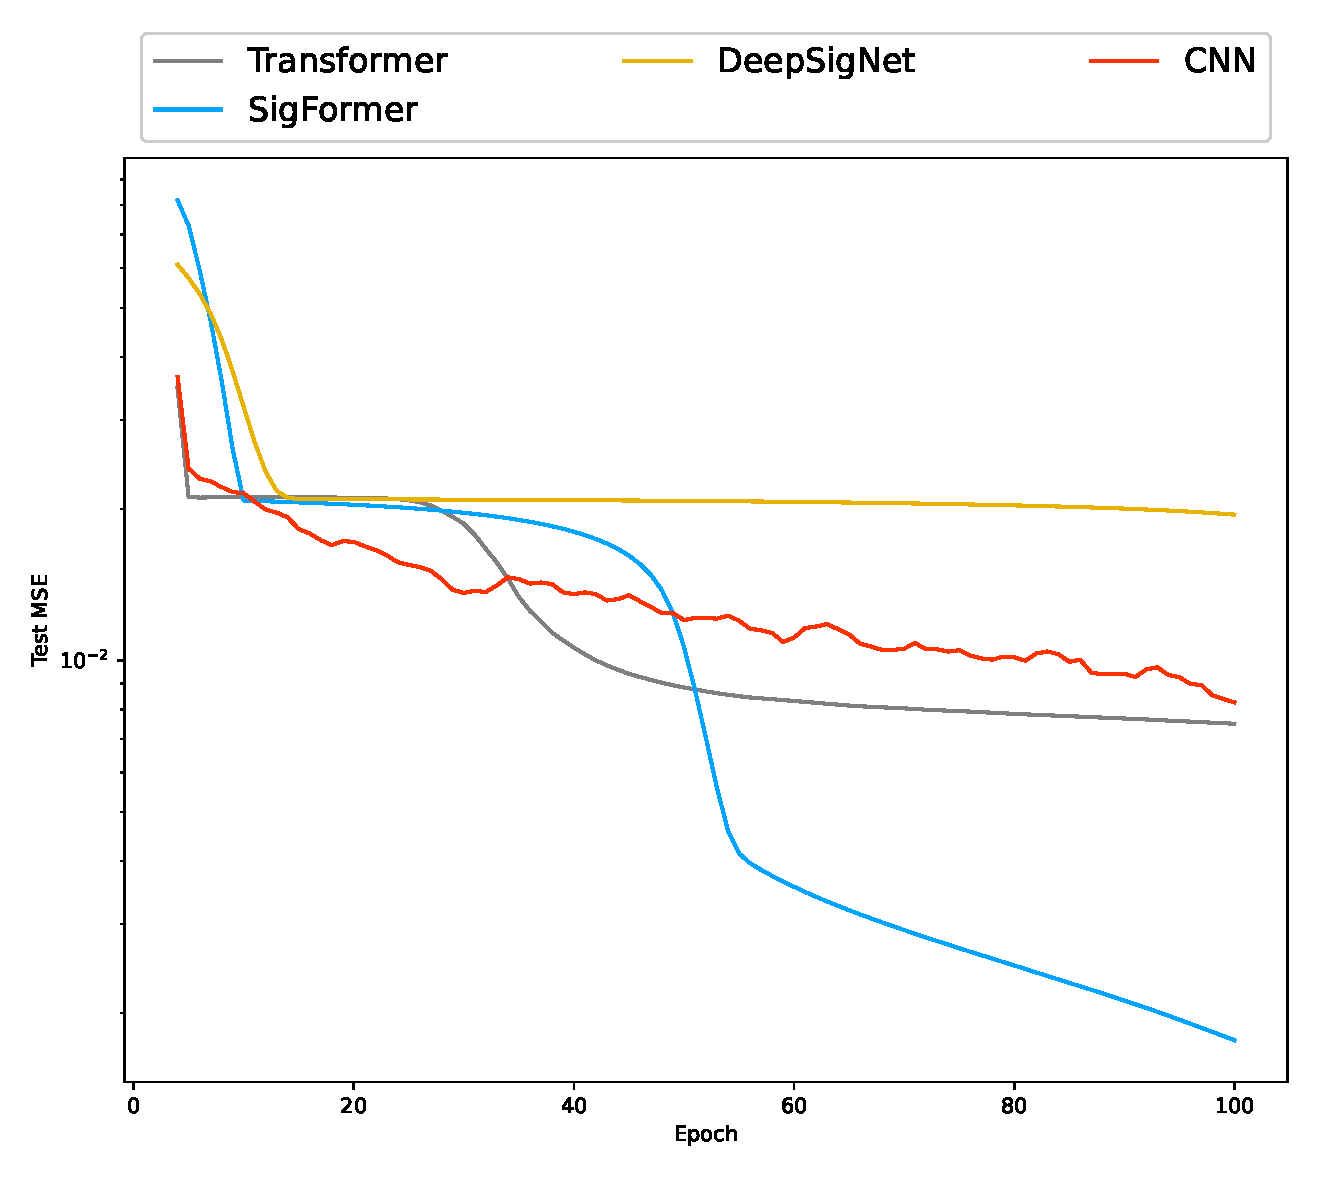
\includegraphics[width=0.32\textwidth]{fig//numerical_example4//loss_plots//input_length_500//rHeston_grid=500_Huniform_kappa1=0.1_kappa2=0.03_theta=0.3_v0=0.01.eps}}
		}
		\resizebox{0.9\textwidth}{!}{
			\subfigure[$H\sim\text{Beta}(1,\,9)$]{
				
\includegraphics[width=0.32\textwidth]{fig//numerical_example4//loss_plots//input_length_500//fBm_grid=500_Hbeta.eps}
				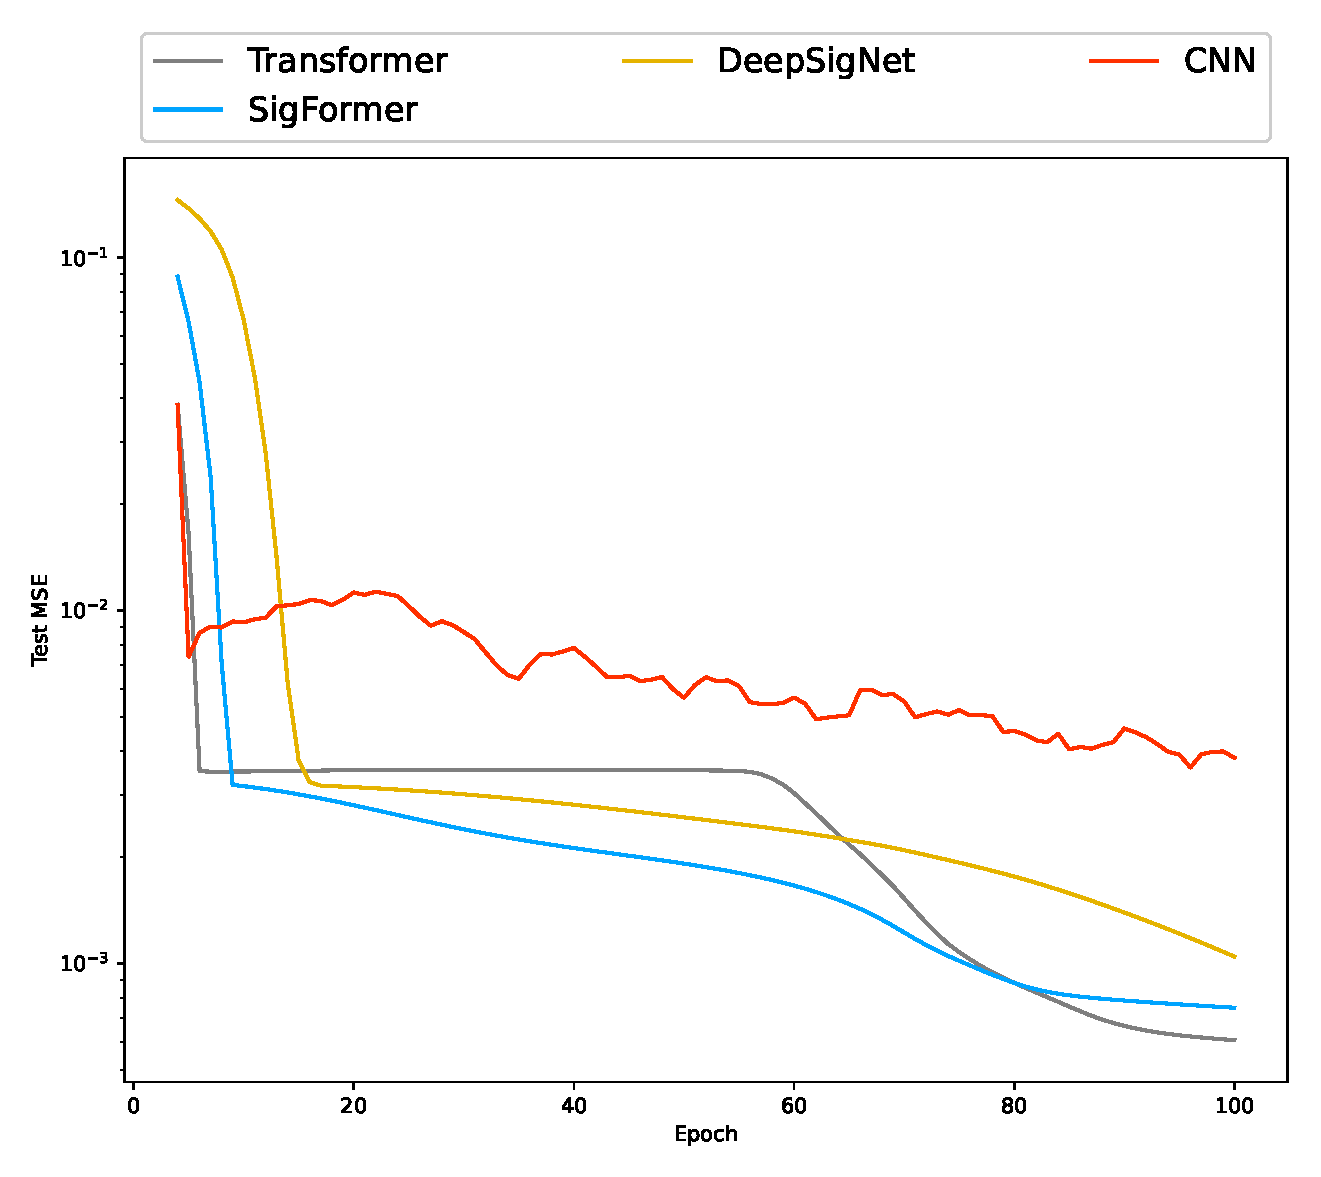
\includegraphics[width=0.32\textwidth]{fig//numerical_example4//loss_plots//input_length_500//rBergomi_grid=500_Hbeta_eta=1_v0=0.01.eps}
				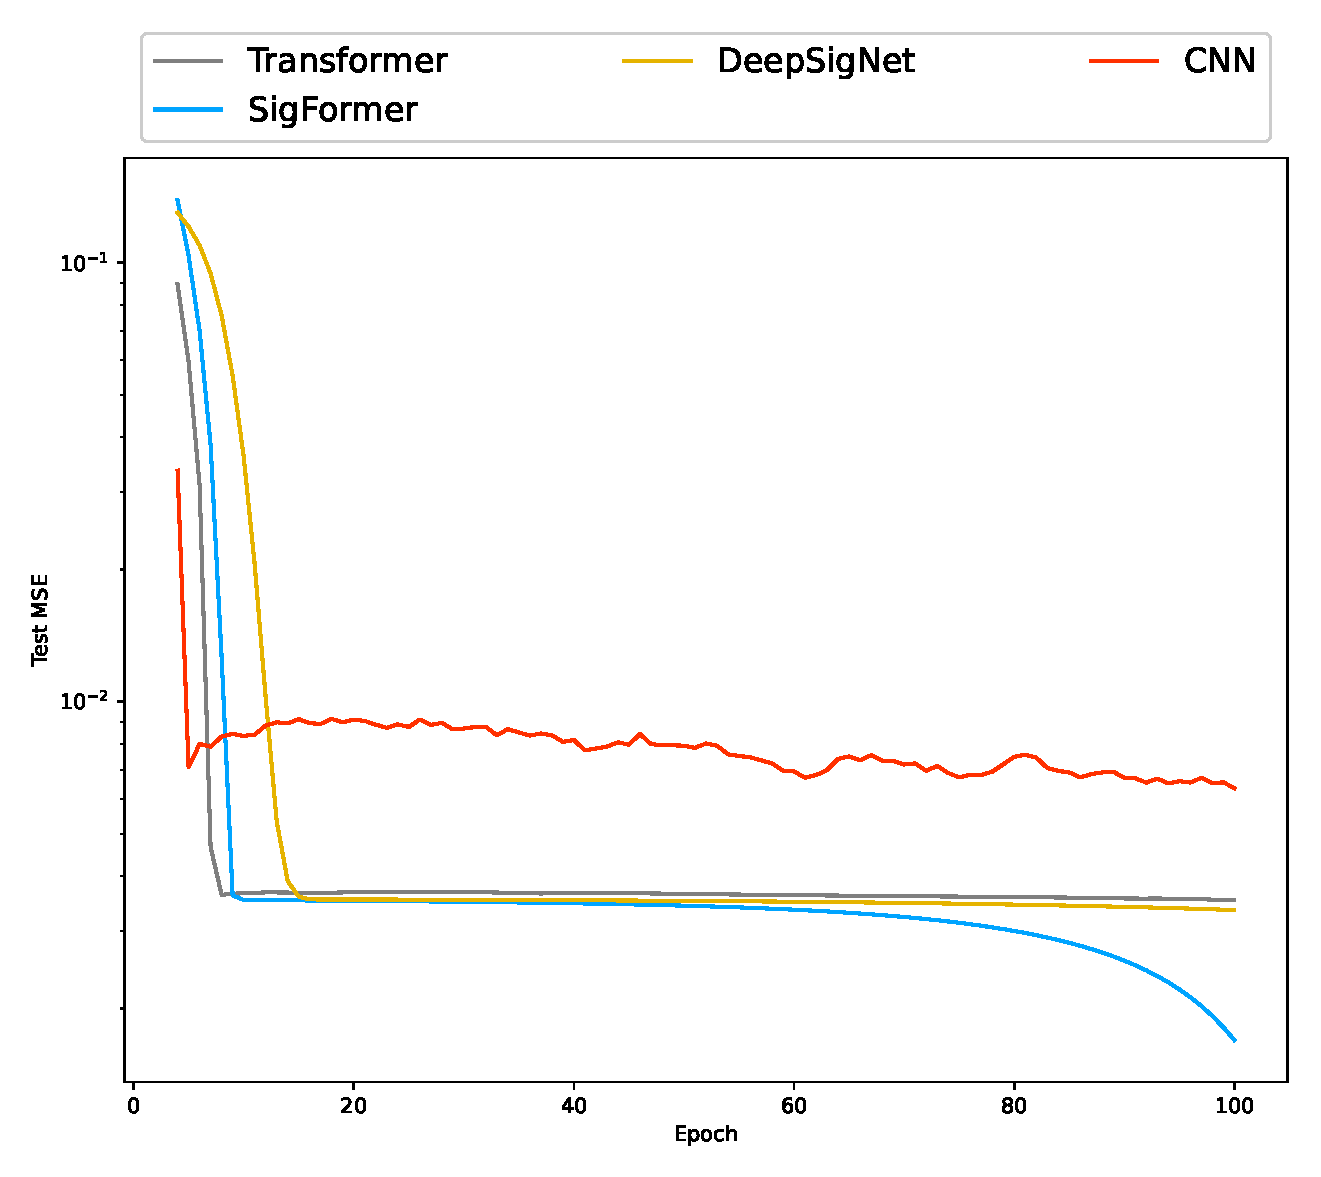
\includegraphics[width=0.32\textwidth]{fig//numerical_example4//loss_plots//input_length_500//rHeston_grid=500_Hbeta_kappa1=0.1_kappa2=0.03_theta=0.3_v0=0.01.eps}}
		}
		\caption{Loss plot for (Left:) fBms; (Middle:) rBergomi volatility processes; (Right:) rHeston volatility processes with input lengths equal to $500$. }
	\end{figure}
	
	\subsection{Loss plots for multiple parameters calibrations}
	\label{subapdix-loss-plots-calibration-multiple}
	\begin{figure}[H]
		\centering
		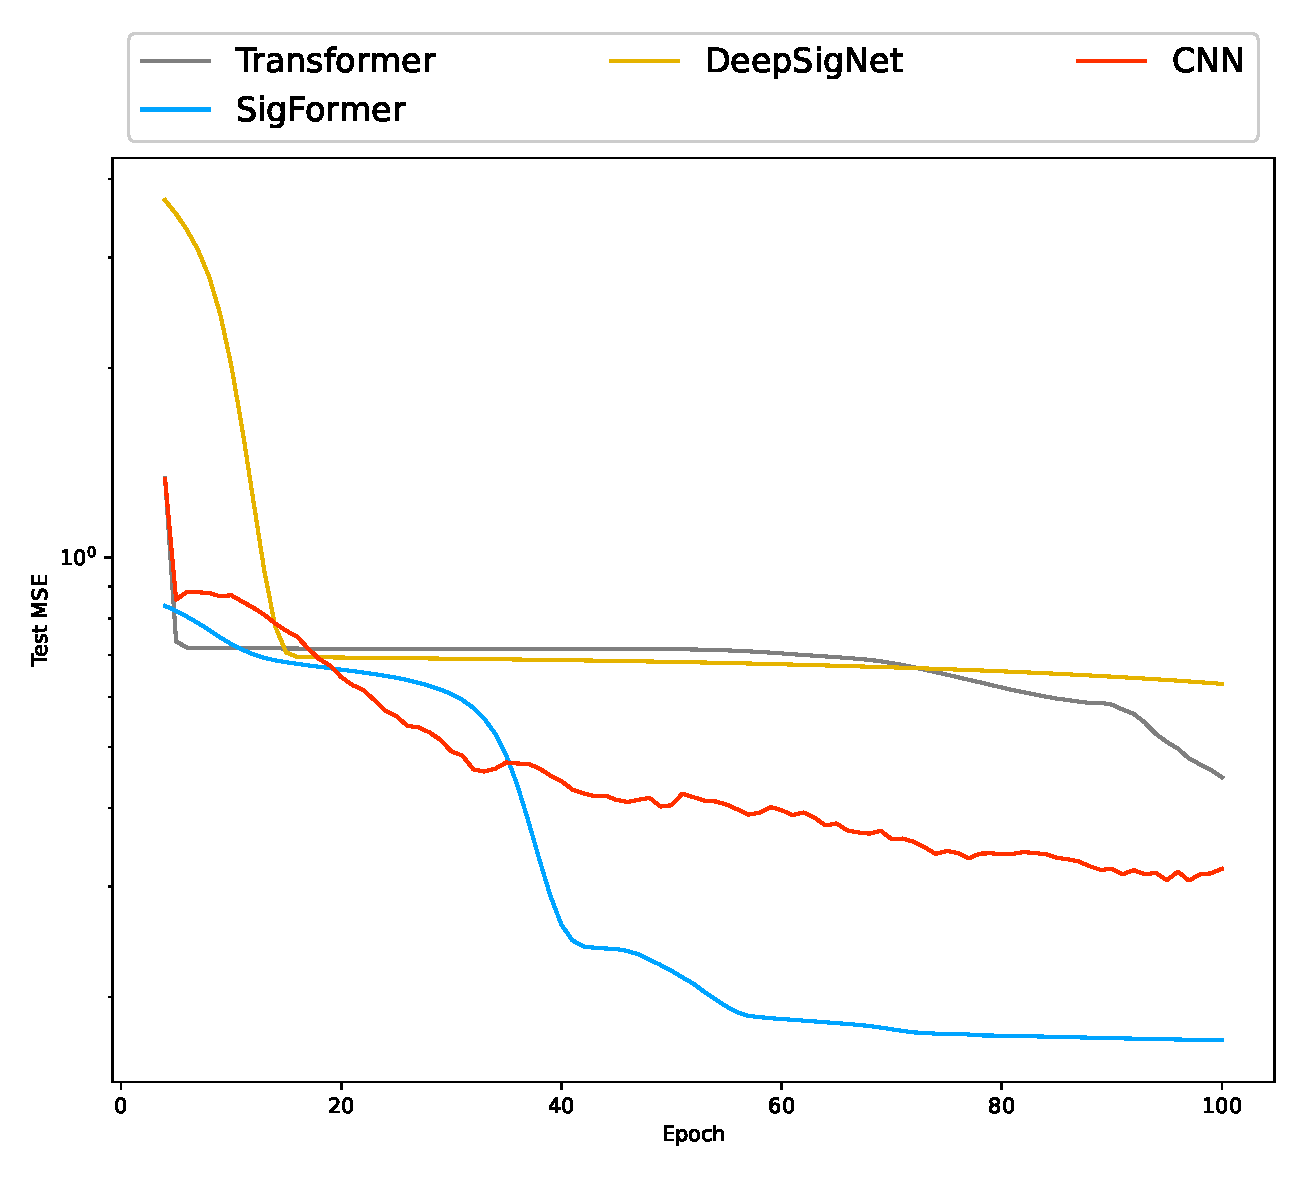
\includegraphics[width=0.45\textwidth]{fig//numerical_example5//loss_plots//rBergomi//rBergomi_grid=100_Hbeta_etauniform_v0=0.01.eps}
		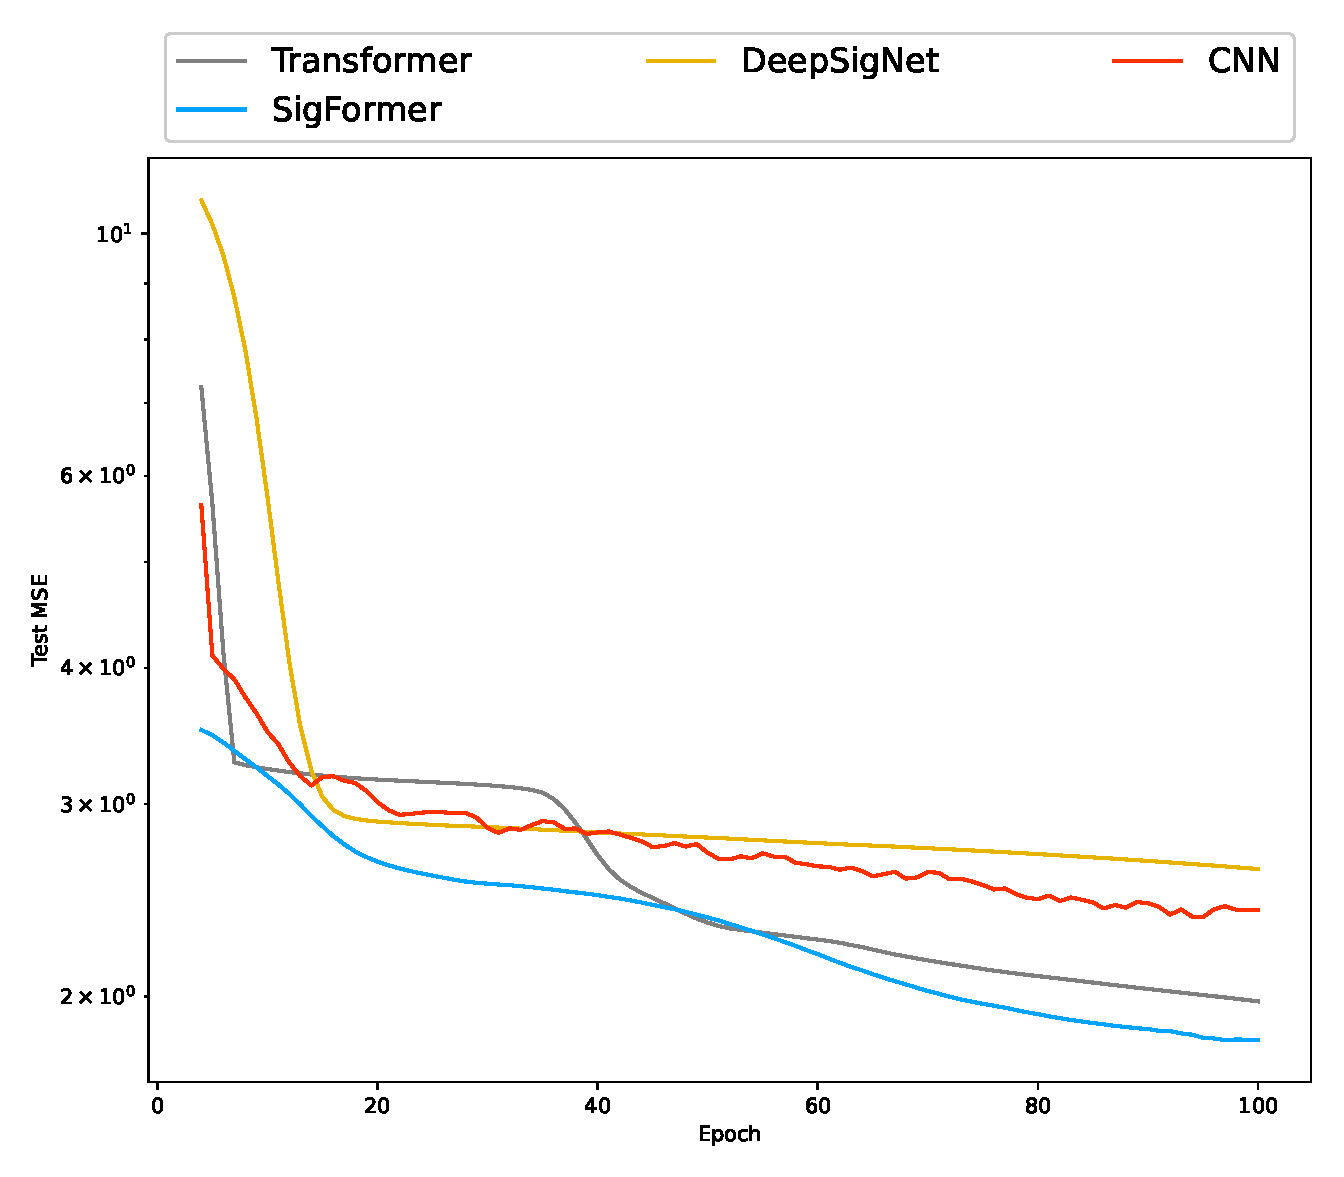
\includegraphics[width=0.45\textwidth]{fig//numerical_example5//loss_plots//rHeston//rHeston_grid=100_Hbeta_kappa1uniform_kappa2uniform_thetauniform_v0=0.01.eps}
		\caption{Loss plot of multiple parameters calibration for (Left:) rBergomi volatility processes and (Right:) rHeston volatility processes with $H\sim\text{Beta}(1,\,9)$, $\eta\sim\text{Uniform}(0,\,3)$, $\kappa_1\sim\text{Uniform}(0,\,5)$, $\kappa_2\sim\text{Uniform}(0,\,3)$ and $\theta\sim\text{Uniform}(0,0.5)$. }
	\end{figure}
	
	\subsection{Loss plots for empirical studies}
	\label{subapdix-loss-plots-empirical}
	\begin{figure}[H]
		\centering
		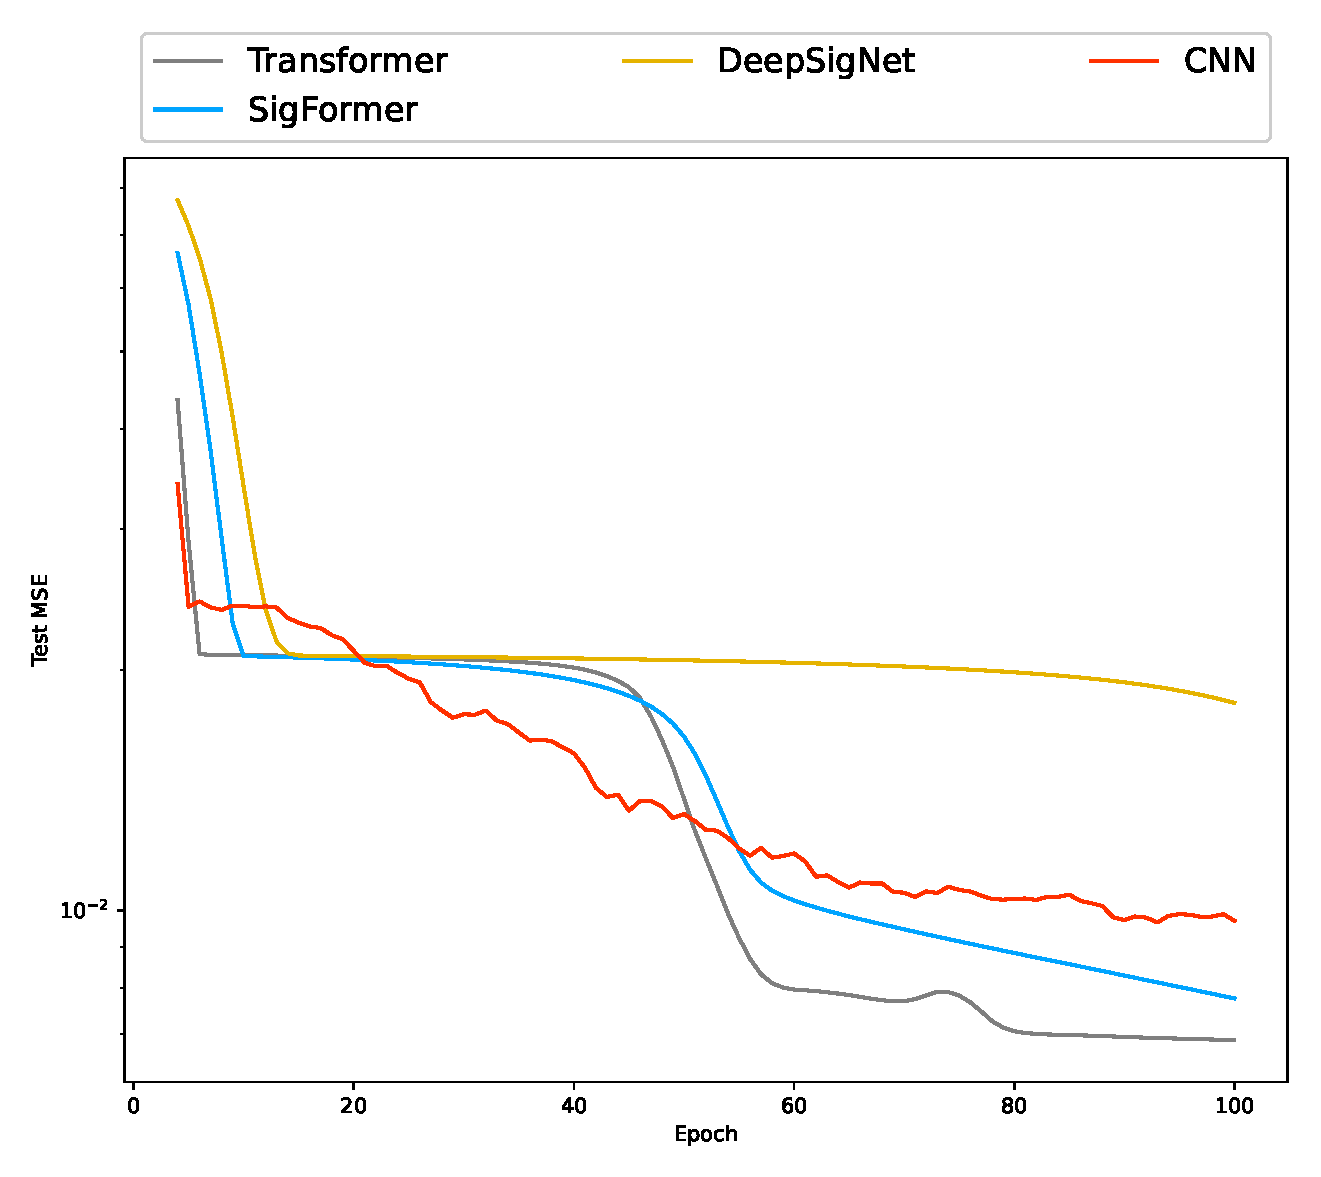
\includegraphics[width=0.45\textwidth]{fig//empirical_example6//loss_plots//rHeston_grid=100_Huniform_kappa1=0.1_kappa2=0.03_theta=0.3_v0=0.01.eps}
		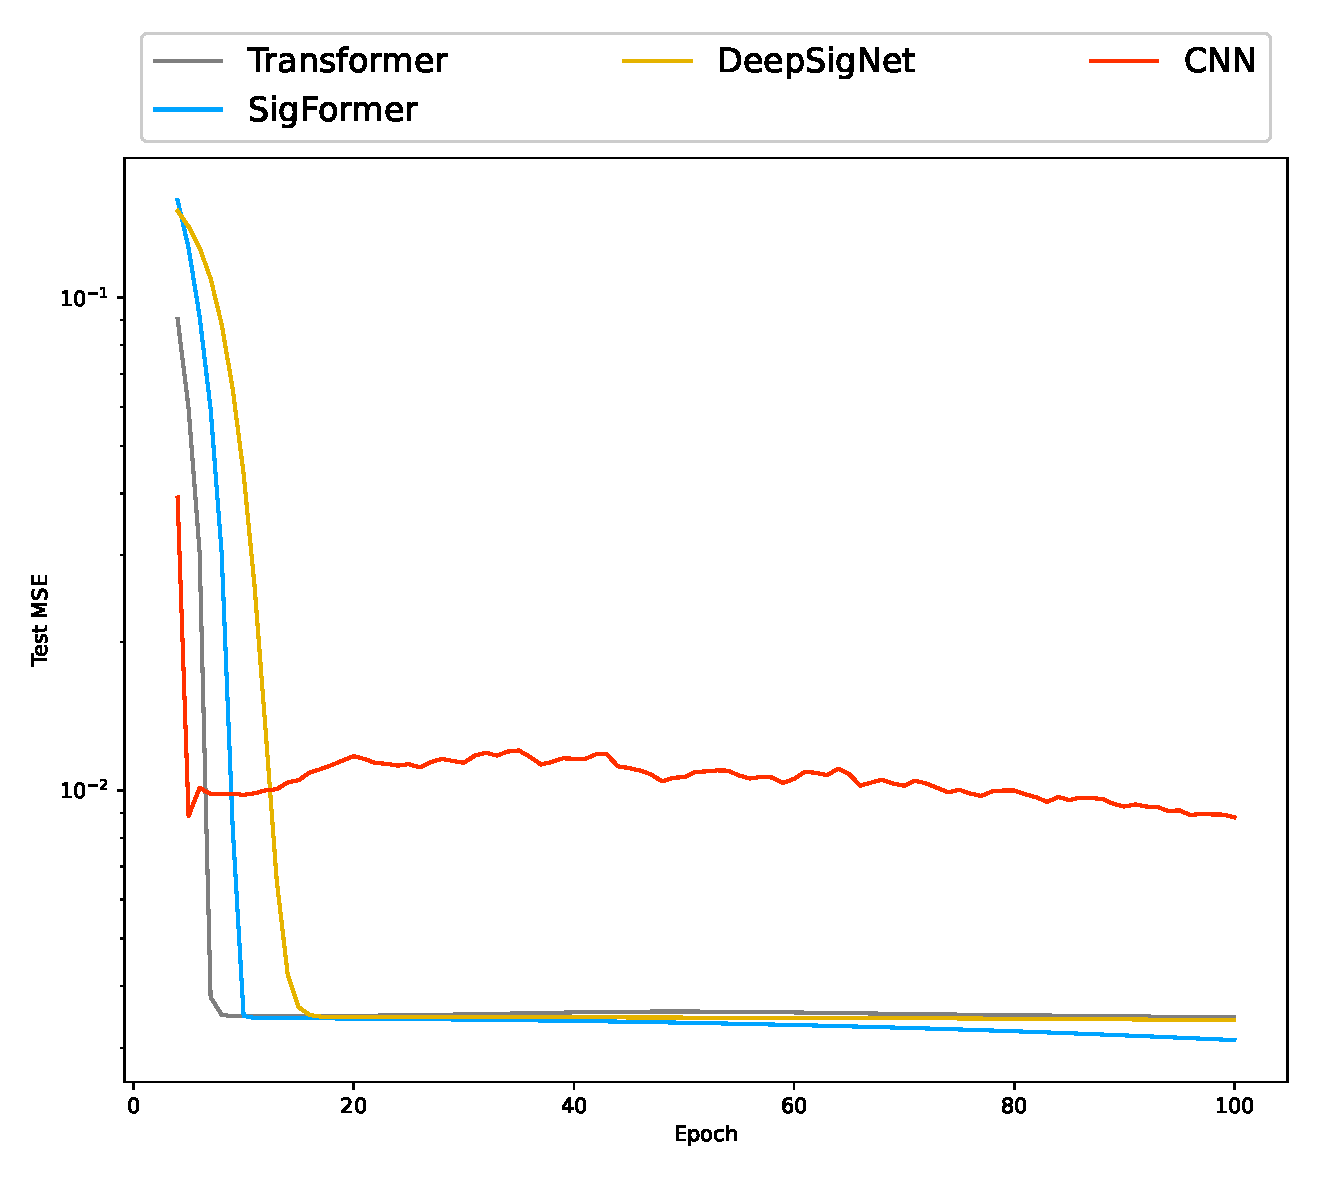
\includegraphics[width=0.45\textwidth]{fig//empirical_example6//loss_plots//rHeston_grid=100_Hbeta_kappa1=0.1_kappa2=0.03_theta=0.3_v0=0.01.eps}
		\caption{Loss plot of rHeston volatility processes with (Left:) $H\sim\text{Uniform}(0,0.5)$ and (Right:) $H\sim\text{Beta}(1,\,9)$. }
	\end{figure}
	

\end{document}
